    \documentclass[a4paper]{article}

\usepackage[utf8]{inputenc}
\usepackage[T1]{fontenc}
\usepackage[german,english]{babel}
\usepackage{graphicx}
\usepackage{lmodern}
\usepackage{amsmath}
\usepackage{amssymb}
\usepackage{wasysym}
\usepackage{xcolor}
\usepackage{hyperref}
\usepackage[toc,page]{appendix}
\usepackage{algpseudocode}
\usepackage{algorithm}
\usepackage{framed}

\definecolor{lighter-gray}{gray}{0.20}
\definecolor{light-gray}{gray}{0.30}
\hypersetup{pdfborder={0 0 0},colorlinks=true,urlcolor=lighter-gray,linkcolor=light-gray}

% definitions
\newcommand{\drawing}[1]{%
 \begin{figure}[ht]
  \begin{center}
   \includegraphics{#1}
  \end{center}
 \end{figure}
}
\newcommand{\pic}[2]{%
 \begin{figure}[ht]
  \begin{center}
   \includegraphics{#1}
   \caption{#2}
  \end{center}
 \end{figure}
}
\newcommand{\given}[1]{\textbf{Given.} #1\par}
\newcommand{\find}[1]{\textbf{Find.} #1\par}
\newcommand{\cls}[1]{\rm{#1}}
\newcommand{\probl}[1]{\text{\textsc{#1}}}
\newcommand{\card}[1]{|#1|}
\newcommand{\set}[1]{\left\{#1\right\}}
\newcommand{\dateref}[1]{\emph{This lecture took place on #1.}\par}
\newenvironment{spec}[0]{\begin{framed}}{\end{framed}}
\newenvironment{definition}[0]{\textbf{Definition.}}{}

\DeclareMathOperator{\detm}{det}
\DeclareMathOperator{\perm}{det}
\DeclareMathOperator{\sign}{sign}
\DeclareMathOperator{\prop}{probability}

% metadata
\title{
  Theoretical Computer Science 2 \\
  \large{University of Technology Graz} \\
  \normalsize{Lecture notes of a student}
}
\date{\today}
\author{Lukas Prokop}

% settings
\parindent0pt
%\setcounter{tocdepth}{2}
%\setlength{\parskip}{15pt plus 1pt minus 2pt}

\begin{document}
\maketitle
\tableofcontents
\newpage


\dateref{2nd of Oct 2013}
\subsection{Structure of this course}
%
Evaluation:
\begin{description}
  \item[Practicals] 2-3 board presentations
  \item[Lecture] oral exam (ask for date via email)
\end{description}

Contents:
\begin{itemize}
  \item Extended view on complexity theory and modern applications
  \item Focus on algorithms, optimization problems and cryptography
\end{itemize}

2 sections:
\begin{enumerate}
  \item Complexity theory
    \begin{itemize}
      \item randomized complexity classes
      \item polynomial hierarchy
      \item interactive protocols (zero knowledge systems)
      \item probabilistically checkable proof (PCP theorem)
    \end{itemize}
  \item Approximation of complexity
    \begin{itemize}
      \item complexity theory of heuristic algorithms
    \end{itemize}
\end{enumerate}

\subsection{Literature}
%
\begin{itemize}
  \item C. Papadimitriou, ``Computational complexity'', 1994 [old, classic].
  \item I. Wegener, \foreignlanguage{german}{,,Komplexitätstheorie (Grenzen in der Effizienz von Algorithmen)''}, 2003 [modern, non-comprehensive].
  \item S. Arora, B. Barak, Computational complexity (A modern approach), 2009 [modern, exhaustive].
\end{itemize}

\setlength{\parskip}{0.8\baselineskip}
\newpage


\section{Randomized complexity classes}
\subsection{Problem: Does a perfect matching exist in a given bipartite graph?}
\label{sec:perfect-matching-algorithm}
%
\subsubsection{Problem and approach}
%
\begin{spec}
  \given{$G = (U, V, E)$ is an undirected, bipartite graph with $U = \set{u_1, u_2, \ldots, u_n}$ and $V = \set{v_1, v_2, \ldots, v_n}$.}
  \find{Does a perfect matching exist in the bipartite graph $G$?}
  \textbf{Reference.} ``Computational Complexity'' (Christos Papadimitriou), ``Symbolic determinants'' in section 11.1
\end{spec}
\begin{definition}
  A \emph{matching} $M$ in $G$ is a set of pairwise non-adjacent edges. So no two edges of the matching share a common vertex. A \emph{perfect matching} is a matching covering all vertices of $G$.
\end{definition}

\textbf{Note.} This question can be answered in polynomial time with a deterministic algorithm (``Edmonds's algorithm'', $\mathcal{O}(\card{V}^4)$). We take a different approach.

\begin{figure}[h]
  \begin{center}
    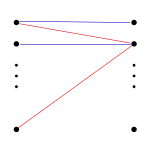
\includegraphics{tcs2_bipartite_graph_perfect_matching.pdf}
    \caption{Perfect matchings in a bipartite graph. Red edges show a perfect matching in the left graph. In the right graph no perfect matching exists.}
  \end{center}
\end{figure}

Consider a matrix $A(G) = (a_{i,j})$ for graph $G$. We distinguish 2 cases:
\[
  a_{i,j} = \left\{\begin{array}{cl}
    \underbrace{x_{i,j}}_{\text{symbolic variable}} & (u_i, v_j) \in E  \\
    0 & (u_i, v_j) \notin E
  \end{array}\right.
\]

$S_n$ is the set of permutations over $\set{1, \ldots, n}$.
\[
  \det A(G) = \sum_{\pi \in S_n} \sigma(\pi) \cdot \prod_{j=1}^n a_{j,\pi_j}
\] \[
  \sigma(\pi) = \begin{cases}
    1 & \pi \text{ is an even permutation} \\
    -1 & \pi \text{ is an odd permutation}
  \end{cases}
\]

Observation:
\begin{enumerate}
  \item Non-zero terms of the product in $\det A$ correspond to a perfect matching.
  \item $G$ has a perfect matching if the $\det A(G) \neq 0$ (hence is a zero function).
\end{enumerate}

Remarks:
\begin{itemize}
  \item This alternative method given above is based on the evaluation of $\det A(G)$.
  \item We are interested in the evaluation of a symbolic determinant.
\end{itemize}

For given values of $x_{i,j} \in \mathbb{Q}$ we can evaluate $\det A(G)$ in polynomial time (eg. via gaussian elimination).
For the symbolic determinant evaluation no algorithm is known (actually, the question whether a specific coefficient is the coefficient of the symbolic non-zero determinant, is an \cls{NP}-complete problem).

In our case we want to know whether or not $\det A(G) = 0$.

\subsubsection{Idea and Lemma}
%
Select a random configuration for $x_{i,j}$ and evaluate the resulting determinant.
If the determinant is 0, then we have found the zero function or a root in the function.
In the other case G has a perfect matching (result: YES).
In the first case, we have to proceed with further evaluations.

\textbf{Lemma 1.1:}
Assume $p(z_1, z_2, \ldots, z_m)$ to be a polynomial with $m$ variables (must not be the zero polynomial). $d$ is the maximum degree of those variables.
Furthermore $M > 0$ and $M \in \mathbb{Z}$. It is fact that the number of $m$-tuples $(z_1, \ldots, z_m) \in \set{0, 1, \ldots, M-1}$ with $p(z_1, \ldots, z_m) = 0$ is smaller or equal to $mdM^{m-1}$ (so this is the upper bound).

\textbf{Proof of the Lemma:} Complete induction over $m$.
\begin{description}
  \item[$m=1$:]
    Number of zeros $\leq d$ (with respect to the fundamental theorem of algebra)
    for a polynomial of 1 variable of degree $\leq d$.
  \item[$m-1 \rightarrow m$:]
    Polynomial $p$ in $z_1, \ldots, z_m$. Consider $p$ to be a polynomial in $z_m$ with coefficients
    which are in $z_1, \ldots, z_{m-1}$.
\end{description}

\textbf{Remark.}
  $p$ results in evaluation of ``gzz'' test tuple 0.

Case distinction:
\begin{description}
  \item[The coefficient with highest degree of $z_m$ in $p$ is 0.]
    Apply induction to the coefficient of $z_m$ with highest degree.
    The coefficient is a polynomial in $z_1, \ldots, z_{m-1}$.
    Can therefore $\leq (m-1)$ of $M^{m-2}$ permutations of $(z_1, \ldots, z_{m-1})$.
    In combination with the selection of $z_m$ ($M$ possibilities).
    $\leq (m-1)$ of $M^{m-1}$.
  \item[Is not $0$.]
    We have a polynomial of degree $\leq d$ in $z_m$ such that $\leq d$ null points
    can exist for each combination of $z_1, \ldots, z_{m-1}$.
    Therefore $\leq d$ $M^{m-1}$ further null points of $p$.
    Addition of $(m-1)$ in $M^{m-1}$ with $d$ with $M^{m-1}$ results in $\leq m\cdot d$ with $M^{m-1}$.
    So this lemma is proven.
\end{description}

Consider the following algorithm:
\begin{algorithm}
\caption{\href{http://www.cs.cmu.edu/afs/cs/academic/class/15859-f04/www/scribes/lec3.pdf}{Mulmuley, Vazirani and Vazirani (1987)}}
\begin{algorithmic}[1]
  \State
    Choose $m$ random integers ($i_1, \ldots, i_m$) for the assignment of $x_{i,j}$ with $\set{i,j} \in E$.
    (here $m = |E|$) with $x_{i,j} \in \set{0, \ldots, M-1}$ whereas in the case of a matching $M = 2m = 2\cdot |E|$.
  \State Evaluate $\det A(G)$ for $x_{i,j}$ assignment  ($i_1, \ldots, i_m$).
  \If{$\det A(G) (i_1, \ldots, i_m) \neq 0$}
    \State \Return ``Yes, G has a perfect matching''.
  \Else
   \State \Return ``I don't know'' (we need further repetitions).
  \EndIf
\end{algorithmic}
\end{algorithm}

This algorithm returns with ``no error'' or ``I don't know''.
This algorithm is part of the complexity class \cls{RP}.

\subsubsection{Analysis of the algorithm}
%
Properties of the algorithm (false-biased Monte-Carlo algorithm):
\begin{itemize}
  \item If the answer is Yes (there exists an perfect matching), the answer is always correct (no false positives).
  \item
    If the graph does not have a perfect matching, the answer of the algorithm is not complete.
    Consider the answer ``No'' if the number of repetitions with the answer ``I don't know'' exceeds
    some threshold (therefore, false negatives are possible).
\end{itemize}

\emph{What's the probability that we get a false negative?}

In the case of a Yes-answer we can see that the error probability (applying the algorithm once)
is $\leq \frac12$ (recognize that $d=1$ here).
With $k$ applications, we get a probability $\leq \frac{1}{2^k}$.

\subsection{Problem: SAT problem}
\label{sec:sat-algorithm}
%
\begin{spec}
  \given{A boolean equation $\phi$ in conjunctive normal form.}
  \find{Is $\phi$ satisfiable?}
  \textbf{2-SAT.} Restrict boolean equation to CNF with 2 literals per clause. \par
  \textbf{3-SAT.} Restrict boolean equation to CNF with 3 literals per clause. \par
\end{spec}

\probl{2-SAT} has been show to be polynomially decidable (eg. with flow theory).
Here the following algorithm shall be given:
\begin{algorithm}
  \caption{Algorithm to decide \probl{2-SAT} in polynomial time (Even, Itai, Shamir, 1976)}
\begin{algorithmic}[1]
  \State All variables are unassigned. Recent branch point is unknown.
  \While{unassigned variables exist}
    \If{both literals of clause falsify clause}
      \If{Backtracking not possible}
        \State \Return{Unsatisfiable}
      \Else
        \State Go back to most recent branch point.
      \EndIf
    \ElsIf{one of both variables of clause are set}
      \State Assign the remaining variable in a way to make clause satisfied
    \ElsIf{clause is satisfied or both variables are free}
      \State Create branch point
      \State Set one variable to an arbitrary value
    \EndIf
  \EndWhile
\end{algorithmic}
\end{algorithm}
%
%\emph{What is unit propagation?}
%\begin{itemize}
%  \item For every clause $(a \lor a)$, assign $a=\top$.
%  \item For every clause $(\neg a \lor \neg a)$, assign $a=\bot$.
%\end{itemize}

3-SAT is known to be \cls{NP}-complete and cannot be solved efficiently.

Consider the following algorithm for SAT:
\begin{algorithm}
\begin{algorithmic}[1]
  \State Start with a random assignment $T$ for the variables $x_1, \ldots, x_n$.
  \For{$r$ times}
    \If{$T$ is a satisfiable assignment}
      \State \Return yes.
    \EndIf
    \State Let $c$ be one of the clauses which are not satisfied.
    \State Take one literal of $T$ and negate its variable in the assignment.
  \EndFor
  \State \Return ``no'' or ``probably no''.
\end{algorithmic}
\end{algorithm}

Is also a Monte-Carlo-Algorithm.
Open issues: Probability for false negatives? How to choose $r$?

Is a polynomial upper bound of $r$ (in regards of the number of clauses) enough
for a practical error probability? (exponentially, it is easily feasible)

\begin{itemize}
  \item No, even for 3-SAT there are known instances of the problem where a polynomial $r$ fails.
  \item For 2-SAT for $r = 2n^2$ we have an error probability of $\leq \frac12$.
        Therefore we have a Monte-Carlo algorithm for 2-SAT.
\end{itemize}

\dateref{7th of Oct 2013}

\subsection{Problem: Polynomial Identity Testing}
\label{sec:identity-test-polynomials-algorithm}
%
\begin{spec}
  \given{A polynomial}
  \find{Is the given polynomial a zero-polynomial (hence equals to $0$)?}
  \textbf{Equivalence.} Be aware that \emph{polynomial identity testing} equals \emph{polynomial equivalence checking}. $p_1(x) = p_2(x) \Leftrightarrow [p_1(x) - p_2(x)] = 0$ \par
  \textbf{Example.} $- x\cdot x - y\cdot y + (x - y)(x + y)$ is a zero-polynomial whereas $x\cdot x$ is not. \par

  The instance can be encoded in various forms. Possible forms include:
  \begin{itemize}
    \item multivariate arithmetic expression over integers (arithmetic formula)
    \item matrix with polynomial entries
  \end{itemize}
\end{spec}

Polynomials are represented here as equations of an algebraic circuit (instead of the operators $\land, \lor$ and $\neg$ in classical propositional logic, we have $+$, $-$ and $\cdot$ available) with $n$ variables $x_1, x_2, \ldots, x_n$
represented as special directed graph. All vertices (which are not sources and are not inner vertices) do have in-degree 2 und are annotated with operators $\set{+, \cdot, -}$.

\begin{figure}[ht]
  \begin{center}
    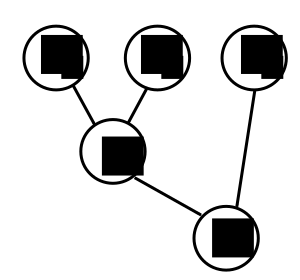
\includegraphics{tcs2_algebraic_circuit.pdf}
    \caption{Visual representation of algebraic circuit $x_1 x_2 + x_3$}
  \end{center}
\end{figure}

Remarks:
\begin{itemize}
  \item Extensions to this problem are possible.
  \item Such a circuit creates a polynomials in $x_1, x_2, \ldots, x_n$.
\end{itemize}

\subsubsection{The class \cls{ZeroP}}
%
Let \cls{ZeroP} be the complexity class of algebraic circuits,
which evaluate whether a polynomial (which is identical) is a zero-polynomial.

\[
    c = c' \quad \Leftrightarrow \quad c - c' = 0
\]
This is why the name \cls{ZeroP} was chosen. A special case of this problem is the previous problem to determine whether a perfect matching exists.

\textbf{Problem:} Detection of \cls{ZeroP} is non-trivial (ie. is a polynomial $P \in$ \cls{ZeroP}).

Consider for example
\[
  \prod_{i=1}^n (1 + x_i)
\]
This is a very compact description, but the circuit has size $2n = \mathcal{O}(n)$
but polynomial has $2^n$ terms.

For this problem no deterministic, efficient algorithms is known, but a
nice Monte-Carlo algorithm.

We can use the following Lemma 1.2 (analogous to Lemma 1.1):
\begin{quote}
  Is $p(x_1,\ldots,x_n)$ a polynomial of total degree $\max \tilde{d}$.
  For example $x_1^2 x_2^3 x_3 x_4^7$ has max-degree 13 for all terms.

  S is a finite set of integers. If $a_j,\ldots,a_n$ is selected randomly out of S.

  In this case:
  \[
    P(p(a_1, \ldots, a_n) \neq 0) \geq 1 - \frac{\tilde{d}}{\card{S}}
  \]
\end{quote}

A circuit $C$ of size $m$ contains $\leq m$ multiplications and therefore degree $\leq 2^m$.

Idea for probabilistic algorithm:
\begin{algorithm}
\caption{Probabilistic algorithm to solve ``is polynomial zero?''}
\begin{algorithmic}[1]
  \State
    Select random integers $I$ for $x_1, \ldots, x_n \in \set{1, \ldots, 10, \ldots, 2^m}$
    (requires $\mathcal{O}(nm)$ random bits).
  \State Let $Y$ be the result of the evaluation of $C$ for $I$.
  \State If $Y = 0$, answer ``Yes''. Else ``I don't know''.
\end{algorithmic}
\end{algorithm}

If $C \in \cls{ZEROP}$, then we accept $C$ always.
If $C \notin \cls{ZEROP}$ and we do not answer with ``NO'' for $y \neq 0$,
we have a error probability.
We reject $\leq \frac{1}{10} \cdot (\text{Mil probability} \geq \frac9{10})$.

\textbf{Problem:} Degree can be at maximum $2^m$. $y$ and the intermediate
results can grow up to $(10\cdot 2^m)^{2^m}$. An exponential number of bits
is necessary for representation. Therefore we would like to switch to modulo
calculations.

We evaluate $C \mod{k}$ where $k$ is randomly selected from $\set{1, \ldots, 2^{2m}}$
(further constraints are mentioned later).
Instead of $y$, we get $y\mod{k}$. If $y = 0$, then also $y \mod{k} = 0$.

If $y \neq 0$, then we can show that $k$ (with probability $\geq \delta = \frac1{4m}$)
does not split. This probability is small enough that $\mathcal{O}(\frac1{\delta})$
are enough repetitions to gain our result.
We do only accept $a^k$, if for all runs the result was $0$.

Is $y \neq 0$ and $B = \set{p_1, \ldots, p_n}$ the set of distinct prime factors
of $y$. This satisfies that $K$ is not a prime number of $B$ is given with probability $\geq \delta$.
With the prime number theorem, we can conclude that for sufficient large $m$
the number of prime numbers in $\set{1, \ldots, 2^{2m}}$ is $\geq \frac{2^{2m}}{2\cdot m}$.

$y$ can have $\max \log{y} \leq 5, m\cdot 2^m = o(\frac{2^{2m}}{2m})$ prime factors.

For sufficiently large $m$ it is given that the number of $k \in \set{1,\ldots,2^{2m}}$
such that $k$ is prime and $k \notin B$: $\geq \frac{2^{2m}}{4m}$
with probability $\delta = \frac{1}{4m}$ a random $k$ has the desired properties.

\subsection{Problem: Primality testing}
\label{sec:primality-test-algorithm}
%
In the meantime a deterministic polynomial primality test is known
(Agrawal, Kayal, Saxena). For a few years only randomized primality tests
(which represent Monte Carlo algorithms) were known.

\begin{spec}
  \given{$n$ is odd}
  \find{Is $n$ not a prime number?}
\end{spec}

\subsection{Probabilistic complexity classes overview}
%
In this section we want to given a quick overview for the definitions required to discuss this topic.
See table~\ref{tab:prob_compl_classes} for the class overview.

\begin{table}
 \begin{center}
  \begin{tabular}{ccc}
   \hline \hline
      & failure/error probability & failure/error probability \\
      & (bounded) & (not bounded) \\
   \hline
     Two-sided error & \cls{BPP} & \cls{PP} \\
   \hline
     One-sided error & \cls{RP}, \cls{co-\cls{RP}} & \cls{NP}, \cls{co-NP} \\
                     & \cls{RP} = Monte-Carlo algorithms & \\
   \hline
     No error, & $\cls{ZPP} = \cls{RP} \cap \cls{co-\cls{RP}}$ & $\cls{NP} \cap \cls{co-NP}$ \\
     but failure is possible & (Las Vegas Algorithms) & \\
   \hline
     No error, no failure & \cls{P} & \\
   \hline \hline
  \end{tabular}
  \caption{Probabilistic complexity classes overview}
  \label{tab:prob_compl_classes}
 \end{center}
\end{table}

Now we would like to formalize Monte-Carlo algorithms.
Monte-Carlo turing machines are special cases of probabilistic turing machines.
Probabilistic turing machines are a generalization.

\subsection{Monte-Carlo turing machines and \cls{RP}}
%
\textbf{Definition.} $N$ is a polynomial, non-deterministic turingmachine.
We assume for $N$ that all computations for an input $x$ take the same number
of steps. This number has to be polynomial in $\card{x}$, because $N$ is
a polynomial turingmachine. Furthermore in every step there are exactly 2 non-deterministic decision possibilities.

$L$ is a language. $N$ is called Monte-Carlo turing machine for $L$ iff
$N$ satisfies the definition above and the computations for an input
of size $N$ are finished in $p(n)$ runtime (with $p$ as a polynomial) .
Furthermore it satisfies:
\begin{itemize}
  \item
    If $x \notin L$ then all computations of $N$ for $x$ end with the result ``No'' (no false positives).
  \item
    If $x \in L$ then more than half of the evaluations for x result in ``Yes''. Hence the probability of false negatives is $\leq \frac12$ where $\frac12$ is a configurable constant.
\end{itemize}

\cls{RP} (randomized polynomial) is a historical name and does not really distinguish
it from other classes.

The set of all languages for which there exists a Monte-Carlo turing machine
is called \cls{RP}.

\textbf{Remark:}
\begin{itemize}
  \item This concept corresponds to the informal concept of Monte-Carlo algorithms (of our exercises).
  \item If we replace the allowed error probability for false negatives to a value $\neq \frac12$, but $< 1$, no new complexity class is created.
\end{itemize}

Repetitions:
\[
    1-\epsilon \text{ with } \epsilon < \frac12 \text{ is the error probability of false positives}
\]
For k repetitions: Error probability for false negatives is $(1 - \epsilon)^k$. Choose k:
\[
    k = \left\lceil - \frac{1}{\log_2(1-\epsilon)} \right\rceil
        \text{  probability for false negatives is } \leq \frac12
\]

Runtime $k\cdot p(n)$ is polynomial for polynomial $k$.

\cls{RP} lies between \cls{P} and \cls{NP}. \cls{co-\cls{RP}} is the complement of \cls{RP} (ie. the result ``Yes''/``No''/``I don't know'' is exchanged).

\subsection{Complexity class \cls{ZPP}}
\label{class:ZPP}
\label{class:rp}
\label{class:co-rp}

\cls{ZPP} (polynomial randomized with zero probability of error)

\centerline{\cls{ZPP} = \cls{RP} $\cap$ \cls{co-\cls{RP}}}

In other words, there exists a Monte-Carlo algorithm which does not return
any false positives and an analogon which does not return false negatives
(no error, but failure is possible). This is the definition of Las-Vegas algorithms.

If probability of false positives and false negatives $\leq \frac12$ (after $k$ repetitions).

\subsection{Complexity class \cls{PP}}
\label{class:pp}

\cls{PP} (probabilistic polynomial) is not defined algorithmically. We consider \probl{MajSat} (majority SAT).

\begin{spec}
  \given{A SAT equation with $n$ variables.}
  \find{Determine whether the majority of $2^n \geq 2^{n-1}+1$ assignments satisfy the equation?}
\end{spec}

It is unknown whether or not \probl{MajSat} $\in$ \cls{NP} (how should the polynomial certificate look like?). It is even more unlikely that \probl{MajSat} $\in$ \cls{RP}.

\textbf{Definition.} (\cls{PP}) A language $L$ is in \cls{PP}, iff there is a non-deterministic polynomial TM $N$ (N satisfies the basic constraints mentioned above) such that for all inputs $x$ it states that
\[
    x \in L \quad \Leftrightarrow \quad \text{\#(computations of N for x result in ``YES'')} > \frac12
\]
Therefore this turing machine has an inherent majority evaluation capability.

\textbf{Remark:} Definition of \cls{PP} is syntactically, but not semantically.
We can easily show \probl{MajSat} $\in$ \cls{PP} and \probl{MajSat} is \cls{PP}-complete.

\dateref{9. Okt 2013}
%
\subsubsection{$\cls{NP} \subseteq \cls{PP}$}
%
\textbf{Proof.}
$L \in \cls{NP}$. $N$ is a non-deterministic turing machine for $L$.
We construct another turing machine $N'$, which decides $L$ with a majority vote.
$N'$ almost looks alike $N$. We introduce a new Start state and another
branching (non-deterministic decision), which is executed in the Start state.

Start state - non-deterministic choice which branch to take:
\begin{enumerate}
  \item Evaluation with $N$
  \item Randomized selection of one evaluation path
         (for all inputs $x$ of same size answer always with ``YES'').
\end{enumerate}

Consider input $x$. $x$ takes $p(\card{x})$ steps in $N$ (fundamental assumption as always).
\[
    2^{\card{x}}  \text{  evaluation paths of N for x}
\] \[
    2^{\card{x} + 1}  \text{  evaluation paths of N' for x}
\]

A majority of evaluations for $N$' for $x$ ends with ``Yes''.
This corresponds to: more than 1 evaluation of $N$ for $x$ ends with ``YES''.
This corresponds to $x \in L$.

We can conclude $L \in \cls{PP}$.

Remarks:
\begin{itemize}
  \item \cls{PP} is closed under complement.
  \item \cls{PP} is (in difference to our previous mentioned complexity classes)
         not algorithmically defined.
\end{itemize}

\subsection{The class \cls{BPP}}
\label{class:bpp}
%
\textbf{Definition.} \cls{BPP} (bounded error probabilistic polynomial)
contains all languages $L$ for which there is a non-deterministic
polynomial turing machine $N$ (without further constraints of the
assumptions with our fundamental assumptions) such that:

\begin{itemize}
  \item For all inputs $x$ with $x \in L$ ends with probability $\geq \frac34$
         of the evaluations of $N$ of $x$ with acceptance.
  \item For all inputs $x$ with $x \notin L$ ends with probability $\geq \frac34$
         of the evaluations of $N$ of $x$ with rejection.
\end{itemize}

Remarks:
\begin{itemize}
  \item Any value $> \frac12$ and $<1$ can be used instead of $\frac34$.
  \item For $\frac34$: $\frac14$ error probability for false positives 
         and false negatives.
  \item \cls{RP} $\subseteq$ \cls{BPP} (Monte-Carlo algorithm with error probability
         $\frac12$ repeated twice in different direction)
  \item \cls{co-\cls{RP}} $\subseteq$ \cls{BPP}
  \item \cls{BPP} $\subseteq$ PP (can easily be derived from the definition;
         has fewer constraints)
  \item Open issues:
    \begin{itemize}
      \item \cls{BPP} $\subseteq$ \cls{NP}?
      \item $\exists$ \cls{BPP}-complete problems?
    \end{itemize}
  \item \cls{BPP} is closed under complement.
  \item \cls{BPP} is basically a model for ``\emph{practical} polynomial randomized algorithm''.
\end{itemize}

All these complexity classes require some concept of probability;
for example random bits set on the turing machine. Question in practice:

Assume we don't have any fair dice / coins ($\prop{(\text{heads})} \neq \frac12$).
Does this define a new complexity class?

You can create a fair die with polynomial effort using an unfair die.
So \cls{RP} and \cls{BPP} (etc) are not influenced.

Take a coin with $\prop{(\text{heads})} = \rho$ with $\rho \neq \frac12$.
The following two lemmas apply:
\begin{enumerate}
  \item (Lemma 1.3) A coin with $\prop{(\text{heads})} = \rho$ can be simulated
         by a probabilistic, polynomial turing machine in expected time
         $\mathcal{O}(1)$, if the i-th bit of $\rho$ is determinable
         in polynomial time in $i$.
         Notice that the last assumption is only relevant for irrational
         numbers.
  \item (Lemma 1.4) A coin with $\prop{(\text{heads})} = \frac12$ (fair coin)
        can be simulated with a coin of $\prop(heads) = \rho$ in expected time
        $\mathcal{O}\left(\frac{1}{\rho (1-\rho)}\right)$.
\end{enumerate}

\subsubsection{Proof of Lemma 1.3}
%
Is $0.p_1 p_2 p_3\ldots$ a binary fractional representation of $\rho$.
The probabilistic turingmachine creates a sequence of random bits
$b_1 b_2 \ldots$ step by step, where bit $b_i$ is created in step $i$.
If $b_i < p_i$ then the turing machine returns ``heads'' as result and stops.
If $b_i > p_i$ then the turing machine returns ``tails'' as result and stops.
In any other case, go on (increment $i$).

If turing machine reaches bit $i+i$, then
\[
    b_j = p_j  \quad \forall j \in \set{1,\ldots,i}
\]
The probability for this is defined by $(\frac12)^l$.

The probability that the result is heads is $\sum_i p_i \cdot \frac{1}{2^i} = \rho$.
Expected runtime is $\sum_i i^c \cdot \frac{1}{2^i}$ for constant $c$.

\subsubsection{Proof of Lemma 1.4}
%
We construct a turing machine which simulates (using the possibility to
use a coin with $\prop(heads) = \rho$ multiple times) a fair coin.

M throws pair of coins (2 coins) with bias $\rho$. Repeat these paired throws
until 2 different results are given. We return ``heads'' for the result
heads-tails and ``tails'' for tails-heads.

Probability for heads-tails is $\rho \cdot (1-\rho)$.
Probability for tails-heads is $(1-\rho) \cdot \rho = \rho \cdot (1 - \rho)$.
Probability that turing machine stops in every step is $2\rho \cdot (1-\rho)$.
The conditional probability for stopping in step $k$ is equal for heads
and tails. So we can create a fair coin with $\prop(heads) = \frac12$.
This proof does work for any value of $\rho$.

\subsubsection{Remark for Lemma 1.2}
%
The ``probabilistic turing machine'' must have two transition function
$\delta_0$ ad $\delta_1$. We decide in every step whether we want to use
(with probability $\frac12$) $\delta_0$ or (with probability $\frac12$)
$\delta_1$. In the general model for a probabilistic turing machine
which is considered for efficient algorithms we allow expected polynomial
time.

From this lemma it follows that (if we allow expected polynomial
time\footnote{which is realistic for practical applications})
we don't lose any properties for a biased coin.
We can also show this for polynomial runtime rather than expected runtime
(by splitting the bitstring into blocks).

\subsection{Relations of probabilistic complexity classes}
%
\begin{figure}[ht]
  \begin{center}
    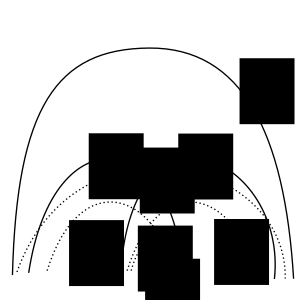
\includegraphics{randomized_complexity_classes.pdf}
    \caption{Overview of randomized complexity classes}
    \label{fig:complexity-classes}
  \end{center}
\end{figure}

Figure~\ref{fig:complexity-classes} gives an overview of randomized complexity classes.

The position of \cls{BPP} is partially unknown; partially we will discuss them later on.

The aspect of expected polynomial runtime is considered at a different place.

\section{The class \cls{FP}}
\label{class:fp}
%
\textbf{Definition.} (Complexity class of function problems for polynomial hierarchy).
Many problems in practice are no decision problems (they result in complexer
answers than ``YES'' or ``NO''). Two examples are FSAT and TSP.

\subsection{Problem: FSAT}
\label{sec:fsat}
%
\begin{spec}
  \given{A SAT equation $\phi$.}
  \find{Is there any satisfying assignment for $\phi$? If so, return it. Otherwise report ``No''.}
\end{spec}

Assume that a polynomial SAT algorithm exists for the decision problem SAT,
then we can solve FSAT in polynomial time:
$\phi$ is a SAT equation with variables $x_1, x_2, \ldots, x_n$.
\begin{enumerate}
  \item Apply SAT algorithm to $\phi$. If answer is ``no'', then
         $\phi$ is not satisifiable and we return ``there is no satisfying
         assignment''.
  \item (Successive fixation of variables.)
         We know that in one of the cases (true/false) the answer is ``Yes''
         and an assignment can be found. Fix variable $v$ in such a way
         (i.e. $\phi_1$ or $\phi_2$) that $\phi$ satys satisfiable.
         Stop if all variables got fixated.
         \drawing{fsat.pdf}
\end{enumerate}

This approach takes $\mathcal{O}(n)$ SAT calls.

\subsection{Problem: Travelling Salesman Problem (TSP)}
\label{sec:tsp}
%
\[
    D = (d_{ij}) \qquad d_{ij} \in \mathbb{Z}_0^+
\]
where $d_{ij}$ specifies the distance between the vertices $i$ and $j$.
$D$ is called distance matrix.

\begin{spec}
  Classical definition of TSP \par
  \given{Distance matrix $D$}
  \find{A hamiltonian path with minimum length/weight}
\end{spec}

Specifically, TSP is given as decision problem $\text{TSP}_{\text{DEC}}$:
\begin{spec}
  \given{$n \times n$ matrix $D = (d_{ij})$ with $d_{ij} \in \mathcal{Z}_0^+$ with upper bound $d^*$ of costs}
  \find{Is there any hamiltonian path of length $\leq d^*$?}
\end{spec}

\dateref{14th of Oct 2013}

We show that when a polynomial algorithm for $\text{TSP}_{\text{DEC}}$ exists, then there is a polynomial algorithm for TSP:

\paragraph{Step 1}
Determine the requested target function value (length of optimal tour).

Value of an optimal tour is in $\set{0,1,\ldots,2^q}$ with $q$ as the coding length
of the instance.

Binary search for the optimal value for the optimal value. Always ask:
is there any tour with length ($\leq 2^{q-1}$)? We get a binary tree always
with two branches ``Yes'' and ``No''. On the second level we ask is there any
tour with length ($\leq 2^{q-2}$).

After a polynomial number $\mathcal{O}(\log_2(2^q) = \mathcal{O}(q)$ of steps,
$c^*$---the length of the requested tour---is known.

\paragraph{Step 2}
Determine a required tour (a tour with length $c^*$).
Consider the values of $D$ in arbitrary order one after another.
$d_{ij}$ is the current item we look at. Then set $d_{ij}$ temporarily to $c^* + 1$
(Idea: restrict usage of $(i,j)$) and ask whether there is a tour of length $\leq c^*$
for the current matrix.

If answer is no, then we have to use the current edge $(i,j)$ and we set $d_{ij}$ back
to its old value. In the other case we keep $d_{ij}$ as $c^* + 1$.

In the end (after $\mathcal{O}(n^2)$ steps) we know the optimal tour.

\paragraph{Formally}
$L$ is a language in \cls{NP}. We want to define the associated function problem to L: FL.
For $L \in $ \cls{NP} there is a binary relation $R_L$, which is determinable in polynomial
time such that $\forall x \text{ strings } \exists \text{ string } y$ with
$\underbrace{R_L(x,y)}_{(x,y) \in R_L} \Leftrightarrow x \in L$. $R_L(x,y)$ is the
certificate of an accepted instance. 

\textbf{Definition.} (FL) Is $L \in \cls{NP}$ the associated problem FL for L.
Given a string $x$ we have to find a string $y$ such that $R_L(x,y)$ or answer that
there is no such $y$.

\paragraph{Next task:} Generalize the class / reduction term of decision problems for function problems.

\textbf{Definition:} A and B are two function problems. A is \emph{reducible to B}, iff $\exists$ string functions $R$ and $S$ (both computable in polynomial space) such that the relation illustrated in Figure~\ref{fig:function-problem-reduction} is given.

\begin{figure}[ht]
  \begin{center}
    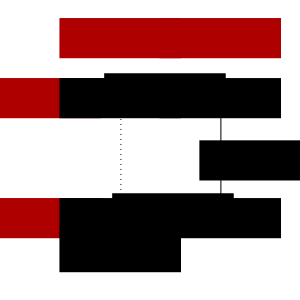
\includegraphics{function_problem_reduction.pdf}
    \caption{Reduction term for function problems}
    \label{fig:function-problem-reduction}
  \end{center}
\end{figure}

$x$ is an input string of an instance of $A$ such that $R(x)$ is an input string of an instance
of $B$. Is $z$ a correct output for the instance of $B$ with input $R(x)$ then $S(z)$ is a
correct output for the instance with input $x$.

\textbf{Remark:} Any logarithmic boundary for space implies polynomial time.

\textbf{Definition.} A function problem $A$ is says to be \emph{complete for a class
FC} of function problems iff $A \in$ FC and all problems in FC can be reduced to $A$.

We can show that FSAT $\in$ F\cls{NP} is F\cls{NP}-complete.

We want to consider a special class of function problems. They are problems for which there
are always valid solution and as such the answer is never ``No''. Example for such a problem:
$\exists$ always $y$ with $R_L(x,y)$?

\subsection{Problem: Factorization of integers}
\label{sec:integer-factorization}
%
\begin{spec}
  \given{A number $n \in \mathbb{N}$}
  \find{prime number decomposition}
\end{spec}

The corresponding decision problem is not interesting (answer is always yes).
Function problems are not trivial. It's an open question whether factorization is possible
in polynomial time.
Factorization is fundamentally different than FSAT where a decision problem cannot be solved
efficiently.

\textbf{Definition.} (total functions) For such function problems there is always a valid solution.

\textbf{Definition.} We consider a problem $L$ in F\cls{NP} total, when for all strings $x \exists$
string $y$ $\exists$ with $R_L(x,y)$.

\textbf{Definition.} (TF\cls{NP}) partial class of all function problems with total functions.

\subsection{Exercise 2: Integer sets of same sum}
\label{sec:same-sum-integer-sets}
%
\begin{spec}
  \given{$n$ numbers $a_1, \ldots, a_n \in \mathbb{Z}^+$ with $\sum_{i=1}^n a_i < 2^n-1$.}
  \find{$I, J \subset \set{1,\ldots,n}$ with $I \neq J$ such that $I \cap J = \diameter$ (not always required) and $\sum_{i\in I} a_i = \sum_{i\in J} a_i$ (or answer ``No'' if there are no such sets).}
\end{spec}

For the special case $\sum_{i=1}^n a_i < 2^n -1$ there is always a solution due to the
pidgeonhole principle. Without this constraint, the decision problem is complete.

\subsection{Exercise 3: Happy net problem}
\label{sec:happy-net-problem}
%
\begin{spec}
  \given{Undirected graph $G$, edge weights $w_e \in \mathbb{Z}$ for all $e \in E$. State function $S$: $V \rightarrow \set{+1, -1}$.}
  \find{Find a state $S$ in which all vertices are happy.}
\end{spec}

A vertex $i \in V$ is called ``happy for $S$'' iff
\[ S(i) \cdot \sum_{\set{i,j}\in E} S(j) \cdot w_{ij} \geq 0 \]

\drawing{happy_vertices.pdf}

\textbf{Claim.} There always is such a state. \\
\textbf{Proof.} Potential function $\rho[s] := \sum_{\set{i,j} \in E} S(i) \cdot S(j) \cdot w_{ij}$.

\textbf{Remark.} $i$ is unhappy for $S$.
\[
    \underbrace{S(i) \cdot \sum_{\set{i,j} \in E} S(j) \underbrace{w_{ij}}_{\in \mathbb{Z}} < 0}_%
        {=-\delta \text{ with } \delta > 0, \delta \in \mathbb{Z} \text{ and therefore } \delta \geq 1}
\]

Transition $S \rightarrow S'$ with $S'(j) = S(j) \forall j \neq i$ and $S'(i) = -S(i)$ (flip) otherwise.
We can show that:
\[
    \rho[S'] = \rho[S] + 2\delta
\]

We come up with an algorithm from this:
\begin{quote}
  Start with a random start state. As long as there are unhappy vertices, flip them.
  Because there are $\rho$ values in $[-W, W]$ with $W = \sum_{\set{i,j} \in E} \card{w_{ij}}$
  and $\rho$ increases with $\geq 2^{\set{i,j} \in E}$, we have shown the finiteness
  of the algorithm.
\end{quote}

This is also a total function problem. The algorithm has pseudo-polynomial runtime (because
it depends on pseudo-polynomial property of $W$). It is an open question whether there exists
a polynomial algorithm.

\begin{spec}
  \given{An undirected graph ($G = (V, E)$) and a hamiltonian cycle $Q$ in G.}
  \find{A second hamiltonian cycle (but does not have to exist) (different from $Q$).}
\end{spec}

For cubic graphs (3-regular\footnote{$d(v) = 3 \forall v \in V$})
there is always a second hamiltonian cycle (if there is at least one).

Is a total function problem and it is open whether there is a polynomial algorithm.

\drawing{fnp.pdf}

\subsection{Four variants of TSP}

\subsubsection{TSP$_{\text{DEC}}$}
%
\begin{spec}
  \given{$n\times n$ matrix D and a boundary $c^*$.}
  \find{Is there a tour with length $\leq c^*$?}
\end{spec}

\subsubsection{\probl{Exact-TSP}}
%
\begin{spec}
  \given{$n\times n$ matrix $D$, value $c^*$}
  \find{Does the optimal tour has length $c^*$?}
\end{spec}

\subsubsection{\probl{TSP-Cost}}
%
\begin{spec}
  \given{$n\times n$ matrix $D$.}
  \find{Length of the optimal tour}
\end{spec}

\subsubsection{TSP}
%
\begin{spec}
  \given{$n\times n$ matrix $D$.}
  \find{optimal tour.}
\end{spec}

\section{Complexity class \cls{DP}}

\textbf{Definition.} (difference polynomial) $L \in \text{DP} \Leftrightarrow
\exists$ languages $L_1 \in \text{NP}$ and $L_2 \in \text{co-NP}$ with
$L = L_1 \cap L_2$.

\textbf{Remark.} \cls{DP} $\neq$ P $\cap$ \cls{co-NP}.

\subsection{Examples for problems in \cls{DP}}
%
\textbf{Examples:}
\begin{itemize}
  \item EXACT-TSP $\in$ \cls{DP}. \\
        Split problem in $\leq c^*$ (in \cls{NP}) and $\geq c^*$ (in \cls{co-NP}) questions.
  \item SAT-UNSAT \\
        Given a SAT formular $\phi$ and $\phi'$. \\
        Question: Is $\phi$ satisfiable or $\phi'$ not satisfiable?
\end{itemize}

\textbf{Statement 2.1} SAT-UNSAT $\in$ \cls{DP}-complete.

\textbf{Proof:}
\begin{enumerate}
  \item SAT-UNSAT $\in$ \cls{DP}. \\
        $L_1 = \set{(\phi, \phi'): \phi \text{ is satisfiable}}$. \\
	$L_1 \in P$ due to SAT $\in$ \cls{NP}. \\
        $L_2 = \set{(\phi, \phi'): \phi \text{ is not satisfiable}}$. \\
        $L_2 \in$ \cls{co-NP} due to co-SAT $\in$ \cls{co-NP} ($L = L_1 \cap L_2$).
  \item SAT-UNSAT is \cls{DP}-complete. \\
        Is $L \in \cls{DP}$ and $L$ is reducible to SAT-UNSAT. \\
        $L \in \cls{DP} \rightarrow \exists l_1 \in \text{NP}, l_2 \in \text{co-NP}$ \\
	$\exists$ reduction $R_1$ of $L_1$ to SAT. $\exists$ reduction $R_2$ of $\overline{L_2}$ (complement) to SAT. \\
        Construct reduction $R$ with $R(x) = (R_1(x), R_2(x))$ of $L$ to SAT-UNSAT. \\
        $R(x)$ is YES-instance of SAT-UNSAT $\Leftrightarrow R_1(x)$ is satisfiable,
        $R_2(x)$ is not satisfiable $\Leftrightarrow x \in L_1, x \in L_2 \Leftrightarrow x \in L$.
\end{enumerate}

\textbf{Statement 2.2} EXACT-TSP $\in$ \cls{DP}-complete.

(repetition)

$L \in \text{DP}: L = L_1 \cap L_2$ with $L_1 \in$ \cls{NP}, $L_2 \in$ \cls{co-NP}.

\probl{SAT-UNSAT} $\in$ \cls{DP}-complete.

\textbf{Satz 2.2.} EXACT-TSP is \cls{DP}-complete.

Proof:
\begin{enumerate}
  \item \probl{EXACT-TSP} $\in$ \cls{DP} has been proven above.
  \item \cls{DP}-Completeness (reduction of SAT-UNSAT) \\
        We start from the classical reduction of 3SAT to the hamiltonian cycle problem.
        Using the equations $\phi$, $\phi'$ of the SAT-UNSAT instance
        we get 2 graph $G$ and $G'$ such that $G$ and $G'$ posess a hamiltonian path
        $\Leftrightarrow \phi \text{ and } \phi'$ is satisfiable
\end{enumerate}

Remark:
Idea of reduction 3SAT to hamiltonian path problem:
\given{3SAT equation $\phi = (x_1, x_2, \ldots, x_n)$ and clauses $c_1, c_2, \ldots, c_n$ with $\leq 3$ literals per clause.}

Construction of a graph $G = R(\phi)$ which has a hamiltonian path $\Rightarrow \phi$ is satisfiable.

Construction consists of the components, which are connected at the ends.

\drawing{3sat_hamiltonian_path.pdf}

The image shows the selection gadget for each variable.
\begin{itemize}
  \item Inner nodes only occur it the corresponding component.
  \item They relate to the outside.
\end{itemize}

\drawing{consistency_graph.pdf}

There are always 2 possibilities to follow a path.
The horizontal lines are followed by 2 paths where the paths can be described by a XOR
(upper horizontal line is assigned to a different path than the corresponding
lower horizontal line).

This ensures that the variable are kept consistent.

\drawing{clause_gadgets.pdf}

\textbf{Clause gadget.} without constraining the assumptions, 3 literals per clause.

The selection gadgets for $x_1$ to $x_n$ are connected in series.

\drawing{gadgets.pdf}

\[
    (x_1 \lor x_2 \lor x_3)  \quad \text{ for hamiltonian path 1}
\] \[
    (x_1 \lor x_2 \lor x_3)  \quad \text{ for hamiltonian path 2}
\]

All $3m$ triangular nodes (of the $m$ clause gadgets) and the last node
of the ``Kelle'' of the variable gadgets and a new node 3 are connected
by all possible nodes (complete subgraph).
We finally add node $2$ and edge $\set{2,3}$.

$G(\phi)$ is now finalized.
We can show that the hamiltonian path $\exists \Leftrightarrow \phi$ is satisfiable.
Such a hamiltonian path has to exist between $1$ and $2$ and without constrainting
of our previous assumption, we start in $1$.

(Further details shall be studies as home exercise)

\subsection{Back to our \probl{EXACT-TSP} construction}

Independent of the satisfiability of $\phi$ and $\phi'$, $G$ and $G'$ contain
a so-called broken hamiltonian path. This corresponds to an ``almost satisfiable
truth assignment'' (all but one variable are satisfied).
%
Introduce a new variable $z$ and insert $\lor z$ to all clauses
and another clause $\overline{z}$ (can be reduced to a 3SAT
normal form). The new SAT equation requies an almost satisfying
assignment (set $z = \top$).

If we apply the reduction of the variable-introduction,
so we get an almost satisfying truth assignment $T$
and its corresponding graph, which has an broken hamiltonian
path:
We start in $1$, traverse all variable gadgets according to $T$
and traverse all clause gadgets. We interrupt this hamiltonian
path only for the second-last clause.

So the path is interrupted at exactly for one edge.

Apply this construction to $\phi$ and $\phi'$; $G$ and $G'$ are
created where each of them contains a broken hamiltonian path.

\drawing{vertex_combination.pdf}

In the left graph we define the edge weights to get an EXACT-TSP instance.

Set
\[
    d_{ij} := \begin{cases}
        1 & \text{if $\set{i,j}$ is an edge in G or edge in G'} \\
        2 & \text{if $\set{i,j}$ is no edge in G but i,j are vertices of G} \\
        3 & \text{else} \\
    \end{cases}
\]

\textbf{Question:} What is the length of an optimal tour?

\begin{description}
\item[Case 1:]
  $\phi$ and $\phi'$ are satisfiable.
  $G$ and $G'$ have a hamiltonian path (together: hamiltonian cycle).
  So we only have 1-edges (optimal tour has length n).

\item[Case 2:]
  $\phi$ and $\phi'$ are not satisfiable.
  We get broken satisfiable paths which have to be fixed. This has additional cost of $+1+2$.
  Optimal tour has length $n+3$.

\item[Case 3:]
  $\phi$ is satisfiable, $\phi$ is not satifiable \\
  Optimal tour has length $n+2$

\item[Case 4:]
  $\phi$ is not satisfiable, $\phi$ is satisfiable \\
  Optimal tour has length $n-1$
\end{description}

$(\phi, \phi')$ is Yes-instance of SAT-UNSAT $\Leftrightarrow$
in our EXACT-TSP instance ($c^* = n+2$) exists an optimal tour with
length $n+2$.

\subsection{Other problems}

Many other \cls{NP}-hard combinatorial optimization problems lead
in the EXACT-version to \cls{DP}-complete problems.
\cls{DP} is the natural class of EXACT-COST.

Other problems of \cls{DP}:
\begin{description}
  \item[Critical SAT]
    Given a SAT equation $\phi$. \\
    Is it true that $\phi$ is not satisfiable, but by deleting one clause
    we get a satisfying one?
  \item[Critical Hamiltonian Path]
    Given an undirected graph $G = (V, E)$ \\
    Is it true that $G$ does not have a hamiltonian path,
    but adding one arbitrary edge leads to the existence of such.
  \item[Unique SAT]
    Given a SAT equation $\phi$ \\
    Does $\phi$ has exactly one satisfying assignment?
\end{description}

All problems above (except Unique-SAT) are \cls{DP}-complete. For Unique-SAT
it is unknown.

\textbf{Theorem 2.3.} (A first step towards polynomial hierarchy.)
A different approach to \cls{DP}: Use a SAT oracle and one co-SAT oracle.
Answer ``Yes'' whenever first answer ($L_1$) is yes and second answer
($L_2$) is ``No''.

\textbf{Definition.} A turing machine $M^?$ with an oracle is a turing
machine with a specfici string (query string of oracle call) and 3
specified, additional states: $q_?$ is the state of the oracle call.

\begin{center}
  \begin{tabular}{cl}
    $q_{\text{Yes}}$ & State for Yes-answer of the oracle \\
    $q_{\text{No}}$  & State for No-answer of the oracle
  \end{tabular}
\end{center}

$A \subseteq \sigma^*$ is a language.

$M^?$ with $A$ as oracle runs like a traditional turing machine except
for the transition of the query state.
\[
    M^A(x) \ldots \text{applies oracle TM $M^?$ with oracle $A$ to input x}
\]

Instead of the single language, we also consider language classes.
$P^{\text{SAT}}$ is a generalization of \cls{DP} and has an polynomial number
of oracle call available. $P^{\text{SAT}}$ corresponds to $P^{\text{NP}}$,
which can be achieved by oracle turing machine with oracle of \cls{NP}.
Polynomial number of steps (including number of oracle calls,
excluding time for running the oracle). Analogous: $\text{FP}^{\text{NP}}$.

\textbf{Question:}
  Are there any $\text{FP}^{\text{NP}}$-complete problems?

\subsection{MAX-OUTPUT}

Given a non-deterministic turing machine $N$ with input string $1^n$.
$N$ behaves in such a way that for this input and for an arbitrary
sequence of the non-deterministic $\mathcal{O}(n)$ steps stops.
It returns a binary string of length $n$ as output.

\textbf{Given:}
  Greatest output of $N$ (interpreted as binary number)

\textbf{Theorem 2.3}
  MAX-OUTPUT is $\text{FP}^{\text{NP}}$ complete.

Will be a helping subproblem to show $\text{FP}^{\text{np}}$ completeness
of natural problems.

\textbf{Proof:}
First we show that MAX OUTPUT $\in$ $\text{FP}^{\text{NP}}$.
Idea: Binary search.
Iterate question: Is there an output greater $\geq x$? (or $> x$)
(for integers $x \in \set{0,\ldots,2^{n-1}}$).

We determine the optimal value in $\mathcal{O}(\log{n})$
(polynomial number of) steps.

Each question is a question in \cls{NP}. Therefore: $\text{FP}^{\text{NP}}$.

Secondly, we get a little bit more technical:
We show $\text{FP}^{\text{NP}}$ completeness.
$F$ is a function of strings to string with $F \in \text{FP}^{\text{NP}}$.
There exists an oracle turingmachine $M^?$ which evaluates $F$ with a
polynomial time boundary. Thus, $M^{\text{NP}}(x) = F(x)$ or correspondingly
$M^{\text{SAT}}(x) = F(x)$.

We need a reduction from $F$ to MAX-OUTPUT:
We need a function $R$ converting $F$ to MAX-OUTPUT ($R(x)$) and a function
$S$ to convert the output of $R$ to $F(x)$ (solution, output).

We need two functions $R$ and $S$ such that
\begin{itemize}
  \item R and S are determinable with logarithmic space requirements..
  \item For all strings $x$, $R(x)$ is an instance of MAX-OUTPUT.
  \item $S$ applied to the output of MAX-OUTPUT for an instance $R(x)$
        which evaluates to $F(x)$.
\end{itemize}

\paragraph{Regarding the construction of $R$}
We have to build a non-deterministic TM $N$ and input $1^n$.
We set $n = p^2(|x|)$ with $p(.)$ as the polynomial time boundary
of TM $M^{\text{SAT}}$ (informally this definition requires that
sufficient time is available to simulate $M^{\text{SAT}}$).

Regarding $N$:
$B$ starts with an input $1^n$ and creates $x$ as string and simulates
$M^{\text{SAT}}$ to $x$ afterwards.

This simulation $M^{\text{SAT}}$ is deterministic and correct for all
operations, that are no calls to the oracle.
Assume that $M^{\text{SAT}}$ stops at the first oracle call. An oracle
call corresponds to the question whether this SAT equation $\phi$ is
satisfiable.

$N$ guesses the answer to this question and sets $z_1 = 1$, if the
guesses answer is ``Yes'' and $z_1 = 0$ otherwise.
In the case of $z_1 = 0$, $N$ continues the simulation with state $q_{\text{No}}$.
If $z_1 = 1$, then $N$ guesses an assignment $T_1$ for the variables in
$\phi_1$ and checks whether $T_1$ satisifies $\phi_1$.
If this test succeedes, the simulation is continued in state $q_{\text{Yes}}$.
Otherwise to stop and resign. $N$ returns the string $0^n$ as output and
halts (non-successful evaluation).

Application to all oracle calls:
\[
  \phi \ldots \text{equation in oracle call } i
\] \[
  z_i \in \set{0,1} \text{ analoguous to } z_1
\]

In the case that the turingmachine does not halt yet ($\set{z_1, z_2, \ldots, z_r}$
as the set of oracle calls), $N$ writes string $z_1, z_2, \ldots, z_r$ and
possibly padded with zeros at the end for length $n$ and output of
$M^{\text{SAT}}(x) = F(x)$.

\begin{itemize}
  \item A partial set of the successful evaluations are faulty
        simulations of $M^{\text{SAT}}$. $\phi_i$ can be satisfiable,
        but $N$ probably uses $z_i = 0$. In case $z_i = 1$ we don't have
        any faulty case. At this point stop for this problem.
\end{itemize}

\textbf{Main Observation:}
Each successful evaluation which returns the greatest output corresponds
to a correct simulation.

\textbf{Proof of the Main Observation:}
Assume in a successful evaluation which returns the maximal output,
$z_j = 0$ but $\phi_j$ is satisfiable.

Furthermore assume $j$ is chosen minimally (i.e. no faulty evaluations beforehand).
Therefore there must be another successful simulation of $N$, for which the
current and all until the j-th oracle call do correspond, but now $z_j = 1$
and a satisfying assignment $T_j$ for each $\phi_j$ is guessed. Afterwards
all remaining oracle calls create correct simulations.

Output of the first successful evaluations: $z_1, \ldots, z_{j-1}, 0, \ldots$. \\
Output of the current evaluations: $z_1, \ldots, z_{j-1}, 1, \ldots$.

Thus the Main Observation is valid.

$N$ therefore solves the MAX-OUTPUT problem and $N$ can be constructed with
a logarithmic space boundary. $S$ is trivial, because $F(x)$ is written
by $N$ to the tape.

\subsection{MAX-WEIGHT}

\begin{spec}
  \given{a SAT equation $\phi$ and a weight for each clause.}
  \find{Truth assignment in such a way that the sum of weights of satisfying clauses is maximal.}
\end{spec}

\textbf{Theorem 2.4.} MAX-WEIGHT-SAT $\in$ $\text{FP}^{\text{NP}}$-complete.

\textbf{Proof:}
\begin{enumerate}
  \item
    Using binary search and a SAT oracle we can evaluate the greatest
    total weight of satisfiable clauses. With variable fixitation like in
    FSAT we get an assignment which has the target function value.
    Thus MAX-WEIGHT $\in \text{FP}^{\text{NP}}$.
  \item
    Reduce MAX-OUTPUT to MAX-WEIGHT-SAT.
    The proof of the theorem by Cook uses a non-deterministic $N$ and an input
    $1^n$. A boolean equation $\phi(N, n)$ is constructed such that each
    satisfying assignment of $\phi(N, n)$ corresponds to a correct evaluation
    of $N$ to $1^n$.
\end{enumerate}

We use this construction. All clauses of $\phi(N, n)$ are assigned a high weight value;
for example $2^n$.

We introduce new clauses.
The weight are chosen in such a way that in every optimal solution of MAX-WEIGHT-SAT
all clauses of $\phi(N, n)$ are satisfied.

$\phi(N, n)$ contains a variable for the symbol at each position for each string
of $N$ for every step.
There are $n$ variables ($y_1, y_2, \ldots, y_n$).
Those represent the positions in the output string if $N$ halts.
We add $n$ clauses to $\phi(N, n)$. Each of them contains only one literal:
\[
  (y_i) \quad i = 1, \ldots, n
\]
The weights of this clause $2^{n-i}$. Remark: Those clauses together are weighted
less than each $\phi(N, n)$.

\textbf{Hypothesis:} Every optimal solution of MAX-WEIGHT-SAT corresponds to a correct
evaluation of $N$ for $1^n$ such results in the greatest-possible output of $N$
to $1^n$.

\emph{This defines the R-function reduction of the proof. Coming to the S-function\dots}

From an optimal solution of MAX-WEIGHT-SAT we can construct an optimal output
for MAX-OUTPUT easily (even from the optimal target function value).

Also we can show that
\[
  \text{TSP} \in \text{FP}^{\text{NP}} \text{ complete}
\]

Reduction (for example) via MAX-WEIGHT-SAT. A lot of other combinatorial optimization
problems are $\text{FP}^{\text{NP}}$-complete. For example the Knapsack-problem is
a weighted version of MAX-CUT and BISECTION-WIDTH. The following algorithms are not
in $\text{FP}^{\text{NP}}$ (they distinguish from the previous ones because those algorithms
have a polynomial upper bound for the maximized target function value (for example number of
edges of a clique $\leq n$):
\begin{itemize}
  \item MAX-CLIQUE (find complete subgraph of undirected graph $G$ with maximum cardinality).
  \item Unweighted MAX-CLIQUE (maximize number of edges)
  \item Unweighted MAX-WEIGHT-SAT (maximize number of satisfiable clauses)
\end{itemize}

For such problems (specifically MAX-CLIQUE) $\mathcal{O}(\log{n})$ oracle calls
are sufficient. We get new complexity classes:
\[
  \text{P}^{\text{NP} [\log{n}]}   \qquad  \text{FP}^{\text{NP} [\log{n}]}
\]

A class of languages which can be decided by a polynomial oracle $M$
to the input $x$ with $\mathcal{O}(\log{|X|})$ SAT-oracle calls.

\textbf{Theorem 2.5}
MAX-CLIQUE is $\text{FP}^{\text{NP} [\log{n}]}$-complete.

Other possible constraints in these classes:
The polynomial number of oracle calls do not occur adaptively
(therefore without knowledge of the previous oracle call results)
The calls will get parallelizable (para-classes) [correctly denoted
with a vertical =-sign at the bottom].

\textbf{Theorem 2.6}
  $P_{\text{PARA}}^{\text{NP}} = P^{\text{NP} [\log{n}]}$.
  $\text{FP}_{\text{PARA}}^{\text{NP}} = \text{FP}^{\text{NP} [\log{n}]}$.


\textbf{Proof of $P_{\text{PARA}}^{\text{NP}} = P^{\text{NP} [\log{n}]}$}
\[
  P^{\text{NP}[\log{n}]} \subseteq P_{\text{PARA}}^{\text{NP}}
\]
Consider an oracle-TM which makes $\mathcal{O}(\log{n})$ (adaptive)
\cls{NP}-oracle calls. For the first call: 2 possible outcomes
(depending on yes/no answer). For second call the same, etc.
This gives us a complete decision tree describing $2^{k \cdot log{n}}
\in \mathcal{O}(n^k)$ oracle calls and answers.

For the simulation with a non-adaptive Oracle-TM determine all $\mathcal{O}(n^k)$
oracle calls and answers beforehand. The correct decision path can be derived.

\[
  P_{\text{PARA}}^{\text{NP}} \subseteq P^{\text{NP}[\log{n}]}
\]

$L$ is a language $\in P_{\text{PARA}}^{\text{NP}}$.
$L$ can be evaluated with a polynomial number of non-adaptive oracle calls.
Firstly we determine with $\mathcal{O}(\log{n})$ \cls{NP}-oracle calls (binary search)
the number $\overline{K}$ of Yes-answers for the given non-adaptive oracle calls.

\textbf{Remark.}
  The question whether the given set of SAT equations $\geq K$
  is satisfiable is a \cls{NP}-question.

Finally, are there $\overline{K}$ satisfying truth assignments
for $\overline{K}$ of the $n$ expressions such that if all others are not
satisfiable (for us this is the case because of $\overline{K}$ max.)
the oracle-TM halts with acceptance? $L \in P^{\text{NP}[\log{n}]}$.

\section{The polynomial hierarchy}
%
\[
  \delta_0 P = \Sigma_0 P = \Pi_0 P := P
\] \[
  \delta_{i+1} P := P^{\Sigma_i P}
\] \[
  \Sigma_{i+1} P := \text{NP}^{\Sigma_i P}
\] \[
  \Pi_{i+1} P := \text{co-NP}^{\Sigma_i P}
\] \[
  \text{PH} := \bigcup_{i\geq0} \Sigma_i P
\]

\textbf{Remark:}
This definition is based on the oracle turingmachine concept.
We will consider alternative definitions later on.
Instead of $\Sigma_i P$ also $\Sigma_i^P$ is denoted in literature.

\subsection{Layer 1}
%
\[
  \delta_1 P = P^P = P
\] \[
  \Sigma_1 P = \text{NP}^P = \text{NP}
\] \[
  \Pi_1 P = \text{co-NP}^P = \text{co-NP}
\]

\subsection{Layer 2}
%
\[
  \Delta_2 P = P^{\text{NP}}
\] \[
  \Sigma_2 P = \text{NP}^{\text{NP}}
\] \[
  \Pi_2 P = \text{co-NP}^{\text{NP}}
\]

\textbf{Goal:}
Characterization of $\Sigma_i$ and $\Pi_i$ (recursive and non-recursive).

\textbf{Theorem 2.7.}
$L$ is a language and $i \geq 1$. We can state:
\[
  L \in \Sigma_i P  \Leftrightarrow  \exists \text{ polynomial balanced relation } R
\]
$R$ is a polynomial balanced relation such that the language $\set{x;y: (x, y) \in R}$ originates from $\Pi_{i-1} P$ and $L = \set{x : \exists y \text{ with } (x, y) \in R}$.

\textbf{Term ``polynomial balanced''.}
A binary relation $R$ is called polynomial balanced iff
$\exists k \geq 1$ such that $(x, y) \in R \Rightarrow \card{y} \leq \card{x}^k$.

\textbf{Proof by induction (by $i$):}
\begin{enumerate}
  \item
    With $i=1$, $\Sigma_1 P = \text{NP}$
    The stated theorem results from the known characteristics
    of $\text{NP}$ with a certificate. We know:
    \[
      L \in \text{NP} \Leftrightarrow \exists
      \text{ in polynomial time decidabe, polynomial balanced relation R}
    \] \[
      \text{ with } L = \set{x: (x, y) \in R \text{ for some y}}
    \]
    Induction introduction accomplished.
  \item
    $i \geq 2$ and step $i - 1 \to i$
    \begin{itemize}
      \item
        ``$\Leftarrow$'': There exists a relation $R$ according
        to the theorem (right part of the equation) additionally
        $L \in \Sigma_i O = \text{NP}^{\Sigma_{i-1} P}$. \\
        Thus, we have to define a non-deterministic oracle turingmachine
        which uses an oracle from $\Sigma_{i-1} P$ and decides $L$.

        For the input $x$ this TM guesses the associated $y$ and asks
        $\Sigma_{i-1} P$ oracle, whether $(x, y) \in R$ (or actually---
        because $R$ is a $\Sigma_{i-1} P$ relation---whether $(x, y) \notin R$).
      \item
        ``$\Rightarrow$'': $L \in \Sigma_i P$ (additionally with a
        corresponding relation $R$).

        Because $L \in \Sigma_i P$ there exists a non-deterministic oracle
        turingmachine $M^?$ with oracle $K \in \Sigma_{i-1} P$ such that
        $M^?$ decides $L$.
        Because $K \in \Sigma_{i-1} P$ there exists a polynomial balanced
        relation $S$ with $S$ decidable in $\Pi_{i-2}$ such that
        $z \in K \Leftrightarrow \exists w: (z, w) \in S$.
    \end{itemize}
  \item We construct $R$ with the help of $S$. We know $x \in L
        \Leftrightarrow$ there exists a valid, accepted computation of
        the oracle turingmachine $M^k$ for $x$ (several steps of $M^k$
        are oracle calls [return Yes/No answers]).
        The associated certificate is $y$.
  \item For each oracle call $z_i$ with answer ``Yes'' a certificate $w_i$
        with $(z_i, w_i) \in S$ is returned.
  \item Define $R$ has followed: $(x, y) \in R \Leftrightarrow y$ describes
        an accepted evaluation of $M^k$ to $x$ together with the certificates
        $w_i$ for all oracle calls $z_i$ with answer ``Yes''.
  \item Additionally $R$ has the desired properties. \\
        \textbf{Hypothesis.} $(x, y) \in R$ can be decided in $\Pi_{i-1} P$. \\
        \textbf{Proof of hypothesis.}
        First of all we have to test whether all steps $M^?$ (with $k$ computed
        by the oracle) are valid. This is possible in deterministic polynomial time.
        Then we have to test for a polynomial number of pairs $(z_i, w_i)$
        whether $(z_i, w_i) \in S$. This can be computed in $\Pi_{i-2} P$ and
        therefore also in $\Pi_{i-1} P$. Because $k \in \Sigma_{i-1} P$, this
        question is a $\Pi_{i-1} P$ question.
  \item So $(x, y) \in R \Leftrightarrow$ A sequence of questions of $\Pi_{i-1} P$
        have the answer ``Yes''. Show in $\Pi_{i-1} P$.
\end{enumerate}

\textbf{Corollary 2.8.} (recursive characteristic of $\Pi_i P$)
$L$ is a language and $i \geq 1$. Then:
$L \in \Pi_i P \Leftrightarrow $ there exists a polynomial balanced relation $R$
such that the language $\set{x;y: (x, y) \in R}$ is in $\Sigma_{i-1} P$ and
$L = \set{x: \forall y \text{ with } \card{y} \leq \card{x}^k: (x, y) \in R}$.

\textbf{Proof of Corollary 2.8.} Is a direct result from Theorem 2.7.

We are looking into non-recursive characteristics now:

\textbf{Corollary 2.9.} (non-recursive characteristic for $\Sigma_i P$)
$L$ is a language and $i \geq 1$. Then $L \in \Sigma_i P \Leftrightarrow$
there exists a poly., balanced, in polynomial time decidable (i+1)-ary relation
R with $L = \set{x : \exists y_1 \forall y_2 \exists y_3 \ldots Q y_i:
(x, y_1, y_2, \ldots, y_i) \in R}$ with $Q$ as quantifier ($\forall$ in even case,
$\exists$ in odd case). This $\ldots$ describes an alternating quantifier sequence.

Proof results from the repeated application of Theorem 2.7 and Corollary 2.8
and adhesion of certificates.

\textbf{Remarks:}
\begin{itemize}
  \item Analogously the non-recursive characteristic of $\Pi_i P$.
        But this sequence starts with an all-quantifier.
  \item An alternating introduction of the clases $\Sigma_i P$ and $\Pi_i P$
        would be by an alternating quantifier usage in the relational
        representation.
  \item Another alternative for this introduction would be by using a
        so-called ``alternating oracle turing machine'' where every oracle
        call can be labelled with quantifier $\exists$ or $\forall$
        (for layer $i$ with $i-1$ quantifier changes allowed).
\end{itemize}

\textbf{Theorem 2.10.}
If there is any $i \geq 1$, $\Sigma_i P = \Pi_i P$, then
$\forall j > 1$, $\Sigma_j P = \Pi_j P = \delta_j P$.

\textbf{Remark.}
For $i = 1$ we can conclude that (under the assumption that
$P = \cls{NP}$) the layer 1 already does not tell us anything and
the whole hierarchy definition is useless (``collapse at layer 1'').
If the assumption does not hold we still do not know whether
or not the hierarchy collapses at any finite layer.

\textbf{Conjecture.}
$\cls{P} \neq \cls{NP}$ and polynomial hierarchy does not collapse for any
finite layer.

\textbf{Proof.}
It suffices
\[
  \Sigma_i P = \Pi_i P
\] \[
  \Rightarrow \Sigma_{i+1} P = \Pi_{i+1} P
\]

Consider $L \in \Sigma_{i+1} P \stackrel{\text{Theorem 2.7}}{\Rightarrow}
\exists $ relation R in $\Pi_i P$ ($= \Sigma_i P$ according to assumption)
with $L = \set{x: \exists y: (x, y) \in R}$. $R$ is also in $\Sigma_i P
\Rightarrow (x, y) \in R \Leftrightarrow \exists z$ with $(x, y, z) \in S$
for any relation $S$ of $\Pi_{i-1} P$.

Thus $x \in L \Leftrightarrow \exists$ a string $y;z$ such that
$(x,y,z) \in S$ with $S \in \Pi_{i-1} P$ $\Rightarrow L \in \Sigma_i P$
(analogously for $\Pi_i P$).

\subsection{$\text{QSAT}_i$}
%
Consider a quantified SAT problem $\text{QSAT}_i$ with $i$ quantifiers.

\begin{spec}
\given{
  A SAT equation $\phi$.
  The variables in $\phi$ are partitioned in $i$ classes $X_1, X_2, \ldots, X_i$. \\
}
\find{
  Is it true, that a partial truth assignment for $X_1$ exists such that
  for all partial truth assignment of variables in $X_2$ there
  exists partial truth assignments for variables in $X_3$ such that
  \dots $X_1$. \\
  Problem can analogously defined to start with $\forall$ quantifier.
  $\exists X_1 \forall X_2 \exists X_3 \ldots \phi$
}
\end{spec}

\textbf{Theorem 2.11.}
$\text{QSAT}_i$ is $\Sigma_i P$-complete.

\textbf{Remark:}
The variant with an $\forall$ quantifier at the start is
$\Pi_i P$ complete.

This is an example at the i-th layer. We now know that at the $i$-th
layer complete problems do exist.

\dateref{28th of Oct 2013}

\textbf{Proof.}
\begin{enumerate}
  \item $\cls{QSAT} \in \Sigma_i P$ follows directly from the
        non-recursive representation of $\Sigma_i P$.
  \item We show $\Sigma_i P$-hardness. Consider $L \in \Sigma_i P$.
        Find a reduction of $L$ to $\cls{QSAT}$:
        Transform $L$ to the non-recursive characteristic of $\Sigma_i P$
        (corollary 2.9). Relation $R$ can be decided in polynomial time.
        $\Rightarrow \exists$ polynomial turingmachine $M$ which accepts
        all input strings $(x_i; y_1; \ldots; y_i)$ such that $(x; y_1;
        \ldots; y_i) \in R$.
\end{enumerate}

\textbf{Remark.} (for $\Sigma_i P$-hardness) If $i$ is odd ($i$ even
analogously) we use the method introduced in the proof of the Cook-Levin Theorem.
$\exists$ SAT equation $\phi$ which reflects the computation of $M$.
We arrange the variables in $i+2$ variables. The set $X$ corresponds
to the variables in the input string of the form $(x_i; y_1; \ldots; y_i)$
as mentioned previously (each set is separated by a semicolon).
Show: All variables that describe the resulting components of $M$.

For a fixed assignment of the variables $X, Y_1, \ldots, Y_i$ we state:
The resulting boolean expression is satisfiable $\Leftrightarrow$
the variables of the input string describe a string accepted by $M$.

$x$ is a random string of appropriate length and substitutes in $\phi$
the corresponding assignment for the variable $X$.

We know:
\[
  x \in L \Leftrightarrow \underbrace{\exists y_1 \forall y_2, \ldots,
    \exists y_i}_{\text{i is odd}} \text{ such that } R(x, y_1, \ldots, y_n)
\]
Thus for the partial assignment of the variable $X$ with $x$ there are
values in $Y_1$ such that for all values of variables in $Y_2$ \dots
there are values for variables in $Y_i$ and there are values for the
variable in $Z$ such that $\phi$ is satisfied.

\textbf{Another example.}
  Multilevel-Optimization is $\Sigma_i P$-complete.

\textbf{Theorem 2.12.}
  If there is a \cls{PH}-complete problem, the polynomial hierarchy collapses
  at finite level.

\textbf{Proof.}
  Assume $L$ is \cls{PH}-complete. Thus there exists a $i \geq 0: L \in \Sigma_i P$.
  Each language $L' \in \Sigma_{i+1} P$ can be reduced to $L$.
  Because all levels of \cls{PH} are closed under reductions,
  we conclude $L' \in \Sigma_i P \Rightarrow \Sigma_{i+1} P = \Sigma_i P$.
  Thus the polynomial hierarchy collapses.

\textbf{Remark:}
  It's an open question whether \cls{PH}-complete problems exist (conjecture: no).

\textbf{Theorem 2.13:}
  $\cls{PH} \subseteq \cls{PSPACE}$ (conjecture: $\cls{PH} \subset \cls{PSPACE}$).

\textbf{Remarks:}
\begin{enumerate}
  \item Quantified boolean equation problem.
        \[
          Q_1 x_1 Q_2 x_2 \ldots Q_k x_k \underbrace{\phi(x_1,\ldots,x_k)}_%
            {\text{quantifier-free}} \quad Q_i \in \set{\forall, \exists}.
        \]
        is PSPACE-complete.
  \item If we define $\Sigma_i P$, $\Pi_i P$ with an alternating oracle-TM,
        we have to assume that the number $i$ of quantifiers is not part of the
        input. This is a constraint for the number of allowed quantifiers.
        There is no constraint for \cls{PSPACE}.
  \item Because there are \cls{PSPACE}-complete problems, we can conclude from
        \cls{PSPACE} = \cls{PH} that the polynomial hierarchy collapses at
        finite level.
\end{enumerate}

\subsection{$\cls{BPP} \subseteq \Sigma_2 P$}

\textbf{Theorem 2.14.}
  $\cls{BPP} \subseteq \Sigma_2 P$

\textbf{Proof.}
$L \in \text{\cls{BPP}}$. So there exists a turingmachine M with computations of length $p(n)$
($p$ polynomial) for inputs of length $n$ such that $M$ decides $L$ using majority vote
(probability for false negatives is for example $\leq \frac14$). For each input $x$
of length $n$ denote $A(x) \in \set{0,1}^{p(n)}$ the set of accepted computations.

We can assume that
\[
    \forall x \in L: \card{A(x)} \geq 2^{p(n)} (1 - \frac1{2^n})
        \quad \text{error probability} \leq \frac1{2^n}
\] \[
    \forall x \notin L: \card{A(x)} \leq \frac1{2^n} \cdot 2^{p(n)}
        \quad \text{error probability}\footnote{can easily be achieved by repetition}
              \leq \frac1{2^n}
\]

Denote $U$ the set of bit strings of size $p(n)$.

\textbf{Definition.}
  $a, b \in U$ with $a \oplus b$ as component-wise XOR operation.

\textbf{Observation.}
\begin{enumerate}
  \item $a \oplus b = c \Leftrightarrow c \oplus b = a$
  \item $(a \oplus b) \oplus b = a$. The function $\oplus b$ is reversible with the same argument.
  \item $a \in U$ is constant, $r \in U$ is random value. So $a \oplus r$ is random value.
\end{enumerate}

\textbf{Definition.} (Translation)
  $t \in U$. $A(x) \oplus t := \left.\set{a \oplus t\right| a \in A(x)}$ (translation of $A$ with $t$).

From the second property we can conclude that $|A(x) \oplus t| = |A(x)|   \forall t \in U$.

We will show that we can return for $x \in L$ a relatively small number of translations
which cover $U$ (cardinality $p(n)$) whereas for every $x \notin L$ there is no such representation.

$x \in L$. $t_1, t_2, \ldots, t_{p(n)} \in U$ is a random sequence of $p(n)$ translations
($p(n)^2$ coin throws).

$b \in U$. $b$ is ``cover by'' $t_1, \ldots, t_{p(n)}$ if $b \in A(x) \oplus t_j$
for any $j \in \set{1, \ldots, p(n)}$.

\textbf{Question:}
  What's the probability that $b$ is covered?
\[
    b \in A(x) \oplus t_y
    \stackrel{\text{observation}}{\Leftrightarrow}
    \underbrace{b \oplus t_j}_{\text{randomized because of third property}} \in A(x)
\]
It has the same distribution like $t_1, \ldots, t_n$.

Because $x \in L \Rightarrow \prop(b \notin A(x) \oplus t_i)
\leq \frac{1}{2^n} = 2^{-n}$.
\begin{itemize}
  \item Probability that $b$ is not covered by any $t_j$ is $\leq 2^{-n \cdot p(n)}$.
  \item Every element of $U$ is not covered with probability $\leq 2^{-n \cdot p(n)}$.
  \begin{itemize}
    \item Probability that some element of $U$ is not covered:
    \[
      \leq 2^{-np(n)} \cdot \underbrace{\card{U}}_{2^{p(n)}} = 2^{-(n-1)\cdot p(n)} \ll 1
    \]
  \end{itemize}
\end{itemize}

A sequence of $p(n)$ random translations covers the complete $U$ with correspondingly high
probability.

In the case $x \notin L$ $A(x)$ is an exponentially small portion of $U$.
Thus for any sufficiently large $n$ there is no sequence of $p(n)$ translations
that cover $U$ completely.

\textbf{Conclusion.} $x \in L \Leftrightarrow $ there exists a sequence of polynomial
($p(n)$) number of translations that cover $U$.

\[
    L = \set{ x : \exists T = (t_1, t_2, \ldots, t_{p(n)})}
        \quad \text{[$t_j$ translations]}
\]
such that $\forall b \in U \exists j \in \set{1, \ldots, p(n)}: b \oplus t_j \in A(x)$.

The last exists operator can be rewritten as: $(b \oplus t_1 \in A(x)) \lor
(b \oplus t_2 \in A(x)) \lor \ldots \lor (b \oplus t_{p(n)} \in A(x))$
(can be tested in polynomial time).
Therefore we get a $\Sigma_2$ p-characterisation of $L$; thus $L \in \Sigma_2 p$.

We know that $\text{\cls{BPP}}^{i-1}$ is closed under complement
$\Rightarrow \text{\cls{BPP}} \subseteq \Sigma_2 P \cap \Pi_2 P$.

\section{Counting Problems}

\subsection{Three counting problems}
%
Not combinatorics, but relations (specially in graph theoretical) problems.
From a complexity theoretical point of view: How many solutions are there
for a given problem?

\subsubsection{\#SAT}
%
Given a SAT equation, find the number of satisfying truth assignments.
Analogously the number of hamiltonian paths - number of hamiltonian paths.
Analogously the number of cliques - number of cliques with $\geq k$ vertices.

Those examples are counting variants for problems where the basic decision problem
is \cls{NP}-complete.

\subsubsection{\probl{\#Matching} / \probl{Permanent}}
%
\begin{spec}
  \given{
    A bipartite graph $G = (V \cup U, E)$ with $U = \set{u_1, \ldots, u_n}$
    and $V = \set{v_1, \ldots, v_n}$.
  }
  \find{
    Number of perfect matchings in $G$
    (this corresponds to a 1-by-1 mapping of vertices in $U$ to vertices in $V$).
  }
\end{spec}

We consider the adjacency matrix $A^G$ which is associated to $G$.
$A(G) = (a_{ij})$ with \[
    a_{ij} = \begin{cases}
        1  & \text{if } \set{u_i, v_i} \in E \\
        0  & \text{else}
    \end{cases}
\]

When does the association $\pi$ (permutation $\pi \in S_n$) describe a perfect matching?

\[
    a_{i\pi(i)} = 1  \forall i \in \set{1, \ldots, n}
        \Leftrightarrow \set{u_i, v_{\pi(i)} \in E \forall i \in \set{1, \ldots, n}}
        \Leftrightarrow \prod_{i=1} a_{i\pi(i)} = 1
\]

The number of perfect matchings is given by the permanent
\[
    \operatorname{perm}(A) = \sum_{\pi \in S_n} \prod_{i=1}^n a_{i\pi(i)}
\]
$\pi \in S_n$ is the set of permutation of $\set{1, \ldots, n}$. Compare
\[
    \detm{A(G)} = \sum_{\pi \in S_n} (-1)^{\operatorname{sign}(\pi)}
        \cdot \prod_{i=1}^n a_{i\pi(i)}
\]

\textbf{Question.}
  There exists an efficient algorithm for computation of $\operatorname{perm}(A)$
  or at least for $01$-matrices (restriction of values)?

\subsubsection{Subgraph paths}
%
Given a graph with $m$ edges and $n$ vertices. Find the number of
subgraphs of $G$ ($2^m$ at maximum) which contain a path from $1$ to $n$.

\subsection{\#P}
%
Pronounced as ``number P'' or ``sharp P''.
Is the class of counting problems that are associated using relation $Q$.
All previously mentioned problems are part of \cls{\#P}.

$Q$ is a polynomial balanced relation decidable in polynomial time.
The associated counting problem for $Q$: Given an $x$, find the number
of $y$ with $(x, y) \in Q$?

\textbf{Question.}
  Are there any of these problems \cls{\#P}-complete?
  (be aware an appropriate reduction term is necessary)
  \#SAT $\in$ \cls{\#P}-complete?

\dateref{4th of Nov 2013}

For the definition of $\cls{\#P}$-completeness we have two approaches:
\begin{itemize}
  \item by using the reduction term, we defined for function problems
        (number of solutions corresponds to solution).
        We need an $S$ which gives us the number of solutions for $B$
        with the number of solutions for $A$. This subclass of reductions
        is popular for counting problems: ``paisimonious reductions''
        (dt. ,,sparsam'') (number of solutions is preserved or with a
        factor $k$, $k \in \mathbb{N}$).
  \item Informally:
        \begin{quotation}
          A function problem $f$ is $\cls{\#P}$-complete iff problem is in $\cls{\#P}$
          and the existence of a polynomial algorithm for evaluation
          of $f$ implies $\cls{\#P} = \cls{FP}$.
        \end{quotation}
        We extend the concept of oracle TMs to simple function languages
        (for oracle TMs: access to an oracle $L \subseteq \set{0,1}^*$ and
        we can answer questions like $q \in L$? in one oracle call).
        Now we provide a function $f : \set{0,1}^* \rightarrow \set{0,1}^*$
        to the turingmachine $M$ (including an oracle to decide $f$).
        ($f: \set{0,1}^* \rightarrow \mathbb{N}$ can be applied to binary
        representation). Thus $m$ has no access to the language $L =
        \set{(x,i) \text{ with } f_i(x) = 1}$ with $i$ as bit index.
        For function $f: \set{0,1}^* \rightarrow \set{0,1}^*$ $\text{FP}^f$
        denotes the set of functions which can be decided with a polynomial
        turingmachine with oracle calls to $f$. \\
        Formally: Function $f$ is $\cls{\#P}$-complete iff $f \in \cls{\#P}$ and
        $\forall g \in \cls{\#P}$ we conclude $g \in \text{FP}^f$.
        Obviously $f \in \cls{FP} \Rightarrow \text{FP}^f = \cls{FP}$.
\end{itemize}

\textbf{Theorem 3.1.}
  $f$ is $\cls{\#P}$-complete and $f \in \cls{FP}$. Thus $\cls{FP} = \cls{\#P}$.

\textbf{Theorem 3.2.}
  $\probl{\#SAT}$ is $\cls{\#P}$-complete.

\textbf{Sketch of proof.}
  Consider the proof of the Cook-Levin theorem.
  Reduction of an arbitrary language to SAT.
  In polynomial time evaluable function $f: \set{0,1}^* \rightarrow \set{0,1}^*$
  such that $\forall x \in \set{0,1}^*: f(x) \in \cls{SAT} \Leftrightarrow x \in L$.

This proof however provides more than that: It provides a method
to convert a certificate $x \in L$ to a certificate $f(x) \in \cls{SAT}$
[ie. a satisfying truth assignment] and vice versa. This is a
bijective relation.

Thus the number of satisfying assignments is the number of certificates for $x$
(the reduction is a paisimonious reduction).

\textbf{Theorem 3.3.}
  $\probl{\#Hamiltonian-Path Cycle} \in \cls{\#P}$-complete.

Reduction via $\#SAT$ (can be dervied from the proof that TSP is
$\cls{FP}^{\cls{NP}}$ complete).

\textbf{Question.}
  Are there any $\cls{\#P}$-complete counting problems whose base problem
  (as decision problem) lie in \cls{P}?

\textbf{Answer.} Yes. Two examples:

\begin{itemize}
  \item $\probl{Permanent}$ is $\cls{\#P}$-complete (see theorem 3.4).
  \item $\probl{\#CYCLE}$ (given a graph, count number of cycles).
        There exists a polynomial algorithm for $\probl{\#CYCLE}
        \Rightarrow \cls{P} = \cls{NP}$.
\end{itemize}

\textbf{Theorem 3.4.} (Valiant, 1979)
  $\probl{Permanent} \in \cls{\#P}$-complete.

\textbf{Proof.}
  Goal: $\operatorname{perm}(A)$ evaluation for 01 matrices.
  We use a proof using general matrices (integers as entries of
  the matrix).

\begin{enumerate}
  \item For $01$-matrix $A$ we already know $\operatorname{perm}(A) =$
        the number of perfect matchings in a bipartite graph
        $G(A)$ which are associated to $A$.
  \item For matrix $A$ with $a_{i,j} \in \set{0, \pm 1}$.
        It is easy to state that $\operatorname{perm}(A) =
        \card{\set{\pi \in S_n: \pi_{j = 1}^n a_{i\pi(i)} = 1}} -
        \card{\set{\pi \in S_n: \pi_{i = 1}^n a_{i\pi(i)} = -1}}$.
        Two $\probl{\#SAT}$ call are sufficient.
  \item $A$ is a $n\times n$ matrix with integers as entries.
        We can consider $A$ as weighted adjacency matrix
        of the directed, complete\footnote{complete, because we
        assign weight 0 to missing edges} graph (rows) with
        $V = \set{v_1, \ldots, v_n}$ (columns) and
        the following vertices set:
        The edge $(v_i, v_j)$ has weight $a_{i,j}$.
        Loops are allowed (and are contained).
\end{enumerate}

\drawing{graphrepresentation.pdf}

\textbf{Observation.}
  Every permutation $\pi \in S$ corresponds to in $G(A)$.

So-called cycle cover. Each component is a directed cycle and
each vertex occurs in exactly one component.

Define the weight of one cycle cover as the product of the
weights of contained edges: $\operatorname{perm}(A)$ is the
sume of weights of all cycle covers.

\textbf{Remark.}
  This way we can show that $\probl{Permanent} \in
  \cls{FP}^{\cls{\#SAT}}$ (for arbitrary integer matrices).

In the following we will omit edges with weight 0 in our drawings
(cycle covers containing such edges have weight $0$; therefore
we can ignore it).
In the construction we will also allow multiple edges.

\drawing{cycle_cover.pdf}

\textbf{Observation.} (cycle cover observation)
  Furthermore we observe: G consists of $G'$ and $G''$
  ($G'$ can be arbitrary). $G''$ has 2 cycle covers with weight
  $\neq 0$ (be aware that self-loops are not drawn).

Each cycle cover of $G$ consists of one cycle cover of $G'$
and one cycle cover of $G''$. Therefore we have two possibilities:
one with $1$ and one with $-1$ (with weight $\neq p$).
For cycle cover with weight $\omega$ for $G'$ we get the
terms $\omega$ and $-\omega$. The overall weight sum of all
cycle covers is $0$.

Now we reduce \probl{\#3SAT} (which is \cls{\#P}-complete)
to \probl{Permanent}.

Now a 3SAT equation $\phi$ with $n$ variables and $m$ clauses
is given. We will construct an integer matrix A or an equivalent
directed, weighted graph $G(A)$ (let's call him $\tilde{G}$)
(negative entries will be used) such that $\operatorname{perm}(A)
= \operatorname{perm}(\tilde{G}) = 4^{3m}$ ($\#\phi$; which is
the number of satisfying assignments of $\phi$).
$\operatorname{\tilde{G}} \Rightarrow \operatorname{P}(A)$.

Later on $\tilde{G} \rightarrow \hat{G}$ with 0-1 weights such that
$\operatorname{perm}(\tilde{G})$ evaluates $\operatorname{perm}(\hat{G})$
(then we have shown that 01-problems are $\cls{\#P}$-complete).

The central idea is that there are two types of cycle covers in
$\tilde{G}$. The ones that are assigned to a satisfying assignment
of $\phi$ and the other ones.
Similar to the cycle cover observation we will use negative edge
weights to achieve that the values of cycle covers (which do not
contribute to the satisfying assignment) drop out each other.

Furthermore every cycle cover contributes $4^{3m}$ to each satisfying
assignment for $\operatorname{perm}(G)$.

\[
  \operatorname{perm}(\hat{G}) = \operatorname{perm}(A) = 4^{3m}
\]
($\#\phi$ as considered).

\textbf{Question:} $\phi$ reduces to $\tilde{G}$?
There are 3 kinds of gadgets:
\begin{itemize}
  \item clause-gadgets
  \item variable-gadgets
  \item consistency-gadgets (XOR-gadgets)
\end{itemize}

Consider the following $4\times 4$ matrix or the corresponding graph
\[
  A = \begin{pmatrix}
    0 & 1 & -1 & -1 \\
    1 & -1 & 1 & 1 \\
    0 & 1 & 1 & 2 \\
    0 & 1 & 3 & 0
  \end{pmatrix}
\]

\pic{example_graph.pdf}{Example graph}

We can now explicitly evaluate that
\begin{itemize}
  \item $\operatorname{perm}(A) = 0$
  \item For $\operatorname{perm}(B)$: We can dervice $B$ from $A$
        by deleting the first row and first column $\Rightarrow
        \operatorname{perm}(B) = 0$. Or we could also delete the
        fourth row and fourth column. Or we could also delete the
        first and fourth row and column.
        Also for matrix it results if first and
        fourth row and first and fourth column is deleted.
  \item $\operatorname{perm}(C) = 4$ where $B$ is created by
        deleting of the first row and fourth column or
        the fourth row and first column of matrix $A$.
\end{itemize}

\pic{schematic.pdf}{Schematic representation}

The upper graph in the illustration can be derived from the upper
graph and the lower graph represents the remaining graph.

\pic{example_graph_with_g.pdf}{Example graph with $g$ added}

For the modified example graph with $g$ we state:
The overall weight of all cycle covers is $8$ (contribution
value $4$ results from cycle cover with $(g, 4)$ and $(1, g)$
- this corresponds to deletion of the first row and fourth
column and the second value $4$ results from $(g, 1)$ and
$(4, g)$ correspondingly.)

The contribution of the cycle cover which contains $g$ is $0$
(corresponds to matrix $A$ without deleting rows and columns).
Also: For all cycle covers that traverse $(g, 1)$ and $(1, g)$
(deleting first row and first column) we get contribution
value $0$. Correspondingly for $(g, 4)$ and $(4, g)$ for the
fourth row and column.

We can use this to rewrite XOR:
Assume that we have a graph $H$ which contains the two edges
$(1, 1')$ and $(2, 2')$.

Consider the lower graph in the schematic drawing.
In combination with the definitions from above:
The sum of all weights, the cycle cover of $H$ which
traverses $(1, 1')$, but does not traverse $(2, 2')$.
All other cycle covers result in value $0$.

\pic{xor_gadget.pdf}{XOR gadget (upper drawing) and its schema (lower drawing)}
\pic{clause_gadget2.pdf}{Clause gadget (upper drawing) and its schema (lower drawing).
  Red edges are external ones.}
\pic{variable_gadget.pdf}{A variable gadget (2 possible cycle covers)}

Regarding clause gadgets:
The traversal of an external edge in one cycle cover corresponds to
one not-satisfied corresponding variable. There are three external
edges, one per variable.

In each clause we have 3 variables which are represented by the two
external edges of this clause. These external edges are connected to
the edges of the corresponding variable gadgets via XOR gadgets
(which is equivalent to our construction of for the hamiltonian path
problem).

\textbf{Observation.}
There does not exist a cycle cover which goes through all 3 external edges.
Furthermore for all proper subsets of the set of 3 external edges
(including the empty set): There exists 1 cycle cover which contains
exactly all those edges and no other ones.

With this specific setup we achieve that the remaining graph $G'$
satisfies:
\[
  \operatorname{perm}(G') = 4^{3m} (\#\phi)
\]
with $\#\phi$ has the number of satisfying assignments for $\phi$.

\textbf{Remark.} The corresponding external edges are omitted for
clauses which contain $x_i$ positively and added for clauses
containing $x_i$ negatively.

\subsubsection{Reduction to 0-1 matrices}

Computed in 2 steps:
\begin{enumerate}
  \item Construct a graph $G''$ with edge weights $\in \set{0,\pm 1}$
        and $\operatorname{perm}(G'') = \operatorname{perm}(G')$.
        Edge weights which are powers of 2 ($2^k$) can be represented
        by a path of $k$ edges of weight $2$ (all new inner edges of this
        path do only occur in this path). For an edge of weight $2^k + 2^{k'}$
        we construct to two parallel paths with weights $2^k$ and $2^{k'}$.
        Each edge whose weight is not a power of $2$ can be represented as
        a set of parallel paths which use binary representation.
        If $L$ is the number of bits to describe the weights in $G'$,
        the graph is blown back with factor $\mathcal{O}(n\cdot L^2 \log{n})$.
        $2$ can be replaced by parallel 1-edges. Therefore we get
        only $\{0,\pm 1\}$ edges.
  \item Removal of negative weights by transition to modulo arithmetics.
        Transition to $\mod{2^q + 1}$ with $q = n^2$. Now we can state
        $-1 \equiv 2^q \mod{2^q + 1}$. The permanent $\mod{2^q + 1}$
        keeps the same, if edges with weight $-1$ get replaced by edges
        with weight $2^q$. Those get replaced by a subgraph with all
        weights 1 edges (size $\mathcal{O}(q) = \mathcal{O}(n \log{n})$).
        Graph $G'''$ with weights $0,1$ such that the permanent of $G'''$
        is used to evaluate the original permanent (rest $\mod{2^q + 1}$).
        Blow back with factor $\mathcal{O}(<n \log{n})$.
\end{enumerate}

\textbf{Remark.}
The exact counting of solutions is sometimes computationally expensive.
Let's do approximations!

$\alpha$-Approximation
\[
  0 < \alpha < 1
\]
A provides an $\alpha$-approximation for $f: \set{0,1}^* \rightarrow N$
if $f(x) \leq A(x) \leq \frac{f(x)}{\alpha} \forall x$.

There are counting problems for which even an approximative algorithm
for constant $\alpha > 0$ is difficult. But there are also problems
which are easy to address approximatively.

For the (01) PERMANENT problem: There exists a \cls{FP}RAS (fully polynomial
randomized approximation scheme) algorithm which (for a given $\varepsilon$
and $\delta$) evaluates a $(1-\varepsilon)$ approximation for requested
function $f: \set{0,1}^* \rightarrow \mathbb{N}$ (for 01 perm = number
of perfect matchings) with probability $1 - \delta$ (with probability
$\delta$ the algorithm is allowed to be faulty) in time
$\underbrace{p(n, \log{\frac{1}{\delta}}, \log{\frac{1}{\varepsilon}})}_{\text{polynomial}}$.

\textbf{Remark.}
In case N = \cls{NP}, then for all problems in \cls{\#P} a \cls{FP}RAS\footnote{randomized}
can be found. Even a \cls{FPTAS}\footnote{deterministic}
(see last chapter of this lecture).

\subsubsection{Classification of \cls{\#P}: How powerful is counting?}
%
Problems in \cls{\#P} are solvable with polynomial limited space
(eg. lexiographical enumeration). Therefore \cls{\#P} is \emph{not}
more powerful than PSPACE. PH is not more powerful than PSPACE.

What's the relation of $\underbrace{\cls{\#P}}_{\text{class of functions}}$
and $\underbrace{\cls{PH}}_{\text{class of languages}}$?

\textbf{Theorem 3.5.} (Theorem of Toda) $\cls{PH} \subseteq P^{\cls{\#P}}$ and
  $\cls{PH} \subseteq P^{\cls{\#SAT}}$.

Therefore we can solve every problem in the polynomial hierarchy
if an oracle for a \cls{\#P}-complete problem is provided.

\textbf{Remark.}
  $\cls{\#P} = \cls{FP} \Rightarrow \cls{NP} = \cls{P} \land \cls{PH} = \cls{P}$.

\textbf{Conclusion.}
  Informally: Counting is more powerful than the polynomial hierarchy.

\paragraph{Relation between PP and \cls{\#P}?}
  So the question of PP is whether or not half of the evaluations result
  in acceptance. Thus we are only interested in the MSB of the number of
  accepted evaluations. \cls{\#P} is interested in the values of all bits.

\textbf{Idea.}
  We are only interested in the LSB (parity). This defines the complexity class
  $\oplus P$ (``parity P'', ``odd P'').

A language $L$ is in $\cls{\oplus P}$ if there is a polynomial turingmachine
$M$ such that for all strings $x$ we can state that:
\[
  x \in L \Leftrightarrow \text{number of accepting evaluations of x at M is odd}
\]
(equivalently there exists a polynomially balanced relation $R$
decidable in polynomial time such that $x \in L \Leftrightarrow$ the number of $y$
with $(x, y) \in \mathbb{R}$ is odd).

\subsubsection{Problem: \probl{$\oplus$ SAT}}
%
\begin{spec}
  \given{A SAT equation.}
  \find{Is the number of satisfying assignments odd?}
\end{spec}

\textbf{Theorem 3.6.} \probl{$\oplus$ SAT} is $\oplus$P-complete.

\textbf{Proof.}
\probl{$\oplus$ SAT} $\in$ \probl{$\oplus$ P} according to definition.
\probl{$\oplus$ P} completeness follows from parsimonious reducibility
of a problem in \cls{\#P} to \probl{\#SAT}.

Analogously, \probl{$\oplus$ Hamiltonian Path/Cycle} $\in$ \cls{$\oplus$ P}-complete.

\subsubsection{\probl{$\oplus$ Perm} in \cls{$\oplus$ P}-complete}
%
Can be solved in polynomial time because the parity of the determinant corresponds
to the parity of the permanent (polynomial time!).

\textbf{Theorem 3.7.} $\oplus$ P is closed with respect to complement.
Proof will be done in practicals.

\textbf{Theorem 3.8} \cls{NP} $\subseteq$ \cls{RP}\textsuperscript{\cls{$\oplus$ P}}. We will define a polynomial Monte Carlo algorithm for SAT when using a \cls{$\oplus$ SAT} oracle.

\subsection{\cls{NP} $\subseteq$ \cls{RP}\textsuperscript{\cls{$\oplus$ P}}}

\textbf{Proof.}
We will define a polynomial Monte-Carlo algorithm for SAT which has access
to a $\oplus$ SAT oracle. Given a SAT equation $\phi$ with variabes
$x_1, \ldots, x_n$.

Is $S \subseteq \set{1,\ldots,n}$.

\textbf{Definition.} (hyperplane $\eta_s$) A hyperplane $\eta_s$ is a boolean
expression requiring that an odd number of variables with indices of $S$ 
have value true.

$y_0, \ldots, y_n$ are new variables. $\eta_s$ can be constructed with the
following set of rules:
\begin{itemize}
  \item Add $(y_0)$ as clause.
  \item Add $(y_n)$ as clause.
  \item For all $i \in \set{1,\ldots, n}$ add clause $\tilde{C}_i$
    \[
      \tilde{C}_i =
      \begin{cases}
        (y_{i-1}) \oplus x_i & i \in S \\
        (y_{i-1}) & i \notin S \\
      \end{cases}
    \]
\end{itemize}
(Transform this into a DNF.)

Is $\phi_0 = \phi$ the whole SAT equation. For $i=1$ to $n$ repeat the following
steps:
\begin{enumerate}
  \item Create a random set $S_i \subseteq \set{1, \ldots, n}$ and set
    \[
      \phi_i = \phi_{i-1} \land \eta_{s_i}
    \]
\end{enumerate}

Apply $\oplus$-SAT oracle to $\phi_i$. If $\phi_i \in \oplus$ SAT,
then $\phi$ satisfiable. Return ``YES''.
If $\phi_i \notin \oplus$ SAT $\forall j = 1, \ldots, n$,
return ``No or probably no''.

\textbf{Claim.}
The algorithm above is a Monte-Carlo algorithm.

\textbf{Proof.}
\begin{itemize}
  \item No false positive answers.
    \[
      \phi_i \in \oplus \text{SAT} \Rightarrow \phi_i \text{ has } \geq 1 \text{ satisfying assignment}
    \] \[
      \Rightarrow \phi \text{ has more than 1 satisfying assignment}
    \]
  \item
    Probability for false negatives? Claim: $\leq \frac78$
    (6 repetitions required for probability $\leq \frac12$).

    \textbf{Observation.}
    If the number of satisfying assignments for $\phi$ is
    between $2^k$ and $2^{k+1}$ for $0 \leq k < n$, then
    $\phi_{k+2}$ has exactly one satisfying assignment with
    probability $\geq \frac18$.

    \textbf{Proof.}
    $T$ is the set of satisfying assignments for $\phi$.
    $2^k \leq |T| \leq 2^{k+1}$. We define that two truth
    assignments in hyper planes $\eta_s$ do correspond if
    both satisfy $\eta_s$ or both do not satisfy $\eta_s$.

    Let's fixate $t \in T$. Consider $\hat{t} \in T$.
    The probability that $t$ corresponds with $t'$ at the
    first $k+2$ hyper planes
    ($\eta_{s_1}, \eta_{s_2}, \ldots, \eta_{s_{k+2}}$) is
    $\frac{1}{2^{k+2}}$ (which results from the fact that
    all $(k+2)$ sets $s_1, \ldots, s_{k+2}$ contain an even
    number of variables where $t$ and $\hat{t}$ do not correspond
    and these events are indepedent and occur with probability
    $\frac12$).

    Build sum over $\hat{t} \in T\setminus \set{t}$.
    The probability that $t$ corresponds to some $\hat{t} \in
    T \setminus \set{t}$ at the first $k+2$ hyper planes is
    \[
      \leq \frac{|T| - 1}{2^{k+2}} < \frac12
    \]
    Opposite probability (they do not correspond) is
    \[
      \geq \frac12
    \]

    Obviously we conclude that $t$ satisfies the first
    $k+2$ hyperplanes with probability $\frac1{2^{k+2}}$.

    We now state:
    If $t$ satisfies the first $k+2$ hyper planes then $t$
    is the only assignment of $T$ with this property with
    probability $\geq \frac12$ (the probability that $t$
    satisfies the first $k+2$ hyper planes does not interfere
    with the probability that $\hat{t} \neq t$ do not correspond).

    With probability $\geq \frac{1}{2^{k+3}}$
    (=$\frac12 \frac{1}{2^{k+2}}$) $t$ is the only
    satisfying assignment for $\phi_{k+2}$.

    This is valid $\forall t \in T$. Because of $|T| \geq 2^k$
    the probability that such $t \in T$ exists is
    \[
      \geq \underbrace{2^k}_{\text{lower bound for }|T|} \cdot
        \frac{1}{2^{k+3}}
      = \frac18
    \]
    Our observation is proven.

    If $\phi$ is satisfiable, then $\exists k \in \set{0, \ldots,
    n-1}$ with number of satisfying assignments for $\phi$ between
    $2^k$ and $2^{k+1}$. Therefore at least one of the equations
    $\phi_i$ has exactly one satisfying assignment with
    probability $\geq \frac18$ and thus an odd number and thus
    $\phi_i \in \oplus$ SAT.

    Our claim is proven.
\end{itemize}

\section{Interactive protocols}
%
\subsection{Introduction and Terminology}
%
In math the classical concept of proofs is strongly related to
the idea of \cls{NP} certificates. But the verification is done without
any interaction. We want to introduce 2 roles/actors:
\begin{itemize}
  \item Prover
  \item Verifier
\end{itemize}

A prover creates proofs and the verifier checks those proofs.
During this process they can interact by exchanging messages.
At the end the verifier has to decide whether or not the proof
gets accepted.

\textbf{Open question.}
  Which power do prover and verifier have?

\subsubsection{Variant 1: Prover and verifier act deterministically}
%
\textbf{Definition.} (Message exchange)
  $f, g: \set{0,1}^* \rightarrow \set{0,1}^*, k \in \mathbb{N}_0$
  (can depend on input length). $k$ rounds of interaction is a
  result of strings $a_1, \ldots, a_k \in \set{0,1}^*$.
  \[
    a_1 = f(x)
  \] \[
    a_2 = g(x, a_1)
  \] \[
    \vdots
  \] \[
    a_{2i + 1} = f(x, a_1, \ldots, a_{2i}) \qquad 2i < k
  \] \[
    a_{2i + 2} = g(x, a_1, \ldots, a_{2i + 1}) \qquad 2i + 1 < k
  \]

In the end the verifier decides whether or not to accept the proof.
This decision only depends on $x$ and $a_i$ $\Rightarrow \set{0,1}$
for acceptance or rejection.

\textbf{Requirement for a deterministic proof system.}
The language $L$ has a deterministic proof system with $k$ rounds
if there is a deterministic turing machine $M$ which satisfies
the following constraint for an input $x, a_1, a_2, \ldots$ in
polynomial time in $|x|$ and with $k$ message exchanges:
\[
  x \in L \Rightarrow \exists \underbrace{P}_{\text{proof}}:
    \set{0,1}^* \rightarrow \set{0,1}^*
\] \[
  \text{with } \prop(\text{verifier accepts }P) = 1
\] \[
  x \notin L \Rightarrow \forall \underbrace{P}_{\text{proof}}:
    \set{0,1}^* \rightarrow \set{0,1}^*
\] \[
  \text{with } \prop(\text{verifier does not accept }P) = 1
\]

Complexity class $d | P$ (``d'' for deterministic) contains all
languages for which a deterministic proof system with
$\operatorname{poly}(n)$ rounds can be found.

\textbf{Lemma 4.1.} $d | P = \cls{NP}$. (Proof is given in practicals.)

\textbf{Consequence:}
With a purely deterministic approach we don't gain any new results.
Interaction is not relevant.

\subsubsection{Variant 2}
%
More interestingly, we consider a randomized verifier.
Verifier can return false answer, but we add constraints for the
probability.

\textbf{Power of verifier.}
  Polynomial randomized algorithm.

\textbf{Power of prover.}
  Exponential runtime. Deterministic is enough (or alternatively
  PSPACE).

\subsection{Example Scenario}
%
The input $x$ is known to both actors. Bob (prover) and Veronica
(verifier) act alternatingly. Bob runs algorithm $\tilde{B}$ and
Alice runs algorithm $\tilde{V}$. They exchange messages $m_1,
m_2, \ldots$ of polynomial size in $|x|$.

Assume we start with Bob (could also be Veronica).
\[
  m_1 = \tilde{B}(x)   \quad\text{first message of Bob, depending on }x
\] \[
  \vdots
\] \[
  m_{2i} = \tilde{V}(x, m_1, \ldots, m_{2i-1}, V_i)
      \quad\text{message by Veronica with $V_i$ as private random bits}
\] \[
  m_{2i-1} = \tilde{B}(x, m_1, \ldots, m_{2i-2})
\]

The protocol ends with Veronica's message ``YES'' (accept) or
``No'' (reject). The tuple $(B, V)$ decides a language $L$
for all inputs iff
\begin{itemize}
  \item if $x \in L$, then the probability that $x$ gets accepted
        by $(B, V)$ is greater equal some constant between 0 and 1
        (eg. $\geq \frac34$).
  \item if $x \notin L$, then the probability that $x$ gets \emph{accepted}
        by $(B', V)$ (with $B'$ as any algorithm with exponential runtime
        (or PSPACE algorithm)) is $\leq \frac14$ (or any other constant).
\end{itemize}

\textbf{Remark.}
  We can again use repeated runs to reduce the error probability.

\textbf{Definition.} (complexity class \cls{IP})
  The class of languages which can be decided with an interactive protocol
  (of the previously described manner) with polynomial rounds.

\textbf{Definition.} (complexity class \cls{IP($l$)})
  The number of rounds is restricted to $l$.

Obviously
\[
  \cls{NP} \subseteq \cls{IP}  \qquad \text{(no randomization necessary)}
\] \[
  \cls{BPP} \subseteq \cls{IP}  \qquad \text{(verifier does not require prover)}
\]

\textbf{Result of Shamir.}
\[
  \cls{IP} = \cls{PSPACE}
\]

\textbf{Remark.}
In our definition of $\cls{IP}$ we had
\[
  x \in L \Rightarrow \exists \text{ proof } P:
    \prop(\text{V accepts P}) \geq \frac34
\] \[
  x \notin L \Rightarrow \forall \text{ proof } P:
    \prop(\text{V rejects P}) \leq \frac14
\]

\begin{itemize}
  \item We could also replace $\geq \frac34$ with $=1$ without modifying
        complexity class \cls{IP} (non-trivial result).
  \item But $\leq \frac14$ cannot be replaced by $=0$ without falling
        back to \cls{NP}.
  \item In definition of \cls{IP} the verifier uses private random bits.
        The constraint to public random bits leads to Arthur-Merlin proofs
        (AM).
\end{itemize}
%
We take a look at interactive protocols and their complements.

\subsection{Graph isomorphism (\probl{GI})}
\label{sec:gi-ip}
%
\begin{spec}
  \given{
    2 graphs $G_0 = (V_0, E_0), G_1 = (V_1, E_1)$ with
    $|V_0| = |V_1|$ and $|E_0| = |E_1|$.
  }
  \find{Are $G_0$ and $G_1$ isomorphic ($G_0 \cong G_1$)?}
\end{spec}

\subsection{Complement of graph isomorphism ($\overline{\probl{GI}}$)}
\label{sec:gic-ip}
%
\begin{spec}
  \given{Same configuration as previously.}
  \find{Are $G_0$ and $G_1$ not isomorphic?}
\end{spec}

\drawing{graph_isomorphism.pdf}

\[
  \probl{GI} \in \cls{NP}
\] \[
  \Rightarrow \probl{GI} \in \cls{IP}(1) \subseteq \cls{IP}
\]

What about $\overline{\probl{GI}}$?

Complexity state of GI is an open question.
We don't know know whether GI is \cls{NP}-complete.
Experts assume No.

\textbf{Theorem 4.2.} (without proof)
  $\overline{\probl{GI}} \in \cls{IP}(2)$ also $\overline{\probl{GI}} \in \cls{IP}$.

\textbf{Proof.}
  Construct with an appropriate protocol:
\begin{description}
  \item[Verifier:] Select random bit $b \in \set{0,1}$.
      Create random permutation $\pi \in S_n$ and determine graph $H = \pi(G_b)$.
      Verifier sends $H$ to Prover.
  \item[Prover:] Prover's goal is to determine whether or not which graph ($G_0$ or $G_1$)
      was permuted by verifier. Determine bit $\tilde{b} \in \set{0,1}$ and send
      it to Verifier. (If $G_0 \cong G_1$, Prover chooses bit $\tilde{b}$ randomly
      and otherwise select $\tilde{b}$ in such a way that $H \cong
      \pi(G_{\tilde{b}}))$.
  \item[Verifier:] Accepts, if $b = \tilde{b}$ and rejects for $b \neq \tilde{b}$.
\end{description}

Communication protocol with 2 rounds:
Essential part of protocol: Random bits of Verifier are private.

To prove that this is an \cls{IP} protocol, consider the following 2 cases:
\begin{enumerate}
  \item $G_0 \cong G_1:$ Prover always gets a graph H, which is isomorphic to
        $G_0$ and $G_1$ independent of $b$. Prover cannot derive anything.
        Can only estimate $b$ with probability $\frac12$ and $\tilde{b}$ is
        the guessed value. Probability with error $=\frac12$.
  \item $G_0 \ncong G_1:$
        Prover is capable of determining bit $b$ of the Verifier and sets
        $\tilde{b} = b$. Therefore Veronica accepts. Probability for an error $= 0$.
\end{enumerate}

For $\overline{GI} \in \cls{IP}(2)$ private random bits of $V$ are
essentially important.

\textbf{Definition.} (notation) AM[K] or AM(k).

\textbf{Definition.}
  AM(k) results from $\cls{IP}(k)$ if the verifier has no access
  to private random bits. Obvisouly $\cls{AM(k)} \subseteq \cls{IP(k)}$

\textbf{Theorem 4.3.} (Goldwasser, Sipser)
\[
  \cls{IP}(k) \subseteq \cls{AM}(k+2)
\]
%
In the practicals we will consider an AM(2) protocol for $\overline{\probl{GI}}$.

\subsection{Regarding complexity of \probl{GI}}
%
The following theorem holds:

\textbf{Theorem 4.4.} (without proof)
  If \probl{GI} is \cls{NP}-complete, then $\Sigma_2 P = \Pi_2 P$.
  The proof uses an AM(2) protocol.

\cls{IP} protocols can be traced back to research by Goldwasser, Micali and Radkoff.
\cls{AM} protocols were considered by Babai.

\subsection{Interactive protocols with zero knowledge property (ZKP)}
\label{sec:4.3}
%
We distinguish between perfect ZKP and its attenuations. In perfect ZKP the prover
doesn't want to share ``any'' information with the verifier (to avoid abuse).
For example if the question is: Does any hamiltonian cycle exist? But prover
does not want to share the hamiltonian path itself. So generally, we want to
show that some X satisfies some property, but we don't want to share X itself.
X might be a certificate of a \cls{NP} problem.

\subsection{ZKP Problem: Magic door}
%
\begin{spec}
  \given{Given is a room A and room B. They are separated by a magic door
    which can only be opened by a secret. An anteroom is externally accessible and
    allows to enter room A and room B through separate (simple) doors.}
  \find{How can Bob verify that he knows the secret without telling Alice the secret?}
\end{spec}

Alice stays in the anteroom. Bob goes into room A and comes back from room B.
He must have changed the room through the magic door.

\begin{enumerate}
  \item Prover and Verifier is in the external area.
        Prover enters the anteroom and closes door behind himself.
        Prover choses bit $i$ randomly and enters room $i$. He closes
        the door behind himself.
  \item Verifier enters the anteroom and choses bit $j$ randomly
        and tells Prover her choice.
  \item Bob appears from one of the doors.
  \item Verifier accepts, if Bob comes from room $j$.
\end{enumerate}

\textbf{Claim.}
  This protocol has perfect zero knowledge property.

\textbf{Definition.} (perfect zero knowledge property)
  An interactive protocol has the perfect ZKP (=PZKP) iff
  the following algorithm does not reveal any information:
  \begin{enumerate}
    \item Consider a malicious Verifier, which executes
          (instead of V) any other arbitrary efficient algorithm
          (with the intention to determine information about Bob).
    \item There is an efficient simulation algorithm which produces
          exactly the same messages like the protocol $(B, V')$.
  \end{enumerate}

An interactive protocol for a decision problem $L$ has PZKP
iff there is a randomized simulation algorithm $S$ for
every randomized algorithm $V'$ with polynomial runtime,
whose expected maximum runtime is polynomial and which for
$x \in L$ can evaluate all information shared via messages
between Prover and Verifier with the same probability.

\textbf{Defintion.} (\cls{PZK})
\label{class:pzk}
  Class of all problems with an interactive protocol for which
  the verification is possible in polynomial time and the protocol
  is a PZKP.

\textbf{For our example:}
  This protocol is a correct interactive protocol and is a
  perfect zero knowledge protocol.

\textbf{Regarding interactive protocols:}
\begin{description}
  \item[Case 1]
    Prover does not posses secret and detects it with
    probability $\frac12$.
  \item[Case 2]
    Prover knows secret. He can also come from the correct
    room and the Verifier will accept it.
\end{description}

\textbf{Regarding PZK:}
  We need a Prover simulation (``Prover Double'')
  which looks like Prover but does not know secret.

Bob enters anteroom. Alice accepts if Bob's Double comes from
door $j$. If Alice rejects, we start a new trial. We have
a finite number of trials.

\textbf{Theorem 4.5.} \cls{GI} $\in$ PZK.

\textbf{Proof.}
Constructive proof by providing an appropriate protocol.

\textbf{Given.} graphs $G_0$, $G_1$ ($n$ vertices).

Prover selects one permutation $\pi \in S_n$ randomly and determines
$\phi_1 = \phi(G_1)$. He sends $\phi_1$ to verifier. Verifier
randomly choses a bit $b \in \set{0,1}$ and sends $b$ to the prover.
If $b=1$, prover sends $\phi_1$ to verifier otherwise it sends
$\pi_2 = \pi_1 \circ \pi$. $\pi$ was selected (by prover) in such a way
that $G_1 = \pi(G_0)$. In case that this proves isomorphism,
the prover is in possession of an appropriate $\pi$.
\[
  \text{verifier accepts} \Leftrightarrow H = \pi_2(G_b)
\]

\textbf{Remark.} We could also let the prover choose one random bit
and let him permute the graph. However, this does not change the theoretical
points of it.

If $G_0$ is isomorphic to $G_1$ the prover can make verifier to accept
every input. Otherwise the probability to detect the false claim is
$\frac12$ (as always: repetition is possible).

\textbf{Regarding PZK:}
  $\tilde{V}$ is an arbitrary V algorithm. We have to define a simulation
  algorithm $S$ for prover (ie. the corresponding protocol).

\textbf{Simulation algorithm.}
Choose bit $\tilde{b} \in \set{0,1}$ and random permutation $\tilde{\pi} \in S_n$.
Determine $H = \tilde{\pi}(G_{\tilde{b}})$. $\phi_1$ is input for $V^*$. $V^*$
provides bit $b^* \in \set{0,1}$. If $\tilde{b} = b^*$, $S^*$ sends $\tilde{\pi}$
to $V^*$ and provides as a decision whatever $V^*$ has provided.
If $\tilde{b} \neq b^*$, discards trial. Restart and try again.

We obtain $\tilde{b} = b^*$ with probability $\frac12$.
Probability for $k$ iterations is $2^{-k}$. Expected runtime is
$T(n) = \sum_{k=1}^\infty 2^{-k} = 2$.

Interesting is only the case if $G_0$ is isomorphic to $G_1$
because otherwise there is no secret in runtime of $V^*$.

\textbf{Regarding distribution of messages.}
The first message of $S^*$ has the same distribution like in case of the
first message of the prover. The message corresponds to a random graph,
which is isomorphic to $G_0$ and $G_1$. With $\phi_1$ we don't share $\tilde{b}$.
\[
  \tilde{b} = b^* \text{ with probability } = \frac12
\]

In this case ($\tilde{b} = b^*$) the messages $\phi_1$ and $\tilde{\pi}$ which
gets received by $V^*$ is identical distributed to messages, which result from
the real communication between prover and verifier.

\textbf{Remark.} Further examples for PZK protocols: see practicals.

Is there any PZK protocol for \probl{Hamiltonian Path}? We guess not (as for any other
\cls{NP}-complete problem).

\[
  \underbrace{\probl{GI} \in \cls{IP(1)}}_{\text{because in \cls{NP}}} \cap
  \underbrace{\cls{co-IP(2)}}_{\text{we have shown $\overline{\probl{GI}} \in \probl{IP(2)}$}}
\] \[
  \probl{GI} \text{ \cls{NP}-complete} \Rightarrow \Sigma_2 P = \Pi_2(P)
\]

If there is a ZPK protocol for \cls{NP}-complete problems, polynomial hierarchy would
collapse to layer 2. Is some less strict definition satisfied for \cls{NP}-complete
problems?

\textbf{First idea for attenuation.}
  Leads to \cls{SZK(P)} (statistical zero knowledge property).
  Simulator's generated distribution of messages has insignificant distance to
  distribution of the real protocol.

$\varepsilon(n)$ is insignificant if $\varepsilon(n)$ is superpolynomially
smaller. Therefore for all polynomials $p$ and a sufficiently large $n$:
\[
  \varepsilon(n) < \frac{1}{p(n)}
\]

The complexity SZK has some theoretically interesting properties. For example
we assume that this class lies exactly between P and \cls{NP}. But it is (like for
PZK) unlikely that there exists protocols in SZK for \cls{NP}-complete problems.

\[
  \cls{SZK} \subseteq \cls{IP(2)} \cap \cls{co-IP(2)}
\]

\textbf{Second idea of attenuation.}
  Leads to \cls{CZK(P)} (computational zero knowledge property)
  Randomized algorithm with polynomial runtime can only distinguish the
  distribution generated by the simulator from the distribution of the
  real protocol with insignificant probability.

  It turns out that (under the assumption mentioned below) \cls{CZK}
  protocols exist for \cls{NP}-complete problems.

\textbf{Definition.} (Standard assumption in formal cryptography)
  There exists a one-way function\footnote{$f(x)$ is computationally
  ``easy'' to determine, but $f^{-1}(x)$ is computationally infeasible.
  Easy means for example a deterministic polynomial algorithm.
  Infeasible means for example a randomized algorithm with polynomial
  runtime cannot compute $x$.}.

There are several approaches to define one-way functions formally.
\begin{itemize}
  \item
    A function $f: \set{0,1}^* \rightarrow \set{0,1}^*$ (computable
    in polynomial time) is a one-way function, if for all randomized
    polynomial algorithms $A$ we can state that
    \[
      \prop(A(y) = x' \text{ with } f(x') = y)
      < \varepsilon(n)
    \] \[
      x \in \set{0,1}^* \quad
      y = f(x) \quad
      \varepsilon \text{ is very small}
    \]
\end{itemize}

Typical candidates for one-way functions:
\begin{itemize}
  \item Integer factorization
  \item Robin functions
  \item Discrete logarithm
\end{itemize}

\subsection{Complexity class UP}
\label{class:up}
%
\textbf{Definition.} (complexity class \cls{UP})
A non-deterministic turingmachine is called \emph{\textbf{u}nambiguous}, iff
for every input $x$ there is exactly one accepting
computational path. UP is the class of languages which can be decided
by unambiguous NTMs in polynomial time.

\[
  \cls{P} \subseteq \cls{UP} \subseteq \cls{NP}
\]

In the following consider the following variants for the concept of a
one-way function $f$.
\begin{enumerate}
  \item $f$ is injective and for $x \in \set{0,1}^*: |x|^{\frac1{k}} \leq
        |f(x)| \leq |x|^k$ for some $k > 0$.
  \item $f \in \cls{FP}$.
  \item $f^{-1} \notin \cls{FP}$.
\end{enumerate}

\textbf{Theorem 4.6.} $\cls{UP} = \cls{P} \Leftrightarrow$ there does not
exist a one-way function (as defined above).

\textbf{Proof.}
There exists a one-way function $f$. Consider a language $L_f$ with
\[
  L_f = \set{(x,y) : \exists z \text{ with } f(z) = y \land z \preccurlyeq x}
\]
$\preccurlyeq$ is defined here by length and (secondary) lexiographically
($0 < 1 < 00 < 01 < 10 < 11 < 000 < \ldots$).

\textbf{Claim.} $L_f \in \cls{UP} \setminus \cls{P}$.

\textbf{Proof.}
We can easily show that $L_f \in \cls{UP}$ (ie. there exists an unambiguous
TM $U$, which accepts $L_f$). $U$ guesses $z$ for input $(x, y)$ such that
$|z| \leq |y|^k$ and tests whether $y = f(z)$. If result is yes, we test
whether $z \preccurlyeq x$ and accept.

\textbf{Assumption.}
There exists a polynomial algorithm for $L_f$.

\textbf{Claim.}
We can invert $f$ with binary-search-like approach. For given $y$ we ask
whether $(1^{|y|^k}) \in L_f$ (a string with $|y|^k$ ones). If answer is
no, then we conclude that no $x$ exists with $f(x) = y$ (if one would exist,
it would satisfy $x \leq 1^{|y|^k})$ because $|y| \geq |x|^{\frac1{k}}$.
If the answer is No, we ask
\[
    (1^{|y|^{k-1}}) \in L_f, \ldots
\]
until one request $(1^{l-1}, y) \in L_f$ results in answer No. Length $l$
of $x$ with $1^{|y|^k}$. After $2n^k$ calls of a polynomial algorithm for
$L_f$ $x$ is determined (an $x$ with $f(x) = y$ if one exists).

So we have inverted $f$ to $y$ in polynomial time.
$f^{-1} \in \cls{FP}$ is a contradiction to $f$ as a one-way function.

We now have to show that $\exists \cls{L} \in \cls{UP} \setminus \cls{P}$.
Is $U$ an unambiguous turing machine which accepts $L$ and $x$ is an
accepting computation of $U$ to the input $y$. We define a function $f_u$
with
\[
  f_u(x) = \underbrace{1}_{\text{prefix}}y
\]
\begin{itemize}
  \item Therefore we have a polynomial dependency between parameter and function
        value because the computations of $U$ run in polynomial time.
  \item $f_u$ is injective, because $U$ is unambiguous and we use $0$ as $1$
        at the beginning (prefix) as a flag.
        We use $0y$ for an accepting computation.
  \item If we can invert $f_u$ in polynomial time, we could decide $L$ in
        deterministic polynomial time, because inverting of $f_u$
        to $1y$ tells us whether $U$ accepts $y$ or not.
\end{itemize}

This deterministic polynomial time is a contradiction to $\cls{UP} \setminus
\cls{P}$.

\textbf{Remark.} The existence of a one-way function is also relevant for other
areas. For example the existence of so-called pseudo random numbers generators
and the Goldreich-Levin theorem.

\subsection{Returning to CZK problems}
%
Important aspect: bit commitment.

2 operations:
\begin{description}
  \item[fixitation (Festlegung)]
    Prover chooses 1 bit $b \in \set{0,1}$. Instead of sending
    the bit, he sends a bitstring $c(b, K)$ to the verifier with $k$
    as secret key of prover.
  \item[revelation (Aufdeckung)]
    At any later point in time verifier can request (in case of doubt),
    that the prover publishes his secret $b$.
\end{description}

\textbf{Desired properties.}
\begin{itemize}
  \item
    Fixitation should be ``hidden'': Without knowledge of the key, verifier should
    not be able to retrieve any information from $c(b, K)$ about $b$.
    More precisely: For a uniformly distributed $K$ a randomized algorithm with
    polynomial runtime has an insignificant probability to guess $b$ from $c(b, K)$.
  \item
    Fixitation should be bound. For \emph{no} $K$ it results that $c(b, K) = c(1-b, K')$.
\end{itemize}

Under the assumption that an one-way function exists, there exists such a
bit fixitation method (eg. using RSA).

\textbf{Theorem 4.7.} (Relevant for RSA-like approach)
  For the Hamiltonian cycle problem there exists a CZK protocol
  under the cryptographical standard assumption (of one-way functions).

\textbf{Proof.}
Consider the following interactive protocol.
Is $G = (V, E)$ an undirected graph with $n$ vertices. We assume that
a functional bit commitment method is provided. Now:
\begin{enumerate}
  \item
    Bob chooses random permutations $\pi \in S_n$ and permutes $G$
    ($\rightarrow \pi(G)$). He sends for $\pi$ and the vertices list
    of $\pi(G)$ the bit commitment to Verifier.
  \item
    Veronica selects randomly a bit $i \in \set{0,1}$ and sends it
    to Bob.
  \item
    If $i = 0$, Bob publishes the bits for $\pi$ and $\pi(G)$.
    If $i = 1$, Bob publishes the bits of $n$ edges of $\pi(G)$
    (this corresponds to the number of $n$ edges of $G$).
    If $G$ has an hamiltonian cycle he also publishes the edges of
    the hamiltonian cycle.
  \item
    If $i = 0$, verifier accepts, if permutation $\pi' \in S_n$ 
    and the corresponding edge list for $\pi'(G)$ was published.
    If $i = 1$, verifier accepts if the prover provided the edges of
    a hamiltonian cycle. In other cases the verifier rejects.
\end{enumerate}

Correctness as interactive protocol:
\begin{enumerate}
  \item If $G$ has a hamiltonian cycle, the prover and verifier
        can always follow the protocol.
  \item
    If there is no hamiltonian cycle, prover cannot prepare
    himself for $i=0$ and $i=1$.
    If prover permutes the correct graph correctly,
    he can pass the test for $i=0$, but will fail for $i=1$.
    A malicious prover will be detected in case $i=0$
    and will pass $i=1$. We get an one-sided error probability
    $\frac12$ (can be reduced by repetition). Therefore our
    protocol is correct.
\end{enumerate}

Assumption: G has hamiltonian cycle. The prover uses a random
secret of fixed length. Consider the protocol $(B, V')$.
Consider the prover's revelation as the secret publication of bit fixitation
for $\pi$ and $\pi(G)$. Simulation algorithm:
\begin{enumerate}
  \item
    Simulation of prover: Select random bit $i \in \set{0,1}$ and
    work with hypothesis, such that $V'$ algorithm will select $i = i'$.
    If $i' = 0$ for random $\pi \in S_n$, send bit fixitation for $(\pi, \pi(G))$.
    If $i' = 1$ for random $\pi \in S_n$, send bit fixitation for $(\pi, \pi(H'))$
    with $H'$ as the graph only consists of the hamiltonian cycle $1, 2, \ldots, n$.
  \item
    Simulate $V'$ for the simulated transmitted data by prover.
  \item If $i \neq i'$, we make a new start with step 1.
  \item Simulate algorithm of prover. Uncover the information (as given by $i$).
\end{enumerate}
Following from the properties of bit commitment, $\prop(i
= i') = \frac12$ is the expected number of iterations constant. Distribution
of messages of simulation algorithm $S$ vs protocol $(B, V')$.
The difference is only with insignificant probability distinguishable for $V$.
Analogously we can define CZK protocols for all other \cls{NP}-complete problems.

As a second example:
Colorization of a graph with 3 colors.
\begin{spec}
  \given{Undirected graph $G = (V, E)$}
  \find{3-colorization of $G$: $\phi$ (with $V' \rightarrow \set{1,2,3}$) such that
    \[ \set{i,j} \in E \Rightarrow \phi(i) \neq \phi(j) \]
  }
\end{spec}

Consider the following interactive protocol
\begin{enumerate}
  \item
    The prover selects a random permutation $\pi$ of $\set{1,2,3}$.
    For $i = 1$ to $n$ the prover sends bit fixitation for
    $\pi(\phi(i))$ to the verifier. [If Bob has 3-colorization,
    he takes those as $\phi$].
  \item Verifier select random edge $e \in E$ and sends it to the prover.
  \item
    $e = \set{i, j}$. Prover has to publish the values transmitted
    in step 1 for $i$ or $j$.
  \item
    Verifier check whether the uncovered colors are different and
    equate with the values of step 1.
  \item If yes, verifier accepts, else rejects them.
\end{enumerate}

Probability for malicious prover detection is very small.
If we repeat $t = |E|$ times, then error probability $\sim e^{-t}$.

Implementation of this stuff follows in RSA-like approach.

Possible approaches:
\begin{itemize}
  \item[Factorization]
    Prover chooses randomly a large prime number $p$. $p$ is in binary representation
    \[
      p = (\underbrace{p_{l-1}, \ldots, p_0}_{\text{digits}})
    \]
    $p$ is large enough such that $b = p_0 \oplus p_1 \oplus \ldots \oplus p_{l-1}$.
    Furthermore prover selects prime number $q$ with $q < p$. Determine $n = pq$.
    Fixitation: Prover sends $n$. Revelation: Bob sends $p, q$.
    (Is hidden under the assumption that factorization of $n$ is difficult
    and bound because factorization is distinct)
  \item[RSA-like]
    3 colors = $\set{00, 11, 01}$. Prover generates random permutation $\pi$
    of the color set and $n$ pairs of edges of RSA key pairs
    ($p_i, q_i, d_i, e_i$) for $i \in V$. For each vertex $i \in V$,
    prover computes encryption $(y_i, y_i')$ of the color of $i$ under $\pi$
    (when using the corresponding RSA-system).
    Consider $b_i b_i'$ as the two bits of $\pi(\phi(i))$, then
    $y_i = (2x_i + b_i)^{e_i} \mod{p_i q_i}$ and $y_i' = (2x_i' + b_i')^{e_i}
    \mod{p_i q_i}$ with $x_i, x_i'$ random integers $\leq \frac{p_i q_i}{2}$
    (private computation of the prover).
    Prover publishes $(e_i, p_i, q_i, y_i, y_i')$ for $i \in V$
    (ie. public RSA key and encrypted colors).
    The verifier randomly selects edge $\set{i,j} \in E$. Prover now
    provides verifier $d_i$ and $d_j$.
    Verifier can now compute:
    \[
      b_i = (y_i^{d_i} \mod{p_i q_i}) \mod{2}
    \] \[
      b_i' = ({y_i'}^{d_i} \mod{p_i q_i}) \mod{2}
    \] \[
      \text{Analogously } b_j, b_j'
    \]
    She tests whether $b_i b_i' \neq b_j b_j'$.
    Verifier does not learn anything about the colorization of the prover.
\end{itemize}

\textbf{Conclusio.}
If we allow 2 or more independent proofs, we come up with multi-prover
interactive systems (complexity class $\cls{mIP}$). This provides us
$\cls{NEXP}$ (very powerful!).

\section{PCPs and the PCP theorem}
%
\textbf{Definition.} (PCP)
  probabilistically checkable proofs.
  Or: randomized verifiable proofs.

\textbf{Definition.}
  Let $r, q: \mathbb{N} \rightarrow \mathbb{N}$.
  A $(r(n), q(n))$-bounded PCP is a randomized verifiable algorithm $V$
  with polynomial runtime and the following properties:
\begin{itemize}
  \item For the input $x$ of length $n$ and a proof $B = \set{0,1}^k$,
    the algorithm $V$ has access to $x$ and a random vector
    $r \in \set{0,1}^{r(n)}$ (ie. $V$ has $r(n)$ random bits available).
  \item Based on this information $V$ computes up to $\mathcal{O}(q(n))$
    positions and gets the corresponding bits of the proof as additional
    information (in general $V$ does not know the whole proof).
  \item Finally $V$ computes the decision whether $x$ gets accepted.
    \[
      V(x, r, B) \in \set{\underbrace{0}_{\text{reject}},
                          \underbrace{1}_{\text{accept}}}
    \]
\end{itemize}

Because $V$ must have polynomial runtime only polynomial functions are considered for $r(n)$ and $q(n)$ (this is some kind of resource constraint).

\textbf{Definition.}
  A decision problem $L$ is part of the class PCP($r(n)$, $q(n)$)
  if there exists a $(r(n), q(n))$-bounded PCP verifier $V$
  such that
  \[
    \forall x \in L \:\exists\; \text{proof B with }
      \prop_z(V(x, z, B) = 1) = 1
  \] \[
    \forall x \notin L \land \forall\, \text{proofs B'}:
      \prop_z(V(x, z, B')) \leq \frac12
  \]
  The second definition defines a constrained one-sided error.

\textbf{Relation of PCP, \cls{NP} and P.}
\[
  \cls{NP} = \cls{PCP}(0, \operatorname{poly}(n))
\] \[
  \cls{P} = \cls{PCP}(0, \log{(n)})
\]

\textbf{PCP theorem.}
  $\cls{NP} = \cls{PCP}(\log{n}, 1)$.

We are going to prove $\cls{NP} = \cls{PCP}(n^3, 1)$.

\textbf{Theorem 5.1.}
  $L \in \cls{PCP}(r(n), q(n)) \Rightarrow$ there exists a non-deterministic
  algorithm which decides $L$ in $2^{\mathcal{O}(r(n) + \log{n})}$ runtime.

\textbf{Proof.}
  Is $p(n)$ the runtime of $V \rightarrow p(n)$ as polynomial in $n$.
  In total $\leq g(n) \cdot 2^{\mathcal{O}(r(n))}$ are read.

  Guess those bits non-deterministically (random bitstring).
  Simulate for ever random bitstring the control flow of $V$ and
  accept if all simulations return acceptance.
  Computational runtime boundary: $2^{\mathcal{O}(r(n) + \log{n})}$.

\textbf{Consequence.}
\[
  \cls{NP} = \cls{PCP}(\log{n}, \operatorname{poly}(n))
    = \bigcup_{k \geq 0} \cls{PCP}(\log{n}, n^k)
\]

\textbf{Theorem 5.2.} (PCP theorem by Arora, Lund, Motwani, 1992)
  $\cls{NP} = \cls{PCP}(\log{n}, 1)$.

We construct a $\cls{PCP}(n^3, 1)$ verifier for \probl{3~SAT}.
A \probl{3~SAT} instance is given.

\[
  C_1, C_2, \ldots, C_m \text{ clauses}
\] \[
  x_1, x_2, \ldots, x_n \text{ variables}
\]

\textbf{Idea.} Arithmetization of \probl{3~SAT} equation.
\begin{displaymath}
 \begin{array}{cc}
  \text{boolean}  & \text{arithmetic} \\
  x_i             & 1 - x_i \\
  \overline{x_i}  & x_i \\
  \land           & + \\
  \lor            & \cdot \\
 \end{array}
\end{displaymath}

Arithmetic returns polynomial of maximum degree $3$.

\textbf{Observation.}
  Is $a \in \set{0,1}^n$. $P(a) = 0 \Leftrightarrow$
  a is a satisfying assignment for $\phi$.
  $P(a) > 0$. $P(a)$ returns the number of satisfying
  clauses.

\textbf{Transition to arithmetic modulo 2.}
  \[
    P(a) \equiv 1 \mod{2}  \qquad{\text{a is not satisfying (no error possible)}}
  \] \[
    P(a) \equiv 0 \mod{2}  \qquad{\text{not all clauses must be satisfied}}
  \]

\textbf{Idea.} We introduce randomization.
  We hide randomly a set of clauses.

Let $P_i$ be the polynomial corresponding to the $i$th clause
(after arithmetization).
$\rho$ is a random vector $\in \set{0,1}^m$ (for $m$ clauses).
$P^{(\rho)}$ is the sum of all polynomials $P_i$ with $\rho_i = 1$
(terms of all visible clauses).
\[
  P^{(\rho)} = \sum_{i=0}^m \rho_i \cdot P_i
\]

For satisfying assignments $a$, $P^{(\rho)}(a) = 0$.
$\prop(P^{(\rho)}(a) \equiv 0 \mod{2}) =
\prop(P^{(\rho)}(a) \equiv 1 \mod{2}) = \frac12$.

We still have the problem that we depend on $a$ and
$a$ requires $n$ bits and is therefore inappropriate for our purposes.

We need method to compute $p(a)$ (=$p^{(\rho)}(a)$) without knowledge of $a$.

V must be capable to derive from the available information a constant
(here 3) number of proof positions and from the values of those proof
positions the decision about acceptance.

In general: Consider a polynomial $\Psi = (x_1, x_2, \ldots, x_n)$
of degree $\leq 3$ over $\mathbb{Z}_2$ ($p$ and $p^{(\rho)} \mod{2}$
of this structure). $\Psi$ consists (probably multiplication is necessary)
of the following terms:
\[
  x_i \in \set{0,1} \text{ constant term}
\]
\begin{align*}
  x_i & i \in I_\Psi^1 \\
  x_i \cdot x_j & (i, j) \in I_\Psi^2 \\
  x_i \cdot x_j \cdot x_k & (i, j, k) \in I_\Psi^3
\end{align*}

Define now linear functions $L_1^a, L_2^a, L_3^a$.
\[
  L_1^a: \mathbb{Z}_2^n \rightarrow \mathbb{Z}_2 \qquad
    L_1^a(y_1, \ldots, y_n) = \sum_{i=1}^n a_i \cdot y_i
\] \[
  L_2^a: \mathbb{Z}_2^{n^2} \rightarrow \mathbb{Z}_2 \qquad
    L_2^a(y_{11}, \ldots, y_{nn}) = \sum_{i=1}^n \sum_{j=1}^n a_i \cdot a_j \cdot y_{ij}
\] \[
  L_3^a: \mathbb{Z}_2^{n^3} \rightarrow \mathbb{Z}_2 \qquad
    L_3^a(y_{111}, \ldots, y_{nnn}) =
      \sum_{i=1}^n \sum_{j=1}^n \sum_{k=1}^n a_i \cdot a_j \cdot a_k \cdot y_{ijk}
\]

We can store those function as function tables.
For $L_1^a$ length $2^n$, for $L_2^a$ length $2^{n^2}$ and
for $L_3^a$ length $2^{n^3}$. So the total length is
$2^n + 2^{n^2} + 2^{n^3}$. $\gamma_\Psi^1, \gamma_\Psi^2$ and $\gamma_\Psi^3$
are the characteristical vectors of $I_\Psi^1$, $I_\Psi^2$ and $I_\Psi^3$
(for example $\gamma_\Psi^2$ has a One at position $(i, j) \Leftrightarrow
(i, j) \in I_\Psi^2$). Now we can state $\Psi(a) = \gamma_\Psi + L_1^a(\gamma_\Psi^1)
+ L_2^a(\gamma_psi^2) + L_3^a(\gamma_\Psi^3)$. $\Psi(a)$ can be evaluated without
access to $a$. $V$ can evaluate $L_1^a(\gamma_\Psi^1), L_2^a(\gamma_\Psi^2)$ and
$L_3^a(\gamma_\Psi^3)$ (which is $p(a)$ or $p^\gamma(a)$) without using $a$.

We have a function table for $L_1^a$, $L_2^a$ and $L_3^a$.
We check: $p^{(\rho)}(a)$ for constant, randomized $\rho$
and accept only if all values are zero.

The number of required random bits is $\mathcal{O}(n^3)$, because number
of clauses in non-trivial \probl{3~SAT} instance is
\[
  \leq 2n + 4{n \choose 2} + 8{n \choose 3} = \mathcal{O}(n^3)
\]

We need an approach for proofs of random kind. We can assume that proofs have the ``correct'' length.

A proof verifier for the general case consists of the following components:
\begin{itemize}
  \item linearity testing
  \item robust function evaluator
  \item consistency test
  \item proof verifier for well-formed proofs
\end{itemize}

\subsection{Linearity testing}
%
\textbf{Definition.} $f: \mathbb{Z}_2^m \rightarrow \mathbb{Z}_2$
  is linear if $f(x) + f(y) = f(x + y) \forall x, y \in \mathbb{Z}_2^m$.
  $f$ is $\delta$-close to a function g
  ($f, g: \mathbb{Z}_2^m \rightarrow \mathbb{Z}_2$)
  if (for a uniform distribution of $x$ to $\mathbb{Z}_2^m$) we can state:
  \[
    \prop_x (f(x \neq g(x))) \leq \delta
  \]

Followingly we call a function almost-linear, if for a usefully selected
$\delta$ (we will discuss this later on) the function is $\delta$-close
to a linear function.

\textbf{Idea of linearity tests.}
  Select randomly and independent of each other $x, y \in \mathbb{Z}_2^m$
  and name $f$ non-linear if $f(x) + f(y) \neq f(x + y)$ (otherwise
  linear). In this case, the linearity test fails.

\textbf{Properties:}
\begin{itemize}
  \item
    If $f$ is linear, dann $f$ will pass the test.
  \item
    If $f$ is not $\delta$-close for any $\delta < \frac13$ to a linear function,
    then $f$ will pass the test with probability $1 - \frac{\delta}{2}$.
\end{itemize}

To show the first property is immediate.
For the second property we have to show $\prop(f(x + y)
\neq f(x) + f(y)) \leq \frac{\delta}{2}$ (f is $\delta$-close to
linear function $g$). This is a constructive proof. We define a linear function
$g$, which is $\delta$-close to $f$. $a \in \mathbb{Z}_2^m$. We define
$g(a)$ as follows: Evaluate all function values $f(a + b) - f(b)$ with
$b \in \mathbb{Z}_2^m$ (fyi, $f(a+b) \in [0,1]$ and $f(b) \in \mathbb{Z}_2$).
We set $g(a) = 0$ if $0$ occurs more often (or equal) as result for
$f(a+b) - f(b)$ then $1$. Otherwise $g(a) = 1$.

Remainingly we have to show that
\begin{itemize}
  \item $g$ is linear to $u$.
  \item $g$ is $\delta$-close to $f$.
\end{itemize}

Regarding point 1: Assume $f$ and $g$ are not $\delta$-close to each other,
\[
  \Rightarrow \prop_x(f(x) \neq g(x)) > \delta
\]

Because of the construction $g$, we can state that
\[
  \prop_y (g(a) = f(a + y) - f(y)) \geq \frac12
\]

Therefore
\[
  \prop_{x,y}(f(x+y) - f(y) \neq f(x))
\] \[
  \geq \prop_{x,y}(f(x + y) - f(y) = g(x), g(x) \neq f(x))
\] \[
  = \sum_{a\in\mathbb{Z}_2^m} \prop_y
    (f(a+y) - f(y) = g(a), g(a) \neq f(a))
\]

For all $a \in \mathbb{Z}_2^m$ we can state:
\[
  f(a) = g(a) \lor f(a) \neq g(a)
\]

In the first case, the probability (from above) is $0$ and in the second case
we can omit the precondition $f(a) \neq g(a)$.

\[
  \prop_{x,y}(f(x+y) - f(y) \neq f(x))
\] \[
  \geq \frac{1}{2^m} \cdot \sum_{a\in\mathbb{Z}_2^m,f(a)\neq g(a)}
      \prop_y(f(a+y) - f(y) = g(a))
\] \[
  \geq \frac{1}{2^m} \cdot \sum_{a\in\mathbb{Z}_2^m, g(a) \neq f(a)}
    \frac12 > \frac\delta{2}
\]

The last inequation follows, because from
\[
  \prop_x(f(x) \neq g(x)) > \delta
\]
it follows that more than $2^m \cdot \delta$ of all $a \in \mathbb{Z}_2^m$
it requires $f(a) \neq g(a)$.
We get a contradiction to $\prop_{x,y}(f(x + y) \neq f(x) + f(y)) \leq \frac\delta{2}$.

For the second bullet point: To determine the linearity of $g$ we consider
\[
  p(a) = \prop_x(g(a) = f(a+x) - f(x))
\]
Obviously, $p(a) \geq \frac12$ (choice of $g$). We want to show a stronger
statement: $p(a) \geq 1 - \delta$.

\[
  \underbrace{\text{random } x \in \mathbb{Z}_2^m}_{\text{uniformly distri.}} \rightarrow
    \underbrace{x + a \in \mathbb{Z}_2^m \text{ is random}}_{\text{uniformly distri.}}
\] \[
  \prop_{x,y}(f(x + a) + f(y) + f(x + a + y)) \leq \frac\delta{2}
\]
We call it event 1.
This is a requirement in the inequation of bullet point 2.

Analogously, event 2,
\[
  \prop_{x,y}(f(x) + f(y + a) \neq f(x + a + y)) \leq \frac\delta2
\]

The probability for the union of both events is bounded by above $\delta$
and the probability of the complement is bounded below by $1 - \delta$.

According to the DeMorgan rules, the intersection of $f(x) + f(y + a)$
is $f(x + a + y)$ and $f(x + a) + f(y)$ is $f(x + a + y)$. This corresponds
to the subset of the event $f(x + a) + f(y) = f(y + a) + f(x)$.

\[
  \prop_{x,y}(f(x + a) + f(y) = f(y + a) + f(x)) \geq 1 - \delta
\] \[
  \Leftrightarrow f(x + a) - f(x) = f(y + a) - f(y)
\] \[
  \Rightarrow P = \prop_{x,y}(f(x + a) - f(x) = f(y + a) - f(y)) \geq 1 - \delta
\] \[ 
  P = \sum_{z\in\set{0,1}} \prop_{x,y} (f(x+a) - f(x) = z, f(y+a) - f(y) = z)
\] \[
  %x_{u,y}
  \stackrel{\text{iid}}{=} \sum_{z \in \set{0,1}} \prop_x
    (f(x + a) - f(x) = z) . \prop_y(f(y+a) - f(y) = z)
\] \[
  = \sum_{z\in\set{0,1}} \left[\prop_b(f(x + a) - f(x) = z)\right]^2
\]

For $z = g(a)$ is $\prop_x(f(x + a) - f(x) = z) = p(a)$.
For $z \neq g(a)$ we get $\prop_x(f(x + a) - f(x) = z) = 1 - p(a)$.

Therefore it follows from the derivation so far:
\[
  1 - \delta \leq p(a)^2 + (1 - p(a))^2
\]
(we know that $p(a) \geq \frac12$.) Thus
\[
  1 - p(a) \leq \frac12 \leq p(a)
\] \[
  \Rightarrow p(a)^2 + (1 - p(a))^2 \leq p(a)^2 + p(a)(1 - p(a))
\] \[
  p(a)^2 + (1 - p(a))^2 = p(a)
\]
So we have proven $p(a) \geq 1 - \delta$.
We will use this result now at three different occations:

\[
  p(a) = \prop_x(g(a) = f(a + x) - f(x)) \geq 1 - \delta
\] \[
  p(b) = \prop_x(g(b) = f(b + a + x) - f(a + x)) \geq 1 - \delta
\] \[
  p(a + b) = \prop_x(g(a + x) = f(a + b + x) - f(x)) \geq 1 - \delta
\]

The intersection of all these three events has probability $\geq 1 - 3\delta$.
Add the first two events and substract the third event:
\[
  \prop_x(g(a) + g(b) = g(a + b)) \geq 1 - 3\delta
\]

Resulting from the requirement $\delta < \frac13$ we get:
\[
  \prop(g(a) + g(b) = g(a+b)) > 0
\]
Because the inner condition is independent of $x$, we get
\[
  \prop_x(g(a) + g(b) = g(a + b)) = 1
\]

and therefore $g$ is linear
\[
  g(a + b) = g(a) + g(b) \forall a, b
\]

The linearity test is proven.

\subsection{Robust function evaluator}
%
\textbf{Goal.} For $\delta < \frac13$ the following properties have to be satisfied:
\begin{itemize}
  \item If $f$ is linear, then function evaluator has to provide
        $f(a) \forall a \in \mathbb{Z}_2^m$.
  \item If $f$ is $\delta$-close to linear function $g$, then
        function evaluator (randomized algorithm) has to provide
        value $g(a)$ with a error probability bounded by $2\delta$.
\end{itemize}

We take the following approach to determine $f(a)$:
Select $x \in \mathbb{Z}_2^m$ randomly and evaluate
$f(x + a) - f(x)$. It remains to show the two cases
we just stated in the bullet points.

The first case is trivial, because $f$ is linear:
$f(x + a) = f(x) + f(a) \forall a$.

For the second case $f$ and $g$ are $\delta$-close:
\[
  \prop_x(f(x) = g(x)) \geq 1 - \delta
\] \[
  \prop_x(f(x + a) = g(x + a)) \geq 1 - \delta
\]

The probability that both events will occur is
$\geq 1 - 2\delta$. From those two events it follows
\[
  f(x + a) - f(x) = \underbrace{g(x + a) - g(x)}_{=g(a)}
\]

Because $g$ is linear: $f(x + a) - f(x) = g(a)$.
Function evaluator has been proven.

\subsection{Consistency test}
%
We have 3 function stabilizors $f_1, f_2$ and $f_3$
(in our proof this is $L_1^a$, $L_2^a$, $L_3^a$).
$f_1$, $f_2$ and $f_3$ are each linear or $\delta$-close
for a linear function (otherwise they will fail the linearity
test).

For the consistency test we assume $\delta < \frac1{24}$.
\begin{enumerate}
  \item
    If function stabilizors of $f_1$, $f_2$ and $f_3$
    are linear functions of type $L_1^a, L_2^a$ and $L_3^a$
    (for any $a \in \set{0,1}^n$) the consistency test
    has to succeed.
  \item
    If there is no $a \in \set{0,1}^n$ such that the
    functions (represented by the function tables of
    $f_1$, $f_2$, $f_3$) are $\delta$-close to $L_1^a$,
    $L_2^a$ and $L_3^a$, the consistency test has to succeed
    with error probability bounded by a constant $c$.
\end{enumerate}

\textbf{Construction.}
We choose randomly and independent $x, x', x'' \in \mathbb{Z}_2^m$
and $y \in \mathbb{Z}_2^{n^2}$.

Define $x = x'$ by
\[
  (x = x')_{ij} = x_i \cdot x_j' \rightarrow \dim{n^2}
\] \[
  x'' \circ y \text{ by } (x'' \circ y)_{ijk} = x''_{ijk}
\]

Use function evaluator to get estimator for
\[
  b \Rightarrow f_1(x) \qquad 
  b' \Rightarrow f_1(x') \qquad 
  b'' \Rightarrow f_1(x'') \qquad 
  c \Rightarrow f_2(x \circ x')
\] \[
  c' \Rightarrow f_2(y) \qquad 
  d \Rightarrow f_3(x'' \circ y)
\]

The consistency test will succeed if $bb' = c$ and $b''c' = d$.

\textbf{Remark.}
  The linear functions $L_1^a$, $L_2^a$ and $L_3^a$ will
  succeed the test of course. For them the function evaluation
  value is error free and we can state:

\[
  L_1^a(x) \cdot L_2^a(x') = \left(
    \sum_{i=1}^n a_i x_i
  \right) \cdot \left(
    \sum_{j=1}^n a_j x_j'
  \right) = \sum_{i=1}^n \sum_{j=1}^n a_i a_j v_i x_j
\]
Analogously
\[
  L_1^a(x'') \cdot L_2^a(y) = L_3^a(x'' \circ y)
\]

For our two desired properties for the consistency test:
Because $\delta < \frac1{24}$, $2\delta < \frac1{12}$.
Because we have 6 calls of the function evaluator
and each of them has error probability $< 2\delta < \frac1{12}$,
the total error probability for function evaluations is
$\frac12$.

Consider now the case that all function evaluations are passed
successfully. A linear $\delta$-close function $f_1$ has
coefficient $a_i$. A $\delta$-close function $f_2$ has coefficient
$b_{ij}$ (Matrix $B$ = $(b_{ij})$).

Define a matrix $A = (a_{ij})$ with $a_{ij} = a_i \cdot a_j$.

\textbf{Remark.}
  Function evaluations is correct, but function stabilizor is
  inconsistent. We now consider the case $bb' \neq c$. Then
  follows $A \neq B$.
  Consider $x$ and $x'$ as column vectors, then the consistency
  test compares $x^t Ax'$ and $x^t Bx'$. This test is based on
  the fact that $A \neq B$ and random $x$ and $x'$ with probability
  $\geq \frac14$ the values are difference and therefore inconsistency
  is shown.

If $A$ and $B$ differe in the $j$-th columns, the probability that
$x^t A$ and $x^t B$ differ at the $j$-th position is $\frac12$.

Combining all these thoughts, we get a $\cls{PCP}(n^3, 1)$ verifier
for \probl{3~SAT}.

\textbf{Remark.}
  $\cls{PCP}(\operatorname{poly}(n), 1) = \cls{NEXP}
  = \bigcup_{c\geq1} \cls{PCP}(n^c, 1)$.

In the approximation chapter we will have a fresh look at the PCP theorem
from a different perspective (reformulation with focus on non-approximative
results).

\section{Approximation from complexity theory perspective}
%
\textbf{Motivation.}
  Many optimization problems are difficult to solve exactly.

\textbf{Similar Question.}
  Can we efficiently compute approximative solutions for such problems?

\textbf{Basic question.}
  How do we measure the quality of an approximation?
  Most basically this is the relative error.

\begin{table}[ht]
 \begin{center}
  \begin{tabular}{ccc}
    Instance 1 & Opt. value 17 & Approx. solution: 27 \\
    Instance 2 & Opt. value 1700 & Approx. solution: 1710
  \end{tabular}
  \caption{
    Example for quality of an approximation.
    Instance 2 has the smaller relative error.
  }
 \end{center}
\end{table}

\subsection{A notion of optimization}

In the following we will discuss optimization problems. $x$ is the input. $S(x)$ denotes the set of valid solutions for the instance with input $x$.
\[
  S(x) \neq 0 \qquad \text{Not optimizable in the other case}
\]

Denote the target function value of the solution with $s \in S(x)$.
$V_{\text{opt}}(x)$ denotes the optimal target function value for
the input $x$.
Furthermore we assume $V(x, s) > 0 \forall x, s$
(not required, but makes quality function less complex).

$\forall x, s \in S(x)$ the encoding length of $s$ and $v(x, s)$
is polynomial in $\card{x}$ (Background: our approximation algorithm
shall have polynomial runtime).

\subsection{A definition of approximation quality}

\textbf{Definition.}
  Approximation quality (here: one of multiple variations)
\[
  r(x, s) = \frac{v(x, s)}{v_{\text{opt}}(x)} \text{ with } s \in S(x)
  \text{ for min opt problems}
\] \[
  r(x, s) = \frac{v_{\text{opt}}(x)}{v(x, s)} \text{ with } s \in S(x)
  \text{ for max opt problems}
\]

\textbf{Remark.}
\begin{itemize}
  \item This definition is possible due to $v(x, s) > 0$
        (no absolute value or division required).
  \item We always have $r(x, s) \geq 1$.
        The closer $r(x, s)$ is to 1, the better is $s$.
  \item $r(x, s) \leq c$ with $c \geq 1$ is ``c-Approximation''.
\end{itemize}

\textbf{Algorithmical view.}
Consider optimization problem $Q$. $x$ is the input of $Q$
and $A$ ist an algorithm for $Q$: $A$ computes valid solutions
$S_A(x) \in S(x)$. The approximation quality of $A$ for the input
$x$ is given by $\hat{r}_A(x) := r(x, s_A(x))$.

\textbf{Worst case consideration.}
For the algorithm $A$ $r_A(n)$ is called maximum approximation quality
of $A$.
\[
  r_A(n) = \max\left\{\hat{r_A}(x) \left| |x| \leq n\right\}\right.
\]

\textbf{Naming.}
If $r_A(n) \leq 1 + \varepsilon$ is given for some $\varepsilon \geq 0$
and all $n \in \mathbb{N}$, $A$ computes an $\varepsilon$-optimal solution.

If $r_A(n) \leq c$ for $c \geq 1$ and all $n \in \mathbb{N}$,
A computes a c-approximation (approximates $Q$ to factor $c$).

\textbf{Remark.}
Also the quality of a maximum optimization problem is defined in a way
such that the quality is $\leq 1$ (inverse of our definition).

\subsection{\probl{Bin-Pack} with an approximation algorithm}
\label{sec:approx-bin-pack}
%
\begin{spec}
  \given{$n$ numbers $a_i \in [0,1]$ (item size). Bins have capacity 1.}
  \find{Pack items in minimum number of bins.}
\end{spec}

\begin{algorithm}
\caption{Best-First Decreasing algorithm for \probl{Bin-Pack} (BFD)}
\begin{algorithmic}[1]
  \State Sort elements in descending order.
  \State Pick largest number and place it in fitting bin such that the smallest amount of capacity is left.
\end{algorithmic}
\end{algorithm}

For the BFD algorithm the following statements are known:
\[
  v(x, s_{\text{BFD}}(x)) \leq \frac{11}9 \cdot v_\text{opt}(x) + 4
\] \[
  r_{\text{BFD}}(x) \leq \frac{11}{9} + \frac4{v_{\text{opt}}(x)}
\]
Without loss of generality, we assume that $v_{\text{opt}}(x) \geq 2$
because $v_{\text{opt}}(x) = 1$ instances are trivially recognizable.
Then
\[
  r_{\text{BFD}}(x) \leq \frac{29}{9}
\]

For large values of $v_{\text{opt}}(x)$ $\frac{29}{9}$ is far away from $\frac{11}{9}$ and serious quality.

\subsection{A notion of asymptotic approximation quality}
%
We therefore introduce the asymptotic approximation quality
\[
  r_A^\infty = \operatorname{inf}\left\{
    b | \forall \varepsilon > 0 \exists v(\varepsilon) > 0
    \forall x v_{\text{opt}} \geq v(\varepsilon),
    r_A(x) \leq b + \varepsilon
  \right\}
\]

For example: $r_{\text{BFD}}^\infty = \frac{11}{9}$.
When $n$ goes to infinity, $v_{\text{opt}}(x) = \infty$
and $\frac{y}{v_{\text{opt}}(x)}$ to $0$.

We will almost only consider classical quality.
But there are some problems (bin packing is one of them)
for which asymptotical quality is more powerful.

\subsection{Complexity classes \cls{APX} and \cls{APX*}}
%
Let $r(n): \mathbb{N} \mapsto [0, \infty]$ with $r(n + 1) \geq r(n) \forall n$.

The complexity class \probl{APX($r(n)$)} contains all optimization problems for which an algorithm $A$ with maximum approximation quality $r_A(n) \leq r(n)$ can be found with polynomial runtime.
\[ \cls{APX} := \bigcup_{c>1, c \text{ const}} \cls{APX}(c) \]

Intuitively, ``in constant quality approximable in polynomial time''.

\[
  \cls{APX}^* := \bigcap_{c>1, c \text{ const}} \cls{APX}(c)
\]

Problem for every $c > 1$ with quality $c$ is approximable. Algorithm can depend on $c$.

\textbf{Definition (PTAS).} polynomial time approximation scheme.

A PTAS for an optimization problem $Q$ is an algorithm
(a class of algorithms) with inputs of structure $(x, \varepsilon)$
($x$ is input for $Q, \varepsilon > 0, \varepsilon \in Q$)
which computes a solution for $Q$ with quality $(1 + \varepsilon)$
in polynomial time in $|x|$ (``$\varepsilon$ optimization'').

A PTAs as complexity class:
  contains all optimization problems for which there exists a PTAs.

\textbf{Definition (\cls{FPTAS}).}
  fully polynomial time approximation scheme
  (runtime is polynomial in $|x|$ and in $\frac1{\varepsilon}$).

For PTAS runtime
$\mathcal{O}(n^{\frac1{\varepsilon}})$ with $n = \mathcal{O}(|x|)$
is allowed. For \cls{FPTAS} it is not.

Obviously $\cls{P} \subseteq \cls{FPTAS} \subseteq \cls{PTAS} \subseteq \cls{APX}$.

\subsection{Approximation of \probl{Max-Clique}}
%
\begin{spec}
  \given{An undirected graph $G = (V, E)$ with $|V| = n$}
  \find{A complete subgraph of $G$ with maximum vertex number}
\end{spec}

\textbf{Trivial algorithm 1.}
  Return random vertices. Quality $\leq n$.

\textbf{Trivial algorithm 2.}
  Fixate $k \in \mathbb{N}, k < n$. Consider all subsets of $V$ with size $k$
  and return the greatest complete subgraph $\Rightarrow$ quality $\frac{n}{k}$.

Runtime is fixed for $k$.

Later on we will see: $\probl{Max-Clique} \notin \cls{AFX}$.

\subsection{Approximation of \probl{Vertex-Cover}}
%
\begin{spec}
  \given{An undirected graph $G = (V, E)$ with $|V| = n$}
  \find{$V' \subseteq V$ such that every edge $e$ in $E$ of $V'$ is covered (each edge in $E$ has at least one end vertex in $V'$ and $V'$ has minimal cardinality).}
\end{spec}

For general graph this problem is \cls{NP}-hard.
The approximation algorithm is interesting.

\begin{algorithm}
\caption{Approximation algorithm for \probl{Vertex-Cover}}
\begin{algorithmic}[1]
  \State $E' = \{\}$.
  \While{$\exists$ an edge $\{u, v\}$ such that no $u$ and $v$ is covered by an edge in $E'$}
    \State select this edge and add it to $E'$
  \EndWhile
  \State $V'$ is set of all end vertices of edges in $E'$.
\end{algorithmic}
\end{algorithm}

\textbf{Claim.}
  The algorithm above returns vertex cover $V'$ and has
  approximation quality $2$.

Central point is the property of $E'$ on termination.
\begin{itemize}
  \item
    $E'$ contains all edges which that the degree of each vertex
    is $\leq 1$. Therefore $E'$ is maximal matching.
    Therefore $V'$ is vertex cover.

  \item
    Furthermore $|E'| = k \Rightarrow |V'| \leq 2k$. Quality $2$ follows,
    because for a cover of $E'$ at least $k$ vertices are necessary.
\end{itemize}

\textbf{Example 3.} (\probl{Max-3-SAT}) Given a \probl{3~SAT} equation $l$ with variables
  $x_1, \ldots, x_m$ and clauses $c_1, \ldots, c_n$. Find an assignment such
  that the maximum number of clauses is satisfied.

Consider the following randomized algorithm:
Assign $x_1, \ldots, x_n$ independently uniformly distributed with $0$, $1$.
Random variable:
\[
  x_j = \begin{cases}
    1 & \text{clause } c_j \text{ is satisfied} \\
    0 & \text{else}
  \end{cases}
\]

Denote
\[
  E(x_j) = \frac78 \quad \text{7 of 8 clauses satisfied}
\]

Random variable (we want $X$ at maximum)
\[
  X := \sum_{j=1}^m x_j
\] \[
  E(X) = \sum_{j=1}^m E(X_j) = \frac78m
\]
Randomized approximation algorithm with quality $\frac78$.
We desire a deterministic algorithm.

\textbf{Idea.} Fixate the values $x_i$ one after another.
  We have to ensure that for random selection of an assignment
  for the remaining variables the number of satisfied clauses
  has to be keep $\geq \frac78m$.

Situation during the running algorithm:
  0--3 literals per clause are fixed.

Consider $x_n = b \in \set{0,1}$.
\[
  a_j = E(x_j | x_n = b) \qquad j = 1,\ldots,m
\]

If with assignment $x_n = b$ the clause $j$ is satisfied, $a_j = 1$.
Otherwise there are $k=1,2,3$ not-fixed literals in $c_j$.

Then this implies: $a_j = \frac{2^k - 1}{2^k} = 1 - \frac{1}{2^k}$.
If the literal is fixed and false, $a_j = 0$.


\[
  E(X|x_n = b) = \sum_{j=1}^m E(X_j | x_n = b) = a_1 + \ldots + a_m
\] \[
  \text{Decidable in } \mathcal{O}(m)
\] \[
  E(X) = \frac12 \cdot E(X | X_n = 1) + \frac12 \cdot E(X | x_n = 0)
\] \[
  \text{We know: } E(X) \geq \frac78 m
\] \[
  \Rightarrow
    E(X | x_n = 1) \geq \frac78 m  \quad
    E(X | x_n = 0) \geq \frac78 m
\]

We are allowed to fixate $x_n = b_n$ such that $E(x | x_n = b) \geq \frac78m$.
So $x_n$ is fixed. Now iterate. We gain assignment $b_1, \ldots, b_n$.
\[
  E(x | x_1, \ldots, x_n = b) \geq \frac78m
\]
Deterministic approximation algorithm with runtime $\mathcal{O}(n\cdot m)$
with quality $\frac87$.

\subsection{Example 4: Scheduling}
\label{sec:scheduling}
%
A simple 2-machine scheduling problem as example for a problem with a PTAS.

\begin{spec}
  \given{
    A set $J = \set{1, \ldots, n}$ of tasks and we have to identical machines.
    A task $j$ takes $P_j$ time.
  }
  \find{Find assignment of tasks such total runtime is minimal. A task cannot be split.}
\end{spec}

Problem is \cls{NP}-hard (proof via partition problem).

Set $T = \sum_{j=1}^n p_j$. Obviously $v_{\text{opt}}(x) \geq \frac{T}{2}$.
\[
  \min\max\set{\sum_{j \in \mathbb{M_1}} p_j,
               \sum_{j \in \set{1, \ldots, n} \setminus M_1} p_j}
\]

\text{Idea.} Split tasks in 2 sets. We denote task $j$ to be ``large'', if
$p_j \geq \varepsilon \cdot T$ (goal: quality $1 + \varepsilon$).
Other jobs are called ``small''.

\textbf{Observation.}
  There are $\leq \lfloor \frac1{\varepsilon} \rfloor$ large tasks.

For each of the maximal $2^{\lfloor \frac1{\varepsilon} \rfloor}$ possible
assignments of the large tasks to the two machines, apply the following algorithm:
\begin{itemize}
  \item Extend the currently existing machine assignment with assignment of
        small tasks with ``least loaded'' heuristics
        (traverse from the smallest to the greatest task and assign it to
        the machine with the smaller total time).
  \item In the end select the best solution.
\end{itemize}

Runtime is $\mathcal{O}(n 2^{\frac1{\varepsilon}})$ polynomial in $n$.
So it satisfies the condition to be in PTAS.

We have to show that this is a $(1 + \varepsilon)$ approximation. Show that:
\[
  V(x, \underbrace{s}_{\text{schedule, solution}})
    \leq (1 + \varepsilon) v_{\text{opt}}(x)
\]

\textbf{Proof of quality.}
Consider optimal solution:
\begin{itemize}
  \item Corresponding assignment of large tasks to $M_1$ and $M_2$.
  \item Also this partition has been considered in the approximation algorithm
        (because \emph{all} of them have been considered)
\end{itemize}

Case distinction:
\begin{enumerate}
  \item All small tasks are assigned to one machine.
  \item Not all small tasks are assigned to one machine.
    \begin{itemize}
      \item The maximum difference of both assignment
            total time of the machines $\leq \varepsilon T$.
      \item The maximum difference of completeness time
            of $\frac{T}{2}$ is limited by $\varepsilon\frac{T}{2}$.
    \end{itemize}
    \[
      v(x, s) \leq \frac{T}{2} + \frac{\varepsilon}{2} T
    \] \[
      (1 + \varepsilon) \frac{T}{2}
      \leq (1 + \varepsilon) \cdot v_{\text{opt}}(x)
    \]
\end{enumerate}

Disadvantage: Runtime (PTAS which is no \cls{FPTAS}, because of $2^{\frac1{\varepsilon}}$).

\subsection{Example 5: Knapsack problem}
\label{sec:approx-knapsack}
%
The knapsack problem is an example for a \cls{FPTAS}. \cls{NP}-complete problem.

Given are $n$ items with weights. $g_1, \ldots, g_n \in \mathbb{N}$ and
values $v_1, \ldots, v_n \in \mathbb{N}$. Also given is a capacity $b \in \mathbb{N}$.
Find $I \subseteq \set{1, \ldots, n}$ such that $\sum_{i \in I} g_i \leq b$ and
$\sum_{i \in I} v_i$ is maximal.

Classical dynamic programming algorithm:
\[
  F(k, y) := \max\set{\sum_{j = 1}^k v_j x_j \text{ subject to }
    \sum_{i = 1}^k g_i x_i \leq y, x_i \in \set{0, 1} \text{ with } i = 1, \ldots, k}
\]
Maximum value when considering the first $k$ items. Knapsack capacity

\[
  F(k + 1, y) = \max\begin{cases}
    F(k, y - g_{k+1}) + v_k + 1 \\
    F(k, y)
  \end{cases}
\]

$F(n, b)$ is decidable in $\mathcal{O}(nb)$ (pseudopolynomial) time.

\textbf{Dual point of view.} (to two variables $k$ and $v$)
  $M[k, v]$ is minimal knapsack weight to reach total value.

\[
  M[k, v] = \min\set{\sum_{j=1}^k g_j x_j | \sum_{j=1}^k v_j x_j = v}
\]

Initialization:
\[
  M[0, v] = \infty \qquad \forall v > 0
\] \[
  M[i, v] = \infty \qquad \forall v < 0, i in \set{1, \ldots, n}
\]

Recursion:
\[
  M[k+1, v] = \min\set{M[k, v], M[K, v - v_{k+1}] + g_{k+1}}
\]

Runtime:
\[
  \underbrace{\mathcal{O}(n \cdot V_{\text{max}})}_{
    \underbrace{\mathcal{O}(n \cdot V_{\text{max}})}_{
      \max{v_j} \text{ with } j \in \set{1, \ldots, n}
    }
  }
    = \mathcal{O}(n^2 \cdot v_{\text{max}})
\]

Runtime is practical iff $v_{\text{max}}$ is not too large!

\textbf{Idea.}
  Scaling of values using $t$ as factor for values.

$t$ will be selected as
\[
  t = \frac{\varepsilon \cdot \operatorname{max}_{i = 1,\ldots,n} V_i}
    {(1 + \varepsilon) n}
\]

New resulting knapsack instance:
Values $\tilde v_1, \tilde v_2, \ldots, \tilde v_n$, weights
$g_1, \ldots, g_n$ and capacity $b$.

\textbf{Observation.}
  $I \subseteq \set{1, \ldots, n}$ is valid solution for original instance.
  $I$ is the set of selected items $\Leftrightarrow$ $I$ is a valid solution
  for the new problem instance ($g_i, b$ did not get modified)

\textbf{Runtime.}
  $\mathcal{O}(n^2 \cdot \max_{i=1,\ldots,n} \tilde v_i) =
  \mathcal{O}(n^2 \cdot \max\set{\lfloor \frac
    {(1 + \varepsilon) \cdot n \cdot v_i}
    {\varepsilon \cdot \max{v_i}}
  \rfloor}) = \mathcal{O}(n^2 \cdot \lfloor\frac
    {(1 + \varepsilon) n}
    {\varepsilon}
  \rfloor) = \mathcal{O}(\frac{n^3}{\varepsilon} + n^3)$
  so polynomial in $n$ \emph{and} $\frac{1}{\varepsilon}!$.
  This is fine for \cls{FPTAS}.

Still to show: $(1 + \varepsilon)$ approximation.

\textbf{Regarding quality.}
  Is $I^* \subseteq \set{1, \ldots, n}$ and optimal solution for the original instance.
  Is $I_t$ the solution determined by the approximative algorithm.
  $I^*$ and $I_t$ are both valid solution for original and new instance.
  We can state that
  \[
    \sum_{i \in I_t} \tilde{v_i} \geq \sum_{i \in I^*} \tilde{v_i}
    \text{ because $I_t$ is optimal solution for new instance}
  \]

Because $\tilde v_i = \lfloor \frac{v_i}{t} \rfloor$, we conclude
$\frac{v_i}{t} - 1 < \tilde v_i \leq \frac{v_i}{t}$.
Is $\text{OPT} := \sum_{i \in I^*} v_i$ value of an optimal solution.

\[
  \sum \tilde v_i \geq t \cdot \sum_{i \in I^*} (\frac{v_i}{t} - 1)
    = \sum_{i \in I^*} v_i - t \cdot |I^*|
    = \text{OPT} - t \cdot \underbrace{|I^*|}_{\leq n}
\] \[
  \geq \text{OPT} - \frac{\varepsilon}{1 + \varepsilon} \cdot \text{OPT}
    = \text{OPT} \cdot \frac{1}{1 + \varepsilon}
\]

So we get
\[
  \frac{\text{OPT}}{\sum_{i \in I_t} v_i} \leq 1 + \varepsilon
\] \[
  \sum_{i \in I_t} v_i \geq \frac{\text{OPT}}{1 + \varepsilon}
\]

\section{Positive and negative approximation results}
\dateref{After christmas 2013.}
%
In the field of approximation algorithms we distinguish ``positive results''
(by providing an appropriate approximation algorithm) and ``negative results''
(results of the structure ``Problem Q cannot be approximated with quality guarantee
$< c$ if \dots (eg. P $\neq$ \cls{NP})'').

Several technique to derive negative results (non-approximations) do exist:

\subsection{Gap technique}
%
This technique is derived from the \cls{NP}-hardness results.
We use a gap-problem as basis. \\
More precisely: Given an optimization problem $Q$ where all inputs $x$ satisfy
$v_{\text{opt}}(x) \leq a$ or $v_{\text{opt}}(x) \geq b > a$ and which
is \cls{NP}-complete. The problem of determining which case ($a$ or $b$) is given,
is called $(a, b)$-gap-problem.

Assuming there exists an approximation algorithm $A$ (therefore $A$ has
polynomial runtime) with performance guarantee $< \frac{b}{a}$ for the
$(a, b)$-gap-problem, $P = \cls{NP}$ would follow. Such an approximation algorithm
allows us to distinguish between both cases.

\textbf{Theorem.}
Is $A$ an $(a, b)$-gap-problem. There is no approximation algorithm for $Q$
with performance guarantee $\frac{b}{a}$ if $\cls{P} \neq \cls{NP}$.

\subsubsection{Example: TSP}
%
The Hamiltonian cycle problem is \cls{NP}-complete. Given an undirected graph
$G = (V, E)$ and $|V| = n$. Construct a distance matrix $n\times n$ for TSP
$D = (d_{ij})$.
\[
  d_{ij} = \begin{cases}
    1 & \set{i,j} \in E \\
    n\cdot2^n & \set{i,j} \notin E
  \end{cases}
\]

\textbf{Observation.}
  If $G$ is hamiltonian, the shortest tour in regards of $D$ has length
  $n = 1 + 1 + \ldots + 1$. If $G$ is not hamiltonian, every tour has length
  $\geq (n-1)\cdot 1 + n \cdot 2^n$.

This gives us a $(n, (n-1) + n\cdot 2^n)$-gap-problem.
If $\cls{P} \neq \cls{NP}$ there does not exist an approximation algorithm for TSP
with performance guarantee $2^n$.

Thus if $\cls{P} \neq \cls{NP}$, $TSP \notin APX$.

\textbf{Remark.}
  For particular special cases of TSP better approximation results are
  possible. If $D$ is symmetrical and triangle inequation is satisfied
  (metrical case), a $\frac32$-approximation algorithm can be provided
  (Christofides heuristic).

\textbf{Theorem.} (by Arora)
  If $d_{ij}$ are euclidean distances of $n$ points, a PTAS can be provided.

\subsubsection{Special case $b = a + 1$: $(k, k+1)$-gap-problem}
%
\[
  b = a + 1, a = k, k \in \mathbb{N}
\]

\textbf{Theorem.} If
\begin{itemize}
  \item $\cls{P} \neq \cls{NP}$ and
  \item for a minimization problem only values with integers as
        target function values are possible and
  \item decision whether $v_{\text{opt}}(x) \leq k$
        is \cls{NP}-complete
\end{itemize}
then there is no approxmation algorithm with performance guarantee
$< 1 + \frac1{k}$. This is a result for $(k, k+1)$-gap-problems.

We provide 2 examples for this theorem.

\subsubsection{Example: BIN-Packing}
%
\begin{spec}
  \given{$a_1,\ldots,a_n \in (0,1]$.}
  \find{Minimum number of bins, each bin has capacity $1$.}
\end{spec}

No approximation algorithm with performance guarantee $< \frac32 = 1.5$
for Binpacking exists if $\cls{P} \neq \cls{NP}$.
But there exists an asymptotical PTAS for BIN-Packing.

\subsubsection{Example: Vertex coloring}
%
\begin{spec}
  \given{Undirected graph $G = (V, E)$.}
  \find{Coloring of $V$ with minimum number of colors ($=\chi(G)$). Decide whether $\chi(G) \leq k$.}
\end{spec}

We can decide this in polynomial time for $k=1$ and $k=2$.
For $k\geq 3$ this is an \cls{NP}-complete problem ($(3, 4)$-gap-problem).
Thus there is no approximation algorithm with performance guarantee
$< \frac43$ if $\cls{P} \neq \cls{NP}$.

In comparison to BIN-Packing we cannot provide any better asymptotical
results.

\textbf{Theorem.}
  If $\cls{P} \neq \cls{NP}$ there is no approximation algorithm for vertex coloring
  with asymptotical performance guarantee $c < \frac43$.

\textbf{Proof of the theorem.} (expansion argument)
We construct a graph $G_K = (V_K, E_K)$ and $\chi(G_K) = K \cdot \chi(G)$
with $K \in \mathbb{K}$.

\textbf{Idea.}
$(3,4)$-gap-problem for $G$ becomes a $(3K, 4K)$-gap.

Consider $K$ disjoint copies of $G$. We connect every vertex with all vertices
in different copies. We have to show that $\chi(G_K) = K \cdot \chi(G)$.
\begin{itemize}
  \item $\chi(G_K) \leq K \cdot \chi(G)$ can be ensured:
        Use in every copy a different set of colors.
  \item $\chi(G_K) \geq K \cdot \chi(G)$:
        We use $\chi(G)$ colors in $G$ and because of the construction of $G_K$
        no color can occur in more than 1 copy.
\end{itemize}

\textbf{Theorem.}
If $\cls{P} \neq \cls{NP}$, $\cls{NP}$-hard optimization problems with ``small solutions''
(ie. $\exists$ polynomial $p$: $\forall x \in S(x): v(x, s) \in \mathbb{Z}_0^t$
and $v(x, s) \leq p(|x|)$ with $S(x)$ as the set of valid solutions and
$v(x, s)$ as target function value) have no \cls{FPTAS}.

\textbf{Corollary.}
If $\cls{P} \neq \cls{NP}$ there does not exist a \cls{FPTAS} for \emph{strong} \cls{NP}-hard problems.

Typical problems with ``small solution values'':
\begin{itemize}
  \item \probl{Clique}
  \item \probl{MaxSAT}
  \item \probl{Vertex-Cover}
\end{itemize}
And unlike \probl{Knapsack}, \probl{Partition}.

\subsection{Construction at basis of PCP results}
%
PCP theorem in our previous definition: $\cls{NP} = \cls{PCP}(\log{n}, 1)$.
From this point of view we cannot find any relation to approximation algorithms.

Now consider \probl{Max-3-SAT}.

\begin{spec}
  \given{3SAT equation $\phi$}
  \find{Maximum number of satisfiable clauses.}
\end{spec}

Until 1992 it was an open question whether an $\rho$ approximation algorithm
exists for \probl{MAX-3-SAT} for arbitrary $\rho > 1$. With the PCP results we
gain: No, if $\cls{P} \neq \cls{NP}$.

The relation is that the PCP theorem has the following equivalent definition
(PCP theorem in regards of hardness of approximation):
\begin{quote}
  There exists a constant $\hat\rho > 1$ such that all languages $L \in \cls{NP}$
  there exists a polynomial time computable function $f$ which maps strings
  to 3SAT equations such that
  \[
    x \in L \Rightarrow \operatorname{val}(f(x)) = 1
  \] \[
    x \notin L \Rightarrow \operatorname{val}(f(x)) < \hat\rho
  \]
  with $\operatorname{val}(x)$ as the quotient of maximum number of satisfied
  clauses and number of clauses. Distinguishing those cases is a gap-problem.
\end{quote}

It immediately follows the following corollary.

\textbf{Corollary.}
There exists a constant $\rho > 1$ such that if an $\rho$ approximation
algorithm for \probl{Max-3-SAT} exists, $\cls{P} = \cls{NP}$.
Therefore approximation for \probl{Max-3-SAT} is not arbitrary.
It can be close to $1$.

With an $\rho$ approximation algorithm $A$ for \probl{Max-3-SAT} we get a polynomial
algorithm for deciding whether $x \in L$.

\textbf{Remark.} The classical Cook-Levin idea is not applicable
  close to $1$. We need the gap!

Now we want to discuss why both definitions of the PCP theorem are equivalent.
Consider this generalization of 3SAT (CSP, constraint satisfaction problem):

Is $q \in \mathbb{N}$. An instance of $q$-CSP is a collection of functions
$\phi_1, \ldots, \phi_m$ (so-called ``constraints'') with $\phi_i:
\set{0,1}^n \rightarrow \set{0,1}$ such that every $\phi_i$ depends on at
most $q$ input values.

Therefore for all $i \in \set{1,\ldots,m}$ there exists $j_1,\ldots,j_q
\in \set{1,\ldots,n}$ such that $\phi_i(u) = f(u_{j1}, \ldots, u_{jq})
\forall u \in \set{0,1}^n$.

If $\phi_i(u) = 1$ we state that $u \in \set{0,1}^n$ satisfies the constraint
$\phi_i$ (otherwise unsatisfiable).

The quotient of the number of satisfied constraints and all constraints is given
by $\frac{\sum_{i=1}^m \phi_i(u)}{m}$. Denote $\operatorname{val}(\phi)$ as the
maximum of all quotients.
$\phi$ is called satisfiable if $\operatorname{val}(\phi) = 1$.

\textbf{Remark.} 3SAT is given with $q=3$ and all constraints are
  disjunctions of literals.

\textbf{Definition.} (GAP-CSP) Is $q \in \mathbb{N}$ and is $\rho < 1$.
  Then we define $\rho$-GAP q-CSP as the problem to determine whether
  a given instance $\phi$ of q-CSP
\begin{itemize}
  \item $\operatorname{val}(\phi) = 1$
    (denote $\phi$ as Yes instance of $\rho$-GAP q-CSP)
  \item $\operatorname{val}(\phi) < \rho$
    (denote $\phi$ as No instance of $\rho$-GAP q-CSP)
\end{itemize}

We state that $\rho$-GAP q-CSP is \cls{NP}-hard for every language $L \in \cls{NP}$,
if there is a polynomial time computable function $f$ which maps strings
to q-CSP instances such that
\[
  x \in L \Rightarrow \operatorname{val}(f(x)) = 1
\] \[
  x \notin L \Rightarrow \operatorname{val}(f(x)) < \rho
\]

\subsection{Three definitions of the PCP theorem}
%
Now we have 3 equivalent definitions of the PCP theorem:
\begin{enumerate}
  \item $\cls{NP} = \cls{PCP}(\log{n}, 1)$
  \item
    The previous theorem in the statement above.
    A constant $g < I$ such that $\forall L \in \cls{NP}$
    there exists a polynomial computable function $f:$
    Strings $\rightarrow$ (Representation) $\lor$ 3SAT
    equations with
    \[
      x \in L \Rightarrow \operatorname{val}(f(x)) = 1
    \] \[
      x \notin L \Rightarrow \operatorname{val}(f(x)) < g
    \]
  \item There exists a $q \in \mathbb{N}$ and $\rho \in (0,1)$ such that
        $\rho$-GAP q-CSP is \cls{NP}-hard.
\end{enumerate}

\subsubsection{The first definition implies the third}
%
Is $\cls{NP} \subseteq \cls{PCP}(\log{n}, 1)$.
We show that $\frac12$-GAP q-CSP is \cls{NP}-hard for appropriate constant.

It's enough that show only a single \cls{NP}-complete language $L$
(eg. reduce 3SAT to $\frac12$-GAP q-CSP for appropriate constant
$q$). From $\cls{NP} \subseteq \cls{PCP}(\log{n}, 1)$ it follows that
there is a PCP verifier such that the verifier $V$ has a constant number
of proof bits $q$ requested/verified and used $c\cdot \log{n}$ random bits
(with $c$ as constant). For given input $x$ and random vector $r \in
\set{0,1}^{c\cdot\log{n}}$ define $V_{x,r}$ as the function returning
$1$ as output iff the proof $B$ gets accepted by $V$.

Because $q$ proof bits are relevant, $V_{x,r}$ only depends on $q$ positions.
Therefore $\forall x \in \set{0,1}^n$ returns the collection
\[
  \phi = \set{V_{x,r}}_{r \in \set{0,1}^{c\cdot\log{n}}}
\]
a $q$-CSP instance of polynomial size.

Because $V$ has polynomial runtime the transformation of $x$ to $\phi$ has
also polynomial runtime. Because $V$ is our PCP verifier, for $x \in \probl{3SAT}$
(x must be satisfiable) its given that $\operatorname{\phi} = 1$ and for
$x \notin \probl{3SAT}$, $\operatorname{val}(\phi) \leq \frac12$.
Therefore $\frac12$-GAP $q$-CSP \cls{NP}-hard.

\subsection{The third definition implies the first}
%
Assume $\rho$-GAP $q$-CSP is \cls{NP}-complete for constant $q \in \mathbb{N},
\rho \in (0,1)$. This can be translated to PCP-system with $q$ proof bits,
logarithmical number of random bits and error probability $\leq \rho$ for
every language $L$:

Given input $x$. The verifier calls the reduction $f(x)$ to gain the
$q$-CSP instance $\phi = \set{\phi_i}_{i=1,\ldots,m}$.

It is expected that the proof $B$ is an assignment of values to the
variables in $\phi$. Verification: Select randomly $i \in \set{1,\ldots,m}$
and check whether $\phi_i$ is satisfied (this involves $q$ position requests).
Obviously the verifier accepts with probability $1$ if $x \in L$.
If $x \notin L$, acceptance with probability $\leq \rho$.

This error probability can be improved to $\frac12$ with costs of a constant
factor in regards to the number of random bits and the number of proof
positions.

\subsection{The second definition equates the third definition}
%
Because 3SAT is special case of $\rho$-CSP, it immediately follows
that the second definition implies the third. We have to show that
the third definition implies the second.

Is $\varepsilon > 0$ and $q \in \mathbb{N}$ such that
$(1 - \varepsilon)$-GAP $q$-CSP is \cls{NP}-hard ($q, \varepsilon \exists$
because of the third definition).

Is $\set{\phi_i}$ a $q$-CSP instance with $n$ variables and $m$ constraints.

Each constaint $\phi_i$ can be represented as conjunction of $\leq 2^q$
SAT clauses (thus each clause is an disjunction of $\leq q$ literals).

Is $\phi'$ the collection of $\leq m \cdot 2^\phi$ clauses resulting from
all $\phi_i, i \in \set{1,\ldots,m}$. If $\phi$ is a Yes instance of
($1-\varepsilon$)-GAP q-CSP (ie. $\phi$ is satisfiable), then there exists
a truth assignment such that all clauses of $\phi'$ are satisfied.
If $\phi$ is a No instance of $(1-\varepsilon)$-GAP q-CSP then at least
the portion $\varepsilon$ of constraints of $\phi$ is violated in each
truth assignment.

At least a portion of $\frac{\varepsilon}{2^q}$ of constraints of $\phi'$
is violated. Use proof technique for theorem of Cook to transform each
clause $C$ to $q$ variables $u_1,\ldots,u_q$ in a set of clauses
$C_1,\ldots,C_q$ to the variables $u_1,\ldots,u_q$ and additional
temporary variables $y_1,\ldots,y_q$ such that
\begin{itemize}
  \item every clause $C_j$ is a 3SAT clause
  \item if $u_1,\ldots,u_q$ is selected such that $C$ is satisfied,
        then there exists an assignment of $y_1,\ldots,y_q$ such that
        $(u_1, \ldots, u_q, y_1, \ldots, y_q)$ satisfies the clauses
        $c_1,\ldots,c_q$.
  \item if $u_1,\ldots,u_q$ such that $C$ is not satisfied,
        then for all assignments of $y_1,\ldots,y_q$
        there is one clause $C_i$ such that $C_i$ is not satisfied
        by $u_1,\ldots,u_q,y_i,\ldots,y_q$.
\end{itemize}

From $\phi'$ generate $\phi''$ as follows:
Apply the technique from above to all clauses of $\phi'$;
we get a collection of $\leq q\cdot m\cdot 2^q$ clauses.

$\phi''$ is a 3SAT instance. In total $\phi \rightarrow \phi''$.
\begin{itemize}
  \item If $\phi$ is satisfiable, then $\phi$ and $\phi''$ are satisfiable.
  \item If $\phi'$ is unsatisfiable, then every assignment of $\phi$
        violates at least a portion $\varepsilon$ of constraints.
        This corresponds to a $\frac{\varepsilon}{2^q}$ portion of $\phi'$
        and $\frac{\varepsilon}{q\cdot2^q}$ portion of constraints
        of $\phi''$.
\end{itemize}

Let A be the version showing PCP theorem's hardness from
approximation's point of view (definition 1). Let B be the second definition
and C the third.

\begin{description}
  \item[PCP verifier]
    For $A$, it is PCP-verifier V. For $B$ it is an CSP instance $\phi$.
  \item[PCP proof]
    For $A$, it is proof $B$. For $B$ is it assignment of variables in $\phi$.
  \item[Length of proof]
    Not given for $A$. For $B$ it is the number of variables.
  \item[Number of position lookups ($q$)]
    For B and C, it is the maximum number of variables per constraint.
  \item[Number of random bits ($r$)]
    For B and C, it is the logarithm of the constraint number $m$.
  \item[Error probability (typically $\frac12$)]
    For B and C, it is the maximum for
    $\operatorname{val}(\phi)$ for a No instance.
\end{description}

We now know that (if $\cls{P} \neq \cls{NP}$) \probl{Max-3-SAT} cannot be
approximated as close to $q$ as we wish (\cls{NP}-hard problem).

But no particular value $\stackrel{\sim}{g}$ follows from the
ideas above such that $\stackrel{\sim}{q}$-approximation of
\probl{Max-3-SAT} is \cls{NP}-hard.

Hastad was able (with an improved version of the PCP theorem) to
show for 3SAT that for all $\varepsilon > 0$ if there exists a
$(\frac87 - \varepsilon)$-approximation of \probl{Max-3-SAT}, $\cls{P}
\neq \cls{NP}$ follows.

\subsection{Further negative approximation results}
%
Other approximation results that follow from the second PCP-theorem definition.
So far we have considered \probl{Max-3-SAT} and CSP.

Consider \probl{Vertex-Cover} (minimum cardinality) and
\probl{Independent-Set} (maximum cardinality, corresponds to \probl{Stable-Set}).

\textbf{Theorem.}
  There exists a constant $\gamma > 1$ such that $\gamma$-approximation
  for \probl{Vertex-Cover} is \cls{NP}-hard.
  For all $\beta > 1$, a $\beta$-approximation of
  \probl{Independent-Set} is \cls{NP}-hard.

The second theorem is stronger than the first theorem (``for all'').
$\probl{Vertex-Cover} \in \cls{APX}$ (compare with $2$-approximation
algorithm from start of this chapter).

\subsubsection{\probl{Independent-Set}}
%
\[
  \probl{Clique} \notin \cls{APX} \quad \text{if } \cls{P} \neq \cls{NP}
\]

\probl{Independent-Set} and \probl{Vertex-Cover} are equivalent in regards of
the corresponding optimization problem, but no statement (or equivalence)
for approximation follows from this.

In a \probl{Vertex-Cover} all vertices are covered (complement of
\probl{Vertex-Cover} is an \probl{Independent-Set}).

Is $N_{VC}$ the minimal cardinality of a \probl{Vertex-Cover} and is $N_{IS}$
the maximal cardinality of an \probl{Independent-Set}. Is $n$ the number
of vertices in $G$. Then:
\[
  N_{VC} = n - N_{IS}
\]

A $\beta$-approximation for \probl{Independent-Set} returns \probl{Independent-Set} of size $\frac{1}{\beta} N_{IS}$. If you want to use this for \probl{Vertex-Cover}, we get \probl{Vertex-Cover} with cardinality $n - \frac{1}{\beta} N_{IS}$. This provide us approximation guarantee:
\[
  \frac{n - \frac{1}{\beta} N_{IS}}{n - N_{IS}}
\]
This can be arbitrarily bad, especially if IS is close to $n$. This is no
surprise if we consider the last theorem. We want to provide a proof for
this theorem.

\subsubsection{Proof of the last theorem}
%
First we show (using the PCP theorem) for \probl{Independent-Set} and
\probl{Vertex-Cover} that there is some constant $\rho > 1$
such that $\rho$-approximation is \cls{NP}-hard.

\textbf{Lemma.}
  There exists a polynomially computable transformation $f$ of 3SAT equations
  to graphs such that for every 3SAT equation $\phi$, $f(\phi)$ is an
  undirected graph with $n$ vertices which largest independent set has
  cardinality $\operatorname{val}(\phi) \cdot \frac{n}7$.

\textbf{Proof.}
  The proof follows from the classical \cls{NP}-completeness reduction of
  \probl{Independent-Set}.

\textbf{Corollary.}
  If $\cls{P} \neq \cls{NP}$ there exists constants $\rho, \rho' > 1$ such
  \probl{Independent-Set} is not $\rho$-approximable and \probl{Vertex-Cover}
  is not $\rho'$-approximable.

\textbf{Proof.}
  Is $L$ a language in \cls{NP}. From the second PCP-theorem definition we know
  that decision version of $L$ is reducible to approximation of \probl{Max-3-SAT}
  Reduction provides a 3SAT equation $\phi$ which is either satisfiable
  $\operatorname{val}(\phi) = 1$ or $\operatorname{val}(\phi) < \rho$ with $\rho < 1$.
  Now we use the reduction from the Lemma:
  \[
    \frac{1}{\rho} \text{ approximation of \probl{Independent-Set}}
      \rightarrow \frac{1}{\rho} \text{ approximation of \probl{Max-3-SAT}}
  \]
  This is a statement thatn $\frac{1}{\rho}$-approximation ($\rho' > 1$) for
  \probl{Independent-Set} is \cls{NP}-hard.

Regarding \probl{Vertex-Cover}:
Minimal vertex cover which can be derived from graph with the reduction
has cardinality $n - \operatorname{val}(\phi)\frac{n}{7}$.
So if \probl{Vertex-Cover} has a $\rho''$ approximation with
$\rho'' = \frac{7 - \frac{1}{\rho}}{6}$ then we could find a
vertex cover with size $\rho' \cdot (n - \frac{n}{7})$ in case
$\operatorname{val}(\phi) = 1$ and this is $\leq n - \rho \cdot \frac{h}7$.
We could distinguish between $\operatorname{val}(\phi) = 1$ and
$\operatorname{val}(\phi) < \rho$ which is \cls{NP}-hard.

Now we proof the theorem.
Given is a graph $G$ with $n$ vertices.
Consider graph $G^k$ ${n \choose k}$ vertices correspond to $k$-sized
subsets of $V$. Two subsets $S_1$ and $S_2$ are connected by an
edge if $S_1 \cup S_2$ is an independent set in $G$.

The largest independent set in $G^k$ corresponds to all $k$-sized
subsets of the largest independent set in $G$ and has therefore
cardinality ${N_{IS} \choose k}$.
We now take the graph from the reduction in the corollary above and
construct the product with $k$.
The quotient from the size of the largest independent set in the two
cases is $\frac{{N_{IS} \choose k}}{{\rho \cdot N_{IS} \choose k}}$.
This is an approximation of about $\left(\frac{1}{\rho}\right)^k$.
If $k$ is large enough, then the approximation guarantee is arbitrarily
bad.
The runtime is therefore $n^k$; polynomial.

In the following lectures we want to develop a reduction term for approximation.

\subsection{Reduction of approximation problems}
%
We need an appropriate reduction term for approximation.

There are a number of terms available. We discuss PTAS-reductions.

\drawing{approximation_reduction.pdf}

We need an appropriate ``translation'' of approximation guarantee $s'$
in regards of $B$ to $s$ in regards of $A$.

Especially for PTAS reduction we want to insert a PTAS for $B$ and
we require
\[
  r_B(x', s') \leq 1 + \alpha(\varepsilon)
    \Rightarrow r_A(x, s) \leq 1 + \varepsilon
\]

\textbf{Definition.}
  A PTAS reduction of problem A to problem B ($A \leq_{\cls{PTAS}} B$)
  is denominated by a triple $(f, g, \alpha)$ with
\begin{itemize}
  \item For input $x$ of $A$, input $f(x)$ for $B$ is computable in polynomial time.
  \item
    For input $x$ of $A$ and solution $s' \in S_B(f(x))$ and
    $\varepsilon \subseteq Q^t$, $g(x, s', e)$ can be computed in polynomial
    time.
  \item
    $\alpha: Q^+ \rightarrow Q^+$ is surjective, polynomially computable
    and $r_B(f(x), s') \leq 1 + \alpha(\varepsilon) \Rightarrow
    r_A(x, g(x, s', \varepsilon)) \leq 1 + \varepsilon$.
\end{itemize}

\textbf{Lemma.}
  $A \leq_{\cls{PTAS}} B, B \in \cls{PTAS} \Rightarrow A \in \cls{PTAS}$.

\textbf{Proof.}
  We need a PTAS for $A$ (input x, $\varepsilon$).
  Apply PTAS to B with input $f(x)$ and guarantee $1 + \alpha(\varepsilon)$.
  We get solution $s'$ for $B$ with $r_B(f(x), s') \leq 1 + \alpha(\varepsilon)$.
  Return $s = g(x, s', \varepsilon)$. From the third property of the definition
  we know that
\[
  r_A(x, s) \leq 1 + \varepsilon
\]

Further properties of $\leq_{\cls{PTAS}}$:
\begin{itemize}
  \item $\leq_{\cls{PTAS}}$ is reflective. \\
        $(f, g, \alpha = \text{id})$.
  \item $\leq_{\cls{PTAS}}$ is transitive.
\end{itemize}



$\leq_{\cls{PTAS}}$ is of partial order.
We can define $=_{\cls{PTAS}}$ by $A =_{\cls{PTAS}} B \Leftrightarrow
A \leq_{\cls{PTAS}} B$ and $B \leq_{\cls{PTAS}} A$.

\textbf{Example.}
  $P_1$: Determine clique with maximum number of vertices.
  $P_2$: Determine an independent set of maximum number of vertices.
  $P_1 =_{\cls{PTAS}} P_2$.

\textbf{Theorem.}
  $\probl{MAX-3-SAT} \leq_{\cls{PTAS}} \probl{Clique}$.

\textbf{Proof.}
  Consider the classical reduction. 3SAT equation $\phi$
  with clauses $C_1, \ldots, C_m$. $\probl{3SAT} \leq_p \probl{Clique}$.

$f(\phi) = G$ with $G = (V, E)$. In the classical reduction we use,
that $\phi$ is satisfiable $\Leftrightarrow f(\phi)$ has clique of
cardinality $m$.

We now use an observation:
At least $k$ clauses are satisfiable $\Leftrightarrow \exists$ clique
with cardinality $\geq k$.

\drawing{literal_construction.pdf}

Edge are introduced between vertices in different rows, which
do not correspond to contradictory clauses $\rightarrow$ Clique with
$k$ vertices.

Let clauses $C_{i1}, \ldots, C_{ik}$ be (simultaneously) satisfiable.

For rows $i_1, \ldots, i_k$ there exists a satisfiable literal.
The corresponding vertices are pairwise connected by edges (in different
rows and are not contradictory) $\rightarrow$ clique with $k$ vertices.

Assume $V_{i1,j1}, \ldots, V_{ik,jk}$ create a clique with $k$ vertices.
Literals at position $(i_1, j_1)$ ($j_1$-th literal in clause $C_{i1}$)
$\ldots (i_k, j_k)$ is satisfiable.
Choose a truth assignment which is arbitrarily consistent with
the literal assignment $\rightarrow$ k clauses are satisfied.

From input $\phi$ and clique $V'$ with $|V'| = k$ in $G = f(\phi)$
the variable assignment $g(\phi, V')$ 

\textbf{Remark.}
  Not every classical reduction is appropriate for approximation reduction.

\textbf{Example.}
  $\probl{MAX-4-SAT} \rightarrow \probl{MAX-3-SAT}$.

4-SAT equation $\phi$ with $m$ clauses. Clause $C_i = (l_{i1} \lor l_{i2}
\lor l_{i3} \lor l_{i4})$. This is represented as 2 3SAT clauses
\[
  (l_{i1} \lor l_{i2} \lor z_{i}) \land (l_{i3} \lor l_{i4} \lor \neg z_i)
\]
$z_i$ is a new variable.
We get a 3SAT equation $\phi'$ with $2m$ clauses.

\textbf{Problem.}
  Here it is trivialy $\geq$ half of clauses in $\phi'$ is satisfiable.
  So this is inappropriate for PTAS reduction.

\textbf{Next goal.} (completeness term)
  Introduce class \cls{NPO} as abstract class for optimization problem
  analogously to \cls{NP} for decision problems.

\textbf{Definition.} (\cls{NP}O)
  An optimization problem $A$ corresponds to class \cls{NP}O, if
\begin{itemize}
  \item
    for all $x$ and $s(x)$ the target function value $v(x, s)$
    is an integer (could be relaxed to $Q$).
  \item
    for all $x$ and $s$, the test whether $s \in S(x)$ (s is valid)
    must be computable in polynomial time.
  \item $v(x, s) \forall x, s$ is computable in polynomial time.
\end{itemize}

\begin{center}
  \begin{tabular}{lc}
    MIN-NPO & Minimization problem in \cls{NP}O \\
    MAX-NPO & Maximization problem in \cls{NP}O
  \end{tabular}
\end{center}

\textbf{Definition.}
  An optimization problem $A$ is \cls{NP}O-complete iff
\begin{itemize}
  \item $A \in \cls{NPO}$
  \item $\forall B \in \cls{NPO}: B \leq_{\cls{PTAS}} A$
\end{itemize}

In the following we consider an optimization problem of \cls{NP}O.
Therefore we are interested for APX, PTAS, \dots{} now the intersection
of \cls{NP}O with the classes defined previously.

The completeness definition for PTAS and APX is analogous.

There are MAX-NPO and MIN-NPO complete problems. It can be proven
that MAX-W-SAT is MAX-NPO complete and MIN-W-SAT is MIN-NPO complete.

\textbf{Given.} SAT equation $\phi$ with variables $x_1, \ldots, x_n$
  with clauses $C_1, \ldots, C_n$. Weights $w_1, \ldots, w_n \in \mathbb{N}_0$.

\textbf{Target function value.}
  \[
    v(a) = \begin{cases}
      \max{1, \sum_{i=1}^n w_i \cdot a_i}  & a \text{ is satisfiable} \\
      1 & \text{else}
    \end{cases}
  \]
  $a \in \set{0,1}^n$ truth assignments.

Furthermore we can show that MAX-W-SAT $=_{\text{PTAS}}$ MIN-W-SAT.
MAX-W-SAT and MIN-W-SAT are \cls{NP}O-complete.

Another complexity class in relation with approximation is \probl{MaxSNP}
(concept of Paradimitriou and Yannakakis).

\textbf{Definition.} (Strict \cls{NP})
  All properties of the structure
  \[
    \exists s \forall x_1 \forall x_2, \ldots, \forall x_n:
    \Phi(S, G, x_1, \ldots, x_n)
  \]
  where $\Phi$ is a quantifier-free expression of first order, which contains
  the variables $x_1, \ldots, x_n$ and contains graph structure $G$ and $S$.

Step towards optimization problem \probl{MaxSNP}:
\[
  \max_S \left|
    \set{(x_1, \ldots, x_n) \in V^n | \Phi(G_1, G_2, \ldots, G_m, S, x_1, \ldots, x_n)}
  \right|
\]
where $G_1, \ldots G_m$ is input relation over a finite set $V$.

\textbf{Find.} Relation $S$ such that the number of $n$-tuples
  with $\Phi$ is satisfied.

\subsubsection{Example 1}
%
\begin{spec}
  \given{Graph $G = (V, E)$.}
  \find{Cut which cuts the most number of edges.}
\end{spec}

Relation $G$ (which also corresponds to the graph) describes set of edges
\[
  \max_{S \subseteq V} \left|
    \set{(x, y) : G(x, y) \lor G(y, x) \land S(x) \land \neg S(y)}
  \right|
\]
(meaning there exists an edge between $x$ and $y$ and
and an intersecting edge exists).

\subsubsection{Example 2: MAX-2-SAT}
%
3 input relations: $G_0, G_1, G_2$.
$G_i$ describes all clauses with $i$ intersected literals.

\[
  G_0(x, y) : x \lor y \text{ is clause}
\] \[
  G_1(x, y) : \neg x \lor y \text{ is clause}
\] \[
  G_2(x, y) : \neg x \lor \neg y \text{ is clause}
\]

$S$ represents a variable with truth value True.

\[
  \max_{S \subseteq V} \left|
    \set{(x, y): \Phi(G_0, G_1, G_2, S, x, y)}
  \right|
\] \[
  \Phi: [G_0(x, y) \land (S(x) \lor S(y))] \lor
        [G_1(x, y) \land (\neg s(x) \lor s(y))] \lor
        [G_2(x, y) \land (\neg s(x) \lor \neg s(y))]
\]

\subsubsection{Example 3: MAX}
%
\probl{Independent-Set} in graph $G$ with restricted degree $k$.

Representation of $G$ as $(k+1)$-ary relation $H$.
$H$ contains $|V|$ $(k+1)$-tuples.

$(y_1, \ldots, y_k)$ where $y_i$ neighbors of $x$ are repeated vertices,
if they are of degree $x < k$.

\[
  \max_{S \subseteq V} \left|
    \set{(x, y_1, \ldots, y_k) : (x, y_1, \ldots, y_k) \in H
      \land x \in S \land y_i \notin S, i \in \set{1,\ldots,K}}
  \right|
\]

$S$ is an independent set.

\textbf{Remark.}
  We can show the following.

\begin{itemize}
  \item Closure of \probl{MaxSNP} under PTAS reduction is APX.
  \item Every problem in \probl{MaxSNP} has an approximation algorithm
        with constant guarantee.
  \item \probl{Independent-Set} $\notin$ \probl{MaxSNP},
        if $\cls{P} \neq \cls{NP}$.
\end{itemize}

%\section{Positive results}
\subsection{Linear-integer optimization models (``rounding'')}
%
The following section discusses positive results.

\subsubsection{\probl{MaxSAT}}
%
\begin{spec}
  \given{SAT equation $\phi$ with variables $x_1, \ldots, x_n$ and clauses $C_1, \ldots, C_m$.}
  \find{Maximum number of satisfiable clauses}
\end{spec}

For clause $C_i$ denominate $V_i^+$ the set of non-negative variables in $C_i$.
$V_i^-$ is the set of negative variables in $C_i$.

We have 2 groups of variables:
\begin{enumerate}
  \item $x$ is variable. $x_i \in \set{0,1}$. $x_i = 1$ if $x_i$ is true in $\phi$. Else $x_i = 0$.
  \item $z$ is variable. $z_j \in \set{0,1}$. $z_j = 1$ if clause $C_j$ is satisfied. Else $z_j = 0$.
\end{enumerate}

The number of satisfied clauses is
\[
  \max \sum_{j=1}^m z_j
\]

We require ($\text{IP}_{\text{MS}}$):
\[
  \sum_{x_j \in V_j^+} x_i + \sum_{x_i \in V_j^-} (1 - x_i) \geq z_j
      \qquad j = 1,\ldots,m
\]

with
\[
      x_i \in \set{0,1}, i = 1, \ldots, n \qquad
      z_j \in \set{0,1}, j = 1, \ldots, m
\]

This requires integers.

\paragraph{Linear programming relaxation ($\text{LP}_{\text{MS}}$)}
Instead we define ``with'':
\[
  0 \leq x_i \leq 1
\] \[
  0 \leq z_j \leq 1
\]

This can be solved in polynomial time.
Denote $(x^*, z^*)$ as the optimal solution of $\text{LP}_{\text{MS}}$.

\textbf{Problem.}
  In general $x^k$ will not be an integer. Thus $\exists i$ with $x_i \in (0,1)$.

\textbf{Idea.}
  Round $x^*$ to an integer value $\tilde{x}$ which is used as approximation solution.

\textbf{Idea for rounding.}
  Randomized rounding. Set
\[
  x_i = \begin{cases}
    1 \in \phi & \text{with probability } x_i^* \\
    0 \in \phi & \text{with probability } 1 - x_i^*
  \end{cases}
\]

We can show the following:
The randomized algorithm above has expected guarantee of
$\frac{1}{1 - \frac{1}{e}} = \frac{e}{e-1}$.

Define random variable $X$ as the number of satisfied clauses.
Define $X_i \in \set{0,1}$ whether clause $C_i$ is satisfied.

\[
  X = \sum_{i=1}^m X_i
\] \[
  E(X) = \sum_{i=1}^m E(X_i)
\] \[
  E(X_i) = \operatorname{prob}(X_i = 1) = 1 - \operatorname{prob}(X_i = 0)
\] \[
  \operatorname{prob}(X_j = 0) =
    \prod_{x_i \in V_j^+} (1 - x_j^*) \cdot \prod_{x_i \in V_j^-} x_j^*
\]

\textbf{Helping result.}
  $\forall t_1, \ldots, t_k \in \mathbb{R}_0^+$ and $t \in R_0^+$
  with $\sum_{i=1}^k t_i \geq t$ it follows
  $\prod_{i=1}^k (1 - t_i) \leq (1 - \frac{t}{k})^k$.

$(x^*, z^*)$ is solution of $\text{LP}_\text{MS}$
therefore it follows that $\sum_{x_i \in V_j^+} x_i^* +
\sum_{x_j \in V_j^-} (1 - x_j^*) \geq z_j^* \forall j$.

With helping result
\[
  \operatorname{probability}(X_j = 0)
      \leq (1 - \frac{z_j^*}{k_j})^{k_j}
\]

where $k_j$ is the number of literals in $C_j$. Thus $\prop{X_j = 1}
\geq 1 - (1 - \frac{z_j^*}{k_j})^{k_j}$.

Another helping result:
\[
  1 - (1 - \frac{t}{k})^k \geq (1 - (1 - \frac1{k}^?)^k) \cdot t
    \quad \forall t \in [0,1], k \in \mathbb{N}
\] \[
  \Rightarrow P(X_j = 1) \geq (1 - (1 - \frac{1}{k_j})^{k_j}) \cdot z_j^*
\] \[
  \Rightarrow E(X) \geq \sum_{j=1}^m (1 - (1 - \frac1{k_j})^{k_j}) \cdot z_j^*
\]

Optimal value of \probl{MaxSAT} $\leq$ OPT value of $\text{LP}_{\text{MS}}$.
\[
  \sum_{j=1}^m z_j^* \geq OPT(\underbrace{\phi}_{\text{MAX SAT equation}})
\] \[
  1 - (1 - \frac{1}{k_j})^{k_j} \geq 1 - \frac{1}{e}
\]

QED.

\textbf{Remark.}
  By combination of the method above with \probl{RANDOM SAT}
  (set $x_i = 0$ or $x_i = 1$ with probability $\frac12$ statistically independent)
  we get a $\frac43$ approximation.

Further improvements can be achieved with semidefinite optimization.

\subsubsection{\probl{Min-Weight Vertex Cover}}
%
\begin{spec}
  \given{Undirected graph $G = (V, E)$. Edge weights $w_i \geq 0  \forall i \in V$.}
  \find{\probl{Vertex-Cover} with minimal weight sum.}
\end{spec}

In $\text{IP}_{\text{VC}}$ (different formulation, but again no optimization follows immediately)
\[
  x_i \in \begin{cases}
    1 & i \in \text{VC} \\
    0 & i \notin \text{VC}
  \end{cases}
\] \[
  \min \sum_{i=1}^n w_i \cdot x_i
\] \[
  x_i + x_j \geq 1 \forall \set{i,j} \in E
\] \[
  x_j \in \set{0,1} \quad i = 1, \ldots, n
\]

Now consider again LP relaxation. Replace the last line with
$x_i \geq 0$ ($0 \leq x_i \leq 1$).

In $\text{LP}_{\text{VC}}$:
Is $x^*$ optimal solution of $\text{LP}_{\text{VC}}$.
Apply rounding as follows:
\[
  \tilde{x_i} = \begin{cases}
    0 & \text{if } x_i^* < \frac12 \\
    1 & x_i^* \geq \frac12
  \end{cases}
\]

$\tilde{x}$ is valid solution for $\text{IP}_{\text{VC}}$.
This gives us guarantee 2 (compare with Vertex Cover problem at
beginning of lecture notes).

Website: \href{http://www.nada.kth.se/~viggo/wwwcompendium/}{``A compendium of \cls{NP} optimization problems''}.

\begin{appendices}
\section{List of algorithms or interactive protocols}
%
\begin{itemize}
  \item Design and analyze an algorithm to determine whether a perfect matching exists in a bipartite graph (page~\pageref{sec:perfect-matching-algorithm}).
  \item Design and analyze an algorithm to decide 2-SAT and 3-SAT instances probabilistically (page~\pageref{sec:sat-algorithm}).
  \item Design and analyze an algorithm to test whether two given polynomials are identical (page~\pageref{sec:identity-test-polynomials-algorithm}).
  \item Design and analyze an algorithm for primality testing (page~\pageref{sec:primality-test-algorithm}).
  \item Design and analyze an algorithm for the FSAT problem using a SAT oracle (page~\pageref{sec:fsat}).
  \item Design and analyze an algorithm for the Happy Net Problem (page~\pageref{sec:happy-net-problem}).
  \item Design and analyze an interactive protocol to show that $\overline{\probl{GI}} \in \cls{IP}$ (page~\pageref{sec:gic-ip}).
  \item Design and analyze an approximation algorithm for Bin Packing (page~\pageref{sec:approx-bin-pack}).
  \item Design and analyze an approximation algorithm for Scheduling and Knapsack (page~\pageref{sec:scheduling} and \pageref{sec:approx-knapsack})
\end{itemize}


\section{List of mentioned complexity classes}
%
More than 496~complexity classes are currently maintained in the \href{https://complexityzoo.uwaterloo.ca/Complexity_Zoo}{Complexity Zoo}. We mentioned 23~complexity classes.

\begin{minipage}{0.3\textwidth}
  \begin{itemize}\itemsep0pt
    \item \cls{APX}
    \item \cls{BPP}
    \item \cls{coIP}
    \item \cls{DP}
    \item \cls{FP}
    \item \cls{FPTAS}
    \item \cls{IP}
  \end{itemize}
\end{minipage}
\begin{minipage}{0.3\textwidth}
  \begin{itemize}\itemsep0pt
    \item \cls{mIP}
    \item \cls{NEXP}
    \item \cls{NP}
    \item \cls{NPO}
    \item \cls{P}
    \item \cls{PCP}
    \item \cls{PH}
    \item \cls{PP}
  \end{itemize}
\end{minipage}
\begin{minipage}{0.3\textwidth}
  \begin{itemize}\itemsep0pt
    \item \cls{PSPACE}
    \item \cls{PTAS}
    \item \cls{PZK}
    \item \cls{RP}
    \item \cls{UP}
    \item \cls{ZPP}
    \item \cls{\#P}
    \item \cls{$\oplus$P}
  \end{itemize}
\end{minipage}

The following definitions for these 23 complexity classes got extracted from \href{https://complexityzoo.uwaterloo.ca/Complexity_Zoo}{Complexity Zoo}.

% TODO: add "d|P"
\begin{description}
  \item[\cls{APX}]
    The subclass of \cls{NPO} problems that admit constant-factor approximation algorithms.  (I.e., there is a polynomial-time algorithm that is guaranteed to find a solution within a constant factor of the optimum cost.) 
    
    Contains \cls{PTAS}. Equals the closure of \probl{MaxSNP} and of \probl{MaxNP} under \cls{PTAS} reduction.

  \item[\cls{BPP}] The class of decision problems solvable by an \cls{NP} machine such that
    \begin{enumerate}
      \item If the answer is ``yes'' then at least $\frac23$ of the computation paths accept.
      \item If the answer is ``no'' then at most $\frac13$ of the computation paths accept.
    \end{enumerate}
    (Here all computation paths have the same length.)

    Often identified as the class of feasible problems for a computer with access to a genuine random-number source.
    Contained in $\sigma 2P \cap \prod 2P$, and indeed in \cls{ZPPNP}.

    If \cls{BPP} contains \cls{NP}, then \cls{RP} = \cls{NP} and \cls{PH} is contained in \cls{BPP}.

  \item[\cls{DP}] \cls{DP} = \cls{BH2}, the second level of the Boolean hierarchy.

  \item[\cls{FP}] Sometimes defined as the class of functions computable in polynomial time by a Turing machine.  (Generalizes P, which is defined in terms of decision problems only.)

    However, if we want to compare \cls{FP} to \cls{FNP}, we should instead define it as the class of \cls{FNP} problems (that is, polynomial-time predicates $P(x,y)$) for which there exists a polynomial-time algorithm that, given x, outputs any $y$ such that $P(x,y)$.  That is, there could be more than one valid output, even though any given algorithm only returns one of them.

    \cls{FP} = \cls{FNP} if and only if \cls{P} = \cls{NP}.

  \item[\cls{FPTAS}] The subclass of \cls{NPO} problems that admit an approximation scheme in the following sense.  For any $\varepsilon > 0 $, there is an algorithm that is guaranteed to find a solution whose cost is within a $1 + \varepsilon$ factor of the optimum cost.  Furthermore, the running time of the algorithm is polynomial in $n$ (the size of the problem) and in $\frac1{\varepsilon}$.

    Contained in \cls{PTAS} and \cls{FPT}.

  \item[\cls{IP}] The class of decision problems for which a ``yes'' answer can be verified by an interactive proof.  Here a probabilistic polynomial-time verifier sends messages back and forth with an all-powerful prover.  They can have polynomially many rounds of interaction. Given the verifier's algorithm, at the end:
    \begin{enumerate}
      \item If the answer is ``yes'', the prover must be able to behave in such a way that the verifier accepts with probability at least $\frac23$ (over the choice of the verifier's random bits).
      \item If the answer is ``no'', then however the prover behaves the verifier must reject with probability at least $\frac23$.
    \end{enumerate}

    With the motivation of providing a framework for the introduction of zero-knowledge proofs. Interestingly, the power of general interactive proof systems is not decreased if the verifier is only allowed random queries (i.e., it merely tosses coins and sends any outcome to the prover). The latter model, known as the Arthur-Merlin (or public-coin) model was introduced independently (but later), and a strong equivalent (which preserves the number of rounds) is proved.

    Often, it is required that the prover can convince the verifier to accept correct assertions with probability 1; this is called \emph{perfect completeness}.
    However, the definitions with one-sided and two-sided error can be shown to be equivalent.


    First demonstration to the power of interactive proofs was given by showing that for graph nonisomorphism (a problem not known in \cls{NP}) has such proofs. Five years later is was shown that \cls{IP} contains \cls{PH}, and indeed (this was discovered only a few weeks later) equals \cls{PSPACE}.  On the other hand, \cls{coNP} is not contained in \cls{IP} relative to a random oracle.

  \item[\cls{mIP}] Same as \cls{IP}, except that now the verifier can exchange messages with many provers, not just one.  The provers cannot communicate with each other during the execution of the protocol, so the verifier can ``cross-check'' their assertions (as with suspects in separate interrogation rooms).

    Let \cls{MIP[$k$]} be the class of decision problems for which a ``yes'' answer can be verified with $k$ provers.  Then for all $k>2$, \cls{MIP[$k$]} = \cls{MIP[$2$]} = \cls{MIP}.

    MIP equals NEXP; this is a famous non-relativizing result.

  \item[\cls{NEXP}] Nondeterministic exponential time (i.e. \cls{NTIME($2p(n)$)} for $p$ a polynomial). Equals \cls{MIP} (but not relative to all oracles). Does not equal \cls{NP}. Does not equal \cls{EXP} if and only if there is a sparse set in \cls{NP} that is not in \cls{P}.

  \item[\cls{NP}] An ``NP machine'' is a nondeterministic polynomial-time Turing machine. Then \cls{NP} is the class of decision problems solvable by an \cls{NP} machine such that
    \begin{enumerate}
      \item If the answer is ``yes'', at least one computation path accepts.
      \item If the answer is ``no'', all computation paths reject.
    \end{enumerate}

    Equivalently, \cls{NP} is the class of decision problems such that, if the answer is ``yes'', then there is a proof of this fact, of length polynomial in the size of the input, that can be verified in \cls{P} (i.e. by a deterministic polynomial-time algorithm).  On the other hand, if the answer is ``no'', then the algorithm must declare invalid any purported proof that the answer is ``yes''.

    For example, the \probl{SAT} problem is to decide whether a given Boolean formula has any satisfying truth assignments. \probl{SAT} is in \cls{NP}, since a ``yes'' answer can be proved by just exhibiting a satisfying assignment.

    A decision problem is \cls{NP}-complete if (1) it is in \cls{NP}, and (2) any problem in \cls{NP} can be reduced to it (under some notion of reduction).  The class of \cls{NP}-complete problems is sometimes called \cls{NPC}.

    That \cls{NP}-complete problems exist is immediate from the definition.  The seminal result of Cook, Karp, and Levin is that many natural problems (that have nothing to do with Turing machines) are \cls{NP}-complete.

    The first such problem to be shown NP-complete was SAT.  Other classic NP-complete problems include:

    \cls{NP} contains \cls{P}.

    If \cls{P} equals \cls{NP}, then \cls{NP} equals its complement \cls{coNP}.  Whether \cls{NP} equals \cls{coNP} is also open.  \cls{NP} and \cls{coNP} can be extended to the polynomial hierarchy \cls{PH}.

    If NP is in \cls{BPP} then \cls{PH} collapses to $\sigma 2P$.

    An alternate characterization is \cls{NP} = \cls{PCP($\log{n}$, $\mathcal{O}(1)$)}.

    Also, showed that \cls{NP} is precisely the class of decision problems reducible to a graph-theoretic property expressible in second-order existential logic. This leads to the subclass \cls{SNP}.

  \item[\cls{NPO}] The class of function problems of the form, ``Find any $n$-bit string $x$ that maximizes a cost function $C(x)$, where $C$ is computable in \cls{FP} (i.e. polynomial-time).'' Contains \cls{APX}.

  \item[\cls{P}] The class of decision problems solvable in polynomial time by a Turing machine.
    Contains some highly nontrivial problems, including linear programming and finding a maximum matching in a general graph.

    Contains the problem of testing whether an integer is prime, an important result that improved on a proof requiring an assumption of the generalized Riemann hypothesis.

    A decision problem is \cls{P}-complete if it is in \cls{P}, and if every problem in \cls{P} can be reduced to it in \cls{L} (logarithmic space).  The canonical \cls{P}-complete problem is \probl{Circuit Evaluation}: given a Boolean circuit and an input, decide what the circuit outputs when given the input.

    Important subclasses of \cls{P} include \cls{L}, \cls{NL}, \cls{NC}, and \cls{SC}.

  \item[\cls{PCP}] The class of decision problems such that a ``yes'' answer can be verified by a probabilistically checkable proof, as follows.

    The verifier is a polynomial-time Turing machine with access to $\mathcal{O}(r(n))$ uniformly random bits.  It has random access to a proof (which might be exponentially long), but can query only $\mathcal{O}(q(n))$ bits of the proof.

    Then we require the following:
    \begin{itemize}
      \item If the answer is ``yes'', there exists a proof such that the verifier accepts with certainty.
      \item If the answer is ``no'', then for all proofs the verifier rejects with probability at least $\frac12$ (over the choice of the $\mathcal{O}(r(n))$ random bits).
    \end{itemize}

    By definition \cls{NP} = \probl{PCP}$(0,\operatorname{poly}(n))$. \cls{MIP} = \probl{PCP}$(\operatorname{poly}(n),\operatorname{poly}(n))$.

    \cls{NP} = \cls{PCP}$(\log{n}, \log{n})$. In fact, \cls{NP} = \cls{PCP}$(\log{n}, 1)$!

    On the other hand, if \cls{NP} is contained in \cls{PCP}($o(\log{n}), o(\log{n})$), then \cls{P} = \cls{NP}.

  \item[\cls{PH}] Let $\vartriangle 0P$ = $\sigma 0P$ = $\prod 0P$ = \cls{P}.  Then for $i>0$, let
    \begin{itemize}
      \item $\vartriangle_i P$ = \cls{P} with $\sigma_{i-1}P$ oracle.
      \item $\sigma_i P$ = \cls{NP} with $\sigma_{i-1}P$ oracle.
      \item $\prod_i P$ = \cls{coNP} with $\sigma_{i-1}P$ oracle.
    \end{itemize}
    Then PH is the union of these classes for all nonnegative constants $i$.

    PH can also be defined using alternating quantifiers: it's the class of problems of the form, ``given an input $x$, does there exist a $y$ such that for all $z$, there exists a $w$ \dots such that $\phi(x,y,z,w,\ldots)$'', where $y,z,w,\ldots$ are polynomial-size strings and $\phi$ is a polynomial-time computable predicate.  It's not totally obvious that this is equivalent to the first definition, since the first one involves adaptive \cls{NP} oracle queries and the second one doesn't, but it is.

    Contained in P with a \cls{PP} oracle. Contains \cls{BPP}.

    Relative to a random oracle, \cls{PH} is strictly contained in \cls{PSPACE} with probability 1.

  \item[\cls{PP}] The class of decision problems solvable by an NP machine such that
    \begin{enumerate}
      \item If the answer is ``yes'' then at least $\frac12$ of computation paths accept.
      \item If the answer is ``no'' then less than $\frac12$ of computation paths accept.
    \end{enumerate}

    \cls{PP} is closed under union and intersection (this was an open problem for 14 years). Contains \cls{PNP[log]}.

  \item[\cls{PSPACE}] The class of decision problems solvable by a Turing machine in polynomial space.

    Equals \cls{NPSPACE}, \cls{AP}, \cls{IP}, and, assuming the existence of one-way functions, \cls{CZK}.
    Contains \cls{P} with \cls{\#P} oracle.

    Relative to a random oracle, \cls{PSPACE} strictly contains \cls{PH} with probability 1.

    \cls{PSPACE} has a complete problem that is both downward self-reducible and random self-reducible.  It is the largest class with such a complete problem.

  \item[\cls{PTAS}] The subclass of \cls{NPO} problems that admit an approximation scheme in the following sense.  For any $\varepsilon > 0$, there is a polynomial-time algorithm that is guaranteed to find a solution whose cost is within a $1 + \varepsilon$ factor of the optimum cost.  (However, the exponent of the polynomial might depend strongly on $\varepsilon$.)

    Contains FPTAS, and is contained in APX.
    As an example, the Traveling Salesman Problem in the Euclidean plane is in PTAS.

  \item[\cls{PZK}] Same as \cls{SZK}, but now the two distributions must be identical, not merely statistically close.  (The ``two distributions'' are (1) the distribution over the verifier's view of his interaction with the prover, conditioned on the verifier's random coins, and (2) the distribution over views that the verifier can simulate without the prover's help.) Contained in SZK.

  \item[\cls{RP}] The class of decision problems solvable by an \cls{NP} machine such that
    \begin{enumerate}
      \item If the answer is ``yes'', at least $\frac12$ of computation paths accept.
      \item If the answer is ``no'', all computation paths reject.
    \end{enumerate}

    Contains the problem of testing whether an integer is prime, although this problem was subsequently shown to be in \cls{P}.

  \item[\cls{UP}] The class of decision problems solvable by an NP machine such that
    \begin{enumerate}
      \item If the answer is ``yes'', exactly one computation path accepts.
      \item If the answer is ``no'', all computation paths reject.
    \end{enumerate}

    ``Worst-case'' one-way functions exist if and only if \cls{P} does not equal \cls{UP}.  ``Worst-case'' one-way permutations exist if and only if \cls{P} does not equal \cls{UP} $\cap$ \cls{coUP}.  Note that these are weaker than the one-way functions and permutations that are needed for cryptographic applications.

    There exists an oracle relative to which \cls{P} is strictly contained in \cls{UP} is strictly contained in \cls{NP}; indeed, these classes are distinct with probability 1 relative to a random oracle.

  \item[\cls{ZPP}] Defined as \cls{RP} $\cap$ \cls{coRP}. Defined as the class of problems solvable by randomized algorithms that always return the correct answer, and whose expected running time (on any input) is polynomial.

    Contains the problem of testing whether an integer is prime.

  \item[\cls{coIP}] Complementary class of \cls{IP}.

  \item[\cls{\#P}] The class of function problems of the form ``compute $f$(x),'' where $f$ is the number of accepting paths of an NP machine. The canonical \cls{\#P}-complete problem is \probl{\#SAT}. Any function in \probl{\#P} can be approximated to within a polynomial factor in \cls{BPP} with \cls{NP} oracle. Likewise, any problem in \probl{\#P} can be approximated to within a constant factor $\varepsilon$ by a machine in FP\textsuperscript{||NP} running in $\operatorname{poly}(n,\varepsilon^{-1})$ time.
  \item[\cls{$\oplus$P}] The class of decision problems solvable by an \cls{NP} machine such that
    \begin{itemize}
      \item If the answer is ``yes'', then the number of accepting paths is odd.
      \item If the answer is ``no'', then the number of accepting paths is even.
    \end{itemize}
\end{description}

\section{Exam questions}
%
\begin{enumerate}
  \item What does the Cook-Levin theorem state?
  \item What are Monte-Carlo algorithms? What are Las-Vegas algorithms? Define the probabilistic complexity classes \cls{RP}, \cls{co-\cls{RP}}, \cls{BPP}, \cls{PP} and \cls{ZPP}. Define their relation towards each other and \cls{P} and \cls{NP}.
  \item Formally define a Monte-Carlo turing machine.
  \item Define the \probl{MajSat} problem. Classify \probl{MajSat} in terms of complexity classes.
  \item Can you create a fair die with polynomial effort using an unfair die? How? What does it tell about probabilistic complexity classes?
  \item What are function problems? Define the complexity class \cls{FP}. Give 2 example problems. What are total functions?
  \item Define the TSP variants \probl{$\text{TSP}_{\text{DEC}}$}, \probl{Exact-TSP}, \probl{TSP-Cost} and \probl{TSP}.
  % TODO
  \item Define the complexity class \cls{DP} and prove that \probl{Sat-UnSAT} and \probl{Exact-TSP} are \cls{DP}-complete.
  \item What is the polynomial hierarchy? What does it define? Which conclusions can we draw? Consider the \probl{QSAT$_i$} problem. In which level of the hierarchy is it contained?
  \item What does polynomially balanced mean?
  \item What is the relation between \cls{BPP} and the polynomial hierarchy?
  \item Define what a counting problem is. How is the class \cls{\#P} defined? Show at least two problems that are \cls{\#P}-complete.
  \item Prove that \probl{Permanent} $\in$ \cls{\#P}-complete.
  \item What does the Theorem of Toda say?
  \item What are parsimonious reductions?
  \item What is the relation between \cls{PP} and \cls{\#P}?
  \item Define the complexity class \cls{$\oplus$P}. Discuss \probl{$\oplus$SAT}, \probl{$\oplus$PERM}. Show that \cls{NP} $\subseteq$ RP$^{\cls{\oplus P}}$.
  \item Discuss which interactive protocol variants exist and what their properties are. Discuss their relation to \cls{P}, \cls{NP} and \cls{PSPACE}. Define the class \cls{IP}.
  \item Define the perfect zero knowledge property. What does bit commitment mean?
  \item What are the \emph{statistical zero knowledge property} and the \emph{computational zero knowledge property}?
  \item Define the complexity class \cls{UP}. What is the relation between \cls{UP} and \cls{P}?
  \item What does the PCP-Theorem say? When is a decision problem part of $\probl{PCP}(r(n), q(n))$?
  \item Discuss the linearity and consistency tests for functions.
  \item Define the notion of approximation quality and what does $c$-approximation mean? Define the complexity classes \cls{APX} and \cls{APX*}.
  \item What does \cls{PTAS} and \cls{FPTAS} stand for? Discuss the \probl{Max-Clique} and \probl{Vertex-Cover} problems in terms of approximability.
  \item What is the gap technique? Illustrate it with TSP as an example. Derive the third definition of the PCP-Theorem.
  \item How does reduction work for approximation problems?
  \item Define the complexity class \cls{NPO}.
  \item Consider \probl{MaxSAT} and \probl{Min-Weight Vertex Cover} as linear programming problems.
\end{enumerate}

\end{appendices}

%%% Deutsche Übersetzung eines Abschnitts, welcher bereits im Skriptum vorkommt:

% Im Approximationsteil werden wir einen erneuten Blick auf das PCP-Theorem werfen
% (Umformulierung mit Blickpunkt auf Nichtapproximationbarkeitsresultate).

% \section{Approximation aus Komplexitätssicht}

% \textbf{Motivation.}
%   Viele Optimierungsprobleme sind exakte schwierige Lösung.

% \textbf{Grundsätzliche Fragestellung:}
%   Wie messen wir die Güte einer Approximation?
%   Meist eignet sich der relative Fehler.

% \begin{table}[ht]
%  \begin{center}
%   \begin{tabular}{ccc}
%     Instanz 1 & Optimierungswert 17 & Approx. Lösung: 27 \\
%     Instanz 2 & Optimierungswert 1700 & Approx. Lösung: 1710
%   \end{tabular}
%   \caption{
%     Beispiel für Güte einer Approximation.
%     Instanz 2 hat den geringeren relativen Fehler und ist zu bevorzugen.
%   }
%  \end{center}
% \end{table}

% Im Folgenden werden wir Optimierungsprobleme diskutieren.
% $x$ ist die Eingabe. $S(x)$ bezeichnet die Menge der zulässigen Lösungen
% für die Instanz mit Eingabe $x$.
% \[
%   S(x) \neq 0 \qquad \text{sonst nicht optimierbar}
% \]

% Bezeichne $V(x, s)$ den Zielfunktionswert der Lösung $s \in S(x)$.
% $V_{\text{opt}}(x)$ den optimalen Zielfunktionswert für die Eingabe $x$.

% Zur Vereinfachung nehmen wir ferner $V(x, s) > 0 \forall x, s$ an
% (das wäre nicht nötig, aber man die Gütedefinition wird handlicher).

% Ferner wir angenommen, dass $\forall x, s \in S(x)$ die Codierungslänge
% von $s$ und $v(x, s)$ polynomiell in $|x|$ ist (Hintergrund: unsere
% Approximationen sollen polynomielle Laufzeit haben).

% \textbf{Definition (Approximationsgüte).} hier nur eine von mehreren
%   mögliche Varianten
% \[
%   r(x, s) = \frac{v(x, s)}{v_{\text{opt}}(x)} \text{ mit } s \in S(x)
%   \text{ für min opt Problemen}
% \] \[
%   r(x, s) = \frac{v_{\text{opt}}(x)}{v(x, s)} \text{ mit } s \in S(x)
%   \text{ für max opt Problemen}
% \]

% \textbf{Anmerkung.}
% \begin{itemize}
%   \item Diese Definition ist durch $v(x, s) > 0$ möglich
%         (kein Betrag oder Division notwendig).
%   \item Es ist stets $r(x, s) \geq 1$ gegeben.
%         Je näher $r(x, s)$ bei 1 ist, desto better ist $s$.
%   \item $r(x, s) \leq c$ mit $c \geq 1$ wird ``c-Approximation'' genannt.
% \end{itemize}

% \textbf{Worst-Case Betrachtung.}
% Für den Algorithmus $A$ nennt man $r_A(n)$ die maximale Approximationsgüte
% von $A$.
% \[
%   r_A(n) = \max\left\{\hat{r_A}(x) | |x| \leq n\right\}
% \]

% \textbf{Sprechweise.}
% Falls $r_A(n) \leq 1 + \varepsilon$ für ein $\varepsilon \geq 0$
% ist und alle $n \in \mathbb{N}$, so berechnet $A$ eine $\varepsilon$-optimale
% Lösung. Diese Definition ist typischerweise für kleine $\varepsilon$
% in Verwendung.

% Falls $r_A(n) \leq c$ für $c \geq 1$ and alle $n \in \mathbb{N}$ so
% sagt man $A$ berechnet eine x-Approximation (approximatiert Q auf Faktor c).

% \textbf{Anmerkung.}
% Mitunter wird die Güte für Maximierungsprobleme so definiert, dass sie
% $\leq 1$ sind (Kehrwert unserer Definition).

% \textbf{Beispiel (Bin packing).}
%   $n$ Zahlen $a_i \in [0,1]$ (Gegenstandsgröße). Bins haben Kapazität $1$.

% \textbf{Ziel.}
%   Packe Gegenstände in minimaler Anzahl von Bins.
%   Für den Bit fit decreasing (BFD) Algorithmus ist bekannt:
%   \[
%     v(x, s_{\text{BFD}}(x)) \leq \frac{11}9 \cdot v_\text{opt}(x) + 4
%   \] \[
%     r_{\text{BFD}}(x) \leq \frac{11}{9} + \frac4{v_{\text{opt}}(x)}
%   \]
%   Ohne Beschränkung der Allgemeinheit, wir nehmen an dass
%   $v_{\text{opt}}(x) \geq 2$ weil $v_{\text{opt}}(x) = 1$ Instanzen sind
%   trivial erkennbar. Folglich
%   \[
%     r_{\text{BFD}}(x) \leq \frac{29}{9}
%   \]

% Für große Werte von $v_{\text{opt}}(x)$ $ist \frac{29}{9}$ weit weg
% von $\frac{11}{9}$ und der wahren Güte.

% Wir führen daher den Begriff der asymptotischen Approximation ein:
% \[
%   r_A^\infty = \operatorname{inf}\left\{
%     b | \forall \varepsilon > 0 \exists v(\varepsilon) > 0
%     \forall x v_{\text{opt}} \geq v(\varepsilon),
%     r_A(x) \leq b + \varepsilon
%   \right\}
% \]

% Zum Beispiel: $r_{\text{BFD}}^\infty = \frac{11}{9}$.
% Wenn $n \to \infty$, dann $v_{\text{opt}}(x) = \infty$
% und $\frac{y}{v_{\text{opt}}(x)}$ gegen $0$.

% Wir werden fast ausschließlich die klassische Güte verwenden,
% aber es gibt Probleme (Bin Packing ist eines davon) für welche
% die asymptotische Qualität mehr kann.

% \subsection{Komplexitätsklassen APX, APX*}

% \textbf{Definition.}
%   Gegeben sei $r(n): \mathbb{N} \mapsto [0, \infty]$ mit
%   $r(n + 1) \geq r(n) \forall n$.
%   Die Komplexitätsklasse APX($r(n)$) enthält alle Optimierungsprobleme
%   die durch einen Algorithmus $A$ mit (max. Approximationsgüte)
%   $r_A(n) \leq r(n)$ wobei $A$ polynomielle Laufzeit hat.
%   \[
%     \cls{APX} := \bigcup_{c>1, c \text{ const}} \cls{APX}(c)
%   \]
%   ,,mit konstanten Güte in polynomieller Zeit approximierbar``.

% \[
%   \cls{APX}^* := \bigcap_{c>1, c \text{ const}} \cls{APX}(c)
% \]

% Probleme für jedes $c > 1$ mit Güte $c$ approximierbar.
% Algorithmus kann von $c$ abhängen.

% \textbf{Definition (PTAS).}
%   polynomial time approximation scheme.

% \textbf{Definition (\cls{FPTAS}).}
%   fully polynomial time approximation scheme
%   (runtime is polynomial in $|x|$ and in $\frac1{\varepsilon}$).

% Ein PTAS für ein Optimierungsproblem $Q$ ist ein Algorithmus
% (oder Klasse von Algorithmen) mit Eingaben der Form ($x, \varepsilon$)
% ($x$ is input for $Q$, $\varepsilon > 0$, $\varepsilon \in Q$)
% der in polynomieller Zeit in $|x|$ eine Lösung für Q mit Güte
% $(q + \varepsilon)$ berechnet (,,$\varepsilon$-opt.``).

% (F)PTAs als Komplexitätsklasse:
% Enthält alle Optimierungsprobleme für die ein (F)PTAs existiert.

% Bei PTAS ist Laufzeit
% $\mathcal{O}(n^{\frac1{\varepsilon}})$ mit $n = \mathcal{O}(|x|)$
% erlaubt; bei \cls{FPTAS} nicht.

% Offensichtlich $\cls{P} \subseteq \cls{FPTAS} \subseteq \cls{PTAS} \subseteq \cls{APX}$.

% \textbf{Beispiel.} (Max Clique Problem)
%   Gegeben sei ein ungerichteter Graph $G = (V, E)$ mit $|V| = n$.
%   Finde einen vollständigen Untergraph von $G$ mit maximaler Knotenanzahl.

% \textbf{Trivialer Algorithmus 1.}
%   Gebe beliebige Knoten aus. Güte $\leq n$.

% \textbf{Trivialer Algorithmus 2.}
%   Fixiere $k \in \mathbb{N}, k < n$. Betrachte alle $k$-elementigen
%   Teilmengen von $V$ und gib größten vollständigen Untergraph aus
%   $\Rightarrow$ Güte $\frac{n}{k}$.

% Laufzeit polynomiell für $K$ fix.

% Wir werden später sehen: $\probl{MAX-CLIQUE} \notin \cls{AFX}$.

% \textbf{Beispiel.} (Vertex Cover Problem, Knotenüberdeckung)
%   Gegeben sei ein ungerichteter Graph $G = (V, E)$ mit $|V| = n$.
%   Finde $V' \subseteq V$ sodass jede Kante $e$ in $E$ von $V'$
%   überdeckt wird (jede Kante in $E$ hat mindestens einen Endknoten
%   in $V'$ und $V'$ minimale Kardinalität hat).

% Für allgemeine Graph \cls{NP}-schwer. Der Approximation-Algorithmus is interessant.

% \textbf{Approximationsalgorithmus:}
% \begin{enumerate}
%   \item $E' = \{\}$.
%   \item Solange Kante $\{u, v\}$ existiert sodass weder $u$ noch $v$
%         von einer Kante aus $E'$ überdeckt werden, wähle eine solche Kante
%         aus und füge sie zu $E'$ dazu.
%   \item $V'$ ist die Menge aller Endpunkte von Kanten in $E'$.
% \end{enumerate}

% \textbf{Behauptung.}
%   Obiger Algorithmus liefert Knotenüberdeckung $V'$ und
%   hat Approximationsgüte $2$.

% Zentraler Kern ist die Eigenschaft von $E'$ bei Abbruch.
% \begin{itemize}
%   \item
%     $E'$ umfasst stets solch eine Menge von Kanten, sodass der
%     Grad eines Knoten $\leq 1$ ist. Daher ist $E'$ ein maximales Matching.
%     Daraus folgt wiederum $V'$ ist Knotenüberdeckung.

%   \item
%     Weiters $|E'| = k \Rightarrow |V'| \leq 2k$. Güte $2$ folgt,
%     weil zur Überdeckung von $E'$ mindestens $k$ Knoten nötig sind.
% \end{itemize}

\end{document}
